% !TEX program = xelatex
\documentclass[UTF8,fontset=fandol,a4paper,11pt]{ctexart}
\usepackage[margin=21mm,top=23mm,bottom=22mm,headheight=16pt]{geometry}
\usepackage{amsmath,amssymb,mathtools,bm}
\usepackage{tikz}
\usetikzlibrary{arrows.meta,calc,angles,quotes,patterns}
\usepackage{xcolor,booktabs,array,longtable,enumitem,fancyhdr,needspace}
\usepackage[unicode,hidelinks]{hyperref}
\definecolor{ink}{HTML}{24343C}
\definecolor{accent}{HTML}{166A70}
\definecolor{muted}{HTML}{65747A}
\definecolor{rulegray}{HTML}{D4DDE0}
\definecolor{warm}{HTML}{966037}
\color{ink}
\setlength{\parindent}{2em}
\setlength{\parskip}{4pt}
\linespread{1.12}
\AtBeginDocument{\setlength{\abovedisplayskip}{6pt plus 2pt minus 1pt}
\setlength{\belowdisplayskip}{6pt plus 2pt minus 1pt}
\setlength{\abovedisplayshortskip}{0pt plus 1pt}
\setlength{\belowdisplayshortskip}{4pt plus 1pt}}
\setlist[enumerate]{label=(\arabic*),leftmargin=2.3em,itemsep=3pt,topsep=4pt}
\setlist[itemize]{leftmargin=2em,itemsep=2pt,topsep=4pt}
\allowdisplaybreaks[1]
\setlength{\emergencystretch}{2em}
\setcounter{secnumdepth}{0}
\providecommand{\tightlist}{\setlength{\itemsep}{0pt}\setlength{\parskip}{0pt}}
\ctexset{section={format=\Large\bfseries\color{accent},beforeskip=10pt,afterskip=9pt},
subsection={format=\normalsize\bfseries\color{accent},beforeskip=10pt,afterskip=4pt},
subsubsection={format=\normalsize\bfseries,beforeskip=8pt,afterskip=3pt}}
\pagestyle{fancy}
\fancyhf{}
\fancyhead[L]{\small\color{muted}物理学难题集萃}
% 页眉仅保留书名；版本名称只在封面显示。
\fancyfoot[L]{\small\color{muted}\chapterlabel}
\fancyfoot[R]{\small\thepage}
\renewcommand{\headrulewidth}{0.4pt}
\renewcommand{\footrulewidth}{0pt}
\newcommand{\dd}{\mathop{}\!\mathrm{d}}
\newcommand{\vect}[1]{\bm{#1}}
\newcommand{\tagline}[1]{\noindent{\small\color{muted}#1}\par}
\newcommand{\result}[1]{\begin{equation*}\boxed{#1}\end{equation*}}
\newcommand{\figcaption}[1]{\par\vspace{2pt}{\small\color{muted}#1}\par}
\newcommand{\teach}[2]{\Needspace{4\baselineskip}\subsection*{讲解要点与追问}#1\par\smallskip\noindent\textbf{追问：}#2\par}
\newcommand{\workarea}{\par\vspace{7mm}\noindent{\small\color{muted}作答区}\par\vspace{4mm}
\noindent\textcolor{rulegray}{\rule{\linewidth}{0.3pt}}\par\vspace{16mm}
\noindent\textcolor{rulegray}{\rule{\linewidth}{0.3pt}}\par\vspace{16mm}
\noindent\textcolor{rulegray}{\rule{\linewidth}{0.3pt}}\par\vspace{16mm}
\noindent\textcolor{rulegray}{\rule{\linewidth}{0.3pt}}}
\tikzset{axis/.style={-{Stealth[length=2mm]},thin,color=muted},
motion/.style={-{Stealth[length=2.3mm]},thick,color=accent},
force/.style={-{Stealth[length=2.3mm]},thick,color=warm},
traj/.style={thick,color=accent},guide/.style={dashed,thin,color=muted},
object/.style={thick,color=ink},every node/.style={font=\small}}

\newcommand{\edition}{教师版}
\newcommand{\chapterlabel}{第二章\quad 牛顿运动定律}
\hypersetup{pdftitle={第二章 牛顿运动定律·教师版},pdfauthor={},pdfsubject={第二章第1--20题}}
\begin{document}
\pdfbookmark[0]{第二章 牛顿运动定律}{cover}
\thispagestyle{empty}
\vspace*{20mm}
\noindent{\Huge\bfseries 物理学难题集萃}\par\vspace{8mm}
\noindent{\LARGE 第二章\quad 牛顿运动定律}\par\vspace{10mm}
\noindent{\Large\color{accent}教师版}\par\vspace{8mm}
\noindent\textcolor{accent}{\rule{\linewidth}{1pt}}\par\vspace{8mm}
\noindent 第 1--20 题\par\vspace{5mm}
\noindent 详细解答、备课分析、课堂追问与变式训练。\par
\vfill\clearpage
\pdfbookmark[1]{题目目录}{contents}
\section*{题目目录}
\begin{longtable}{@{}>{\color{accent}\bfseries}r p{120mm}@{}}
\toprule 题号 & 题目\\\midrule
1 & 圆柱绕绳与欧拉摩擦公式 \\
2 & 旋转斜杆上小环的稳定位置 \\
3 & 球壳内壁水平圆周运动的速度范围 \\
4 & 光滑斜面体与滑块的约束加速度 \\
5 & 旋转球壳中木块的摩擦条件与稳定性 \\
6 & 反向滚轴上的钢件匀速推动 \\
7 & 粗糙地面上斜面接触木块的共同加速 \\
8 & 滑块、绳和悬挂重物的相对静止条件 \\
9 & 旋转平台沟槽中双球的稳定位置 \\
10 & 平方阻力竖直上抛的高度与返回速度 \\
11 & 线性阻力下两竖直质点的相遇 \\
12 & 线性阻力抛体的轨迹方程 \\
13 & 飞机着陆滑行距离 \\
14 & 两根弹簧同时拉断的条件 \\
15 & 加速斜面上木块相对静止的推力范围 \\
16 & 双斜面体上两木块相对加速度 \\
17 & 航天飞机伸杆卫星的潮汐稳定位置 \\
18 & 旋转圆盘上射手的科里奥利瞄准 \\
19 & 自由落体的科里奥利偏离 \\
20 & 傅科摆摆动平面的旋转周期 \\
\bottomrule\end{longtable}


\clearpage

\pdfbookmark[2]{第 1 题 圆柱绕绳与欧拉摩擦公式}{q1}

\section*{第 1 题\quad 圆柱绕绳与欧拉摩擦公式}

\tagline{M-02-01}

一根质量可忽略的绳绕在固定圆柱上，两端悬挂质量分别为 $M=1000\,\mathrm{kg}$、$m=10\,\mathrm{kg}$ 的桶。绳与圆柱的静摩擦系数为 $\mu=0.050$。按绕线模型，总接触角取 $2\pi n$，$n$ 为完整圈数。要使两桶保持静止，至少需要多少圈？

\begin{center}\begin{minipage}{\linewidth}\centering\begin{tikzpicture}

\draw[object,fill=rulegray!30] (0,.5) rectangle (5,1.9);
\draw[object] (0,1.2) ellipse(.25 and .7);\draw[object] (5,1.2) ellipse(.25 and .7);
\draw[traj,domain=0:5,samples=150] plot(\x,{1.2+.66*sin(216*\x)});
\draw[object] (0,1.2)--(0,-.8);\draw[object] (5,1.2)--(5,-.8);
\draw[object,fill=accent!10] (-.45,-.8) rectangle (.45,-1.45);\node at (0,-1.12) {$m$};
\draw[object,fill=accent!10] (4.3,-.8) rectangle (5.7,-1.8);\node at (5,-1.3) {$M$};
\node[above] at (2.5,2.2) {固定圆柱，绳绕 $n$ 圈};

\end{tikzpicture}
\figcaption{图 2.1\quad 绳绕圆筒连接两端悬桶；所求圈数由绳、筒间的摩擦条件确定。}
\end{minipage}\end{center}

\Needspace{5\baselineskip}

\pdfbookmark[3]{题型定位}{q1-h0}

\subsection*{题型定位}

轻绳绕固定圆柱时，求静摩擦能维持的最大张力比。由绳元法向和切向平衡得到接触角积分，再由桶重比求至少需要的完整圈数。

\Needspace{5\baselineskip}

\pdfbookmark[3]{知识点}{q1-h1}

\subsection*{知识点}

绳元两端张力方向相差 $\dd\theta$，法向合力给 $\dd N=T\dd\theta$。切向静摩擦限制 $|\dd T|\leq\mu T\dd\theta$，积分得到对数张力比的上界。总包角用弧度，完整圈数应向上取整。


\Needspace{5\baselineskip}

\pdfbookmark[3]{物理图像}{q1-h2}

\subsection*{物理图像}

解图2.1A 的两条张力箭头都朝绳元外侧，其向内合量由圆柱向外的支持力平衡。大桶端拉力较大，绳临界时趋向大桶端滑动，摩擦沿接触弧朝小桶端。在最小包角下，张力逐段增大，每段静摩擦都达到最大值。增加到15整圈后，可用更缓的对数斜率从小桶端接到大桶端，各段摩擦都有余量。

\Needspace{5\baselineskip}

\pdfbookmark[3]{解题入口}{q1-h3}

\subsection*{解题入口}

先由两桶静止写 $T_{\rm s}=mg,T_{\rm b}=Mg$。沿从小桶到大桶的方向取 $\dd\theta$ 绳元，分别列 $\dd N=T\dd\theta$ 和 $\dd T\leq\mu\dd N$。除以当前张力并沿整个包角积分；临界解给出连续最小角度。最后比较14圈和15圈所允许的张力比。

\Needspace{5\baselineskip}

\pdfbookmark[3]{标准解法}{q1-h4}

\subsection*{标准解法}

两桶静止时，各自的加速度为零，故轻绳两端的张力分别为 $T_{\mathrm s}=mg$、$T_{\mathrm b}=Mg$。两段离开圆柱的轻绳沿线没有分布切向力，因此各段的张力等于所连桶的重力。接触圆柱的部分由分布静摩擦承担两端的张力差。沿圆弧的临界分布从 $T_{\mathrm s}$ 单调增至 $T_{\mathrm b}$。

从小桶端向大桶端量接触角 $\theta$。解图 2.1A 中取一段张角 $\dd\theta$ 的绳元，两端张力为 $T$ 与 $T+\dd T$。图中张角已放大，实际计算取 $\dd\theta\to0$。
\begin{center}\begin{minipage}{\linewidth}\centering\begin{tikzpicture}

\draw[guide] (0,0) circle(1.6);\draw[traj,line width=1.8pt] (110:1.6) arc(110:70:1.6);
\draw[guide] (0,0)--(110:1.6);\draw[guide] (0,0)--(70:1.6);
\draw[force] (110:1.6)--(-1.68,1.09) node[left] {$T$};
\draw[force] (70:1.6)--(1.81,1.04) node[right] {$T+\dd T$};
\draw[force] (0,1.6)--(0,2.7) node[above] {$\dd N$};
\draw[force] (0,1.36)--(-.9,1.36) node[below left] {$\dd f$};
\draw (70:.6) arc(70:110:.6);\node at (0,.9) {$\dd\theta$};
\node[align=left] at (5.5,1.2) {两端张力的法向合力向内，\\圆柱支持力向外；\\摩擦阻止绳向高张力端滑动。};

\end{tikzpicture}
\figcaption{解图 2.1A\quad 绳元受力图；小角度作放大示意。}
\end{minipage}\end{center}
\subsubsection*{绳元平衡与静摩擦限制}
两端张力的法向合力指向圆柱，大小为
\[
(2T+\dd T)\sin\frac{\dd\theta}{2}
=T\dd\theta+O((\dd\theta)^2).
\]
所以圆柱的向外支持力为 $\dd N=T\dd\theta$。切向上，两端张力差由静摩擦承担。沿从小桶端到大桶端张力单调增加的分布，$\dd f=\dd T$，摩擦朝小桶端。大桶将向下滑动的临界分布正是这样，且
\[
0\leq\dd T\leq\mu\dd N=\mu T\dd\theta.
\]
一般静止分布满足 $|\dd T|\leq\mu T\dd\theta$，因而每个微元仍有 $\dd T/T\leq\mu\dd\theta$。在图2.1A 的接触弧上从小桶端积分到大桶端，得到
\[
\int_{mg}^{Mg}\frac{\dd T}{T}
\leq\mu\int_0^\Theta\dd\theta,
\qquad \ln\frac Mm\leq\mu\Theta.
\]
于是总接触角必须满足 $\Theta\geq\ln(M/m)/\mu$。在恰将滑动的临界状态，各绳元均达到摩擦极限，积分取等号，张力分布为
\[
T(\theta)=mg\,e^{\mu\theta}.
\]
\subsubsection*{接触角换算为圈数}
每个完整绕圈提供接触角 $2\pi$，故 $\Theta=2\pi n$，并有
\[
n\geq\frac{\ln(M/m)}{2\pi\mu}
=\frac{\ln100}{2\pi\times0.050}=14.6587\cdots.
\]
圈数须取整数，因此 $\boxed{n_{\min}=15\text{ 圈}}$。14 圈时可维持的最大张力比为 $e^{1.4\pi}\approx81.3<100$，15 圈时为 $e^{1.5\pi}\approx111.3>100$。

结果与 $g$ 和圆柱半径无关：前者在两端张力比中消去，后者在绳元法向关系中消去。若实际接触还有入绳、出绳的额外圆弧，应先计入总接触角，再换算完整圈数。
\subsubsection*{取整后的圈数为何仍有摩擦余量}
绳元的切向平衡在取极限前为
$\dd T\cos(\dd\theta/2)=\dd f$；
因为$\cos(\dd\theta/2)=1+O(\dd\theta^2)$，
取一阶微量才得到$\dd f=\dd T$。
连续角度的最小值$\Theta_*=\ln100/\mu$对应处处临界，
整数圈数却将接触角增加到$30\pi>\Theta_*$。
在15圈时，可取下列满足两端桶重的张力分布：
\[
T(\theta)=mg\,e^{\kappa\theta},\qquad
\kappa=\frac{\ln100}{30\pi}=0.04886\cdots<\mu,
\quad0\leq\theta\leq30\pi.
\]
沿解图2.1A的每个绳元都有
$\dd f/\dd N=\dd T/(T\dd\theta)=\kappa<\mu$。
这给出15圈时的一条实际可行分布。绳的张力由小桶端连续增至大桶端，每一段所需摩擦都小于该段所能提供的最大静摩擦。把15圈的总接触角与连续临界角相比，多出的接触弧分担了张力的增长。


\Needspace{5\baselineskip}

\pdfbookmark[3]{关键洞察}{q1-h5}

\subsection*{关键洞察}

每个小弧段的张力增量上限正比于它当时的张力。因此固定包角提供的是可维持的张力比，积分后呈指数形式。取整后可以用 $\kappa=\ln(M/m)/(2\pi n)$ 描述一条均匀对数斜率的可行分布。

\Needspace{5\baselineskip}

\pdfbookmark[3]{易错点}{q1-h6}

\subsection*{易错点}

\begin{itemize}
\item 圆柱支持力按绳元求，大小由当前张力和 $\dd\theta$ 决定。
\item $\dd f=\mu\dd N$ 对应临界滑动，其他静止分布按 $|\dd T|\leq\mu\dd N$ 取值。
\item 一整圈提供 $2\pi$ 的接触角。由 $n\geq14.6587\cdots$ 取最小整数15。
\item 若入绳与出绳另有接触弧，先把这些角度加入总包角，再求完整圈数。
\end{itemize}

\Needspace{5\baselineskip}

\pdfbookmark[3]{课堂讲解建议}{q1-h7}

\subsection*{课堂讲解建议}

先让学生估计100倍质量比所需圈数。画解图2.1A 后问“圆柱支持力与哪一个张力有关”，答为该微段的局部张力。再问“每圈提供相同张力差还是相同张力比”，答为在临界时每一圈都乘同一个 $e^{2\pi\mu}$。最后比较14圈的81.3和15圈的111.3。问15圈是否处处临界，可用对数斜率 $\kappa=0.04886$ 小于0.05的具体分布回答。

\Needspace{5\baselineskip}

\pdfbookmark[3]{变式训练}{q1-h8}

\subsection*{变式训练}

\begin{enumerate}
\item 摩擦系数仍为0.050，质量比改为10，求最少完整圈数。接触角为 $2\pi n$，因此 $n\geq\ln10/(2\pi\mu)=7.329\cdots$。变图2.1V1 中指数曲线在 $n=7$ 的高度约9.02，在 $n=8$ 时约12.35，横线10介于两者之间，故最少8圈。8圈可取 $T=T_{\rm s}e^{\kappa\theta}$，其中 $\kappa=\ln10/(16\pi)<0.050$，两端所需的张力都能达到。
\begin{center}\begin{minipage}{.98\linewidth}\centering
\begin{tikzpicture}[scale=0.85,transform shape]
\draw[axis] (0,0)--(6.2,0) node[right] {$n$};
\draw[axis] (0,0)--(0,3.8) node[above] {$T_{\rm b}/T_{\rm s}$};
\draw[traj,domain=0:8,samples=74] plot ({.65*\x},{.26*exp(.1*pi*\x)});
\draw[guide] (0,2.6)--(5.55,2.6);\node[left] at (0,2.6) {$10$};
\foreach \i in {7,8}{\draw[guide] ({.65*\i},0)--({.65*\i},{.26*exp(.1*pi*\i)});\fill ({.65*\i},{.26*exp(.1*pi*\i)}) circle (1.6pt);\node[below] at ({.65*\i},0) {$\i$};}
\end{tikzpicture}
\figcaption{变图2.1V1\quad 质量比10的连续临界角换算为圈数后介于7和8之间。}
\end{minipage}\end{center}
\item 只让绳绕过上半圆，$\mu=0.050$，求最大张力比。变图2.1V2 中两条自由绳段从半圆的左右端沿竖直切线离开，接触弧张角为 $\Theta=\pi$。临界分布沿弧满足 $\dd\ln T=\mu\dd\theta$，从较小端积分到较大端得到 $T_{\rm b}/T_{\rm s}=e^{0.05\pi}\approx1.170$。若小桶质量为10 kg，则大桶质量上限约为11.70 kg。
\begin{center}\begin{minipage}{.98\linewidth}\centering
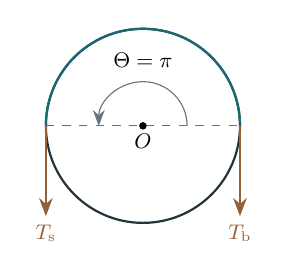
\begin{tikzpicture}[scale=0.85,transform shape]
\draw[object] (0,0) circle (1.45);
\draw[traj] (-1.45,0) arc[start angle=180,end angle=0,radius=1.45];
\draw[guide] (-1.45,0)--(1.45,0);\fill (0,0) circle (1.6pt) node[below] {$O$};
\draw[force] (-1.45,0)--(-1.45,-1.35) node[below] {$T_{\rm s}$};
\draw[force] (1.45,0)--(1.45,-1.35) node[below] {$T_{\rm b}$};
\draw[axis] (.66,0) arc[start angle=0,end angle=180,radius=.66];
\node at (0,.98) {$\Theta=\pi$};
\end{tikzpicture}
\figcaption{变图2.1V2\quad 半圈接触弧的包角为 $\pi$。}
\end{minipage}\end{center}
\item 给定 $n$ 和 $M/m$，求最小静摩擦系数。从 $\ln(M/m)\leq2\pi n\mu$ 得 $\mu_{\min}=\ln(M/m)/(2\pi n)$。变图2.1V3 固定15圈，曲线纵坐标为 $e^{30\pi\mu}$。横线100与曲线相交的位置给出 $\mu_{\min}=\ln100/(30\pi)=0.04886\cdots$。更大的 $\mu$ 使曲线上限超过100，留下静摩擦余量。
\begin{center}\begin{minipage}{.98\linewidth}\centering
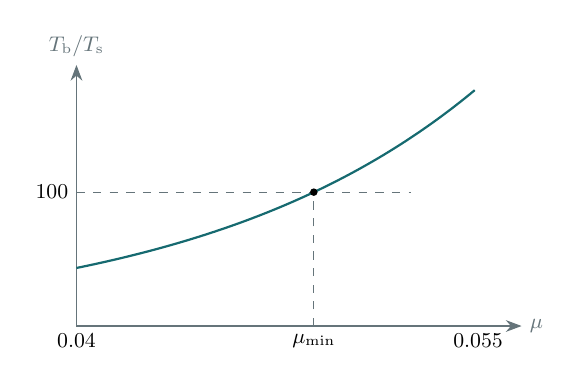
\begin{tikzpicture}[scale=0.85,transform shape]
\draw[axis] (0,0)--(6.65,0) node[right] {$\mu$};
\draw[axis] (0,0)--(0,3.9) node[above] {$T_{\rm b}/T_{\rm s}$};
\draw[traj,domain=.04:.055,samples=76] plot ({400*(\x-.04)},{.02*exp(30*pi*\x)});
\draw[guide] (0,2)--(5,2);\node[left] at (0,2) {$100$};
\draw[guide] ({400*(ln(100)/(30*pi)-.04)},0)--({400*(ln(100)/(30*pi)-.04)},2);
\fill ({400*(ln(100)/(30*pi)-.04)},2) circle (1.6pt);
\node[below] at ({400*(ln(100)/(30*pi)-.04)},0) {$\mu_{\min}$};
\node[below] at (0,0) {$0.04$};\node[below] at (6,0) {$0.055$};
\end{tikzpicture}
\figcaption{变图2.1V3\quad 15圈时，承受质量比100所需的临界摩擦系数。}
\end{minipage}\end{center}
\item 固定从端1到端2量角，将两端张力对调，平衡条件怎样写？局部有 $|\dd\ln T|\leq\mu\dd\theta$，积分给 $|\ln(T_2/T_1)|\leq\mu\Theta$。给定两端值，取 $\ln(T/T_1)=(\theta/\Theta)\ln(T_2/T_1)$ 即可达到这两个端值，且满足局部摩擦上限。变图2.1V4 分别画出正、负两种斜率。$T_2>T_1$ 时潜在滑动向端2，摩擦朝端1；对调后两方向同时反转。
\begin{center}\begin{minipage}{.98\linewidth}\centering
\begin{tikzpicture}[scale=0.85,transform shape]
\draw[axis] (0,0)--(6.65,0) node[right] {$\theta/\Theta$};
\draw[axis] (0,-2.05)--(0,2.45) node[above] {$\ln(T/T_1)$};
\draw[traj] (0,0)--(6,1.6) node[right] {$T_2>T_1$};
\draw[traj,dashed] (0,0)--(6,-1.6) node[right] {$T_2<T_1$};
\draw[guide] (6,-1.6)--(6,1.6);\node[below right] at (6,0) {$1$};
\draw[motion] (3.9,1.82)--(2.3,1.82) node[midway,above] {摩擦};
\draw[motion] (2.3,-1.84)--(3.9,-1.84) node[midway,below] {摩擦};
\end{tikzpicture}
\figcaption{变图2.1V4\quad 固定从端1到端2量角，两端张力对调时对数斜率和摩擦方向都改变。}
\end{minipage}\end{center}
\end{enumerate}

\clearpage

\pdfbookmark[2]{第 2 题 旋转斜杆上小环的稳定位置}{q2}

\section*{第 2 题\quad 旋转斜杆上小环的稳定位置}

\tagline{M-02-02}

细杆的一端支于地面，以恒定角速度 $\omega>0$ 绕过支点的竖直轴旋转。杆与水平地面的夹角为 $\alpha$，$0<\alpha<\pi/2$。质量 $m$ 的小环套在杆上，静摩擦系数为 $\mu\geq0$。求小环能相对杆保持静止、随杆转动的位置范围，位置以距支点的长度 $L\geq0$ 表示。杆长若有限，取所得范围与实际杆长的交集。

\begin{center}\begin{minipage}{\linewidth}\centering\begin{tikzpicture}

\draw[object] (-.5,0)--(5,0);\draw[axis] (0,-.2)--(0,3.6) node[above] {转轴};
\draw[object,line width=1.2pt] (0,0)--(4,3);\draw[object,fill=accent!15] (2.4,1.8) circle(.15);
\draw[guide] (0,1.8)--(2.4,1.8) node[midway,above] {$L\cos\alpha$};
\draw[thin,<->] (.27,-.36)--(2.67,1.44) node[midway,below right] {$L$};
\draw (.8,0) arc(0:36.87:.8);\node at (1.03,.32) {$\alpha$};
\node[above right] at (2.4,1.8) {$m$};\node[below] at (0,0) {$O$};
\draw[motion] (-.45,3.1) arc(150:-120:.5 and .18) node[left] {$\omega$};

\end{tikzpicture}
\figcaption{图 2.2\quad 小环相对杆静止时，对地作半径 $L\cos\alpha$ 的水平圆周运动。}
\end{minipage}\end{center}

\Needspace{5\baselineskip}

\pdfbookmark[3]{题型定位}{q2-h0}

\subsection*{题型定位}

旋转斜杆上静摩擦允许的位置范围。先由小环的圆周运动求各位置所需的摩擦与支持力，再把两侧静摩擦限值分别换成位置不等式。

\Needspace{5\baselineskip}

\pdfbookmark[3]{知识点}{q2-h1}

\subsection*{知识点}

共转时小环的水平运动半径为 $L\cos\alpha$。在地面系用重力、支持力和摩擦力产生向轴加速度；在旋转系可沿杆投影重力和离心力，再用摩擦平衡。$|f|\leq\mu N$ 给出共转位置范围，滑动后的动力学由沿杆净力决定。


\Needspace{5\baselineskip}

\pdfbookmark[3]{物理图像}{q2-h2}

\subsection*{物理图像}

解图2.2A 中，支持力沿杆法线朝左上，小环的圆周加速度水平向轴。小环越往杆的高处，维持共转所需的向心力越大。解图2.2B 的所需摩擦从沿杆向上逐步减到零，再转成沿杆向下。$L_0$ 是摩擦换向的位置。

\Needspace{5\baselineskip}

\pdfbookmark[3]{解题入口}{q2-h3}

\subsection*{解题入口}

取 $x$ 水平向外，$z$ 竖直向上，$f$ 沿杆向上为正。解水平与竖直两式得 $f,N$，写 $f=m\omega^2\cos^2\alpha(L_0-L)$。再分别处理 $f\leq\mu N$ 和 $f\geq-\mu N$。下侧系数 $c(c+\mu s)$ 恒正，上侧系数 $c(c-\mu s)$ 的符号决定是否有有限上限。

\Needspace{5\baselineskip}

\pdfbookmark[3]{标准解法}{q2-h4}

\subsection*{标准解法}

设小环距支点为 $L$，其水平圆周半径为 $r=L\cos\alpha$。小环保持 $L$ 不变时，随杆沿半径 $r$ 作水平圆周运动，地面系中的加速度为 $\omega^2r$，指向转轴。取水平向外为 $x$ 正向，竖直向上为 $z$ 正向，摩擦 $f$ 沿杆向上为正。
\begin{center}\begin{minipage}{\linewidth}\centering\begin{tikzpicture}

\draw[guide] (-1,-.75)--(1.6,1.2);\fill (0,0) circle(2pt);
\draw[force] (0,0)--(-.9,1.2) node[above left] {$N$};
\draw[force] (0,0)--(.4,.3) node[above right] {$f$};
\draw[force] (0,0)--(0,-1.5) node[below] {$mg$};
\draw[motion] (0,-.35)--(-1.4,-.35) node[below left] {$\vect a$};
\node[align=left] at (4.8,.9) {水平向左的$\vect a$指向转轴\\摩擦的正方向沿杆向上\\$f<0$对应摩擦沿杆向下};

\end{tikzpicture}
\figcaption{解图 2.2A\quad 小环的重力、支持力、摩擦与向心加速度。}
\end{minipage}\end{center}
解图 2.2A 画出重力、支持力与摩擦力。支持力垂直杆、朝斜上方，两个方向的运动方程为
\[
-N\sin\alpha+f\cos\alpha=-m\omega^2L\cos\alpha,
\qquad N\cos\alpha+f\sin\alpha=mg.
\]
将第一式乘 $\cos\alpha$、第二式乘 $\sin\alpha$ 后相加，消去 $N$；用另一组投影消去 $f$，得到
\[
f=m(g\sin\alpha-\omega^2L\cos^2\alpha),\qquad
N=m\cos\alpha(g+\omega^2L\sin\alpha)>0.
\]
\subsubsection*{摩擦方向随位置改变}
令
\[
L_0=\frac{g\sin\alpha}{\omega^2\cos^2\alpha},
\qquad f=m\omega^2\cos^2\alpha(L_0-L).
\]
$L<L_0$ 时，重力沿杆的下滑作用较强，摩擦向上；$L>L_0$ 时，维持圆周运动所需的接触合力要求摩擦向下；$L=L_0$ 时无须摩擦。图2.2A 的摩擦箭头沿杆向上，用来规定 $f$ 的正方向；若求得 $f<0$，实际摩擦沿杆向下。

\subsubsection*{分别求两端限制}
记 $s=\sin\alpha$、$c=\cos\alpha$。由 $f\leq\mu N$，整理得
\[
g(s-\mu c)\leq\omega^2Lc(c+\mu s).
\]
右边的系数严格为正，再结合 $L\geq0$，下限为
\[
\boxed{L_-=\max\left(0,\frac{g(s-\mu c)}{\omega^2c(c+\mu s)}\right)}.
\]
因此 $\mu\geq\tan\alpha$ 时，小环可以一直放到支点附近。
另一侧 $f\geq-\mu N$ 给出
\[
\omega^2Lc(c-\mu s)\leq g(s+\mu c).
\]
若 $c-\mu s>0$，可除以正系数，得到有限上限；若 $c-\mu s\leq0$，对任何 $L\geq0$ 左边都不大于零，该条件自动满足。因此
\[
\boxed{L\in\begin{cases}
[L_-,L_+],&\mu<\cot\alpha,\\
[L_-,\infty),&\mu\geq\cot\alpha,
\end{cases}\quad
L_+=\frac{g(s+\mu c)}{\omega^2c(c-\mu s)}}.
\]
若杆的实际长度为 $\ell$，还要与 $[0,\ell]$ 取交集。两个代数端点均为正且有限时，即 $\mu<\min(\tan\alpha,\cot\alpha)$，区间宽度为
\[
L_+-L_-=\frac{2\mu g}{\omega^2c^3(1-\mu^2\tan^2\alpha)}.
\]
\subsubsection*{可维持位置与动力学稳定性}
$\mu=0$ 时区间缩为 $L_0$。若环离开该点，沿杆的净驱动力为 $m\omega^2c^2(L-L_0)$，与偏离同向，故该无摩擦平衡不稳定。有静摩擦时，允许区间中的每个位置各有一个所需的 $f$。若小环在区间内的另一位置以相对杆静止的状态释放，静摩擦可在该位置维持共转。回到某一固定位置的动力学问题则要由运动后的受力决定。
\subsubsection*{受力消元、区间宽度与摩擦曲线}
为看清支持力和摩擦怎样分工，将水平运动方程乘$\cos\alpha$、
竖直方程乘$\sin\alpha$相加，得到
\[
f(\cos^2\alpha+\sin^2\alpha)
=mg\sin\alpha-m\omega^2L\cos^2\alpha.
\]
改将水平式乘$-\sin\alpha$、竖直式乘$\cos\alpha$相加，
则$N=mg\cos\alpha+m\omega^2L\sin\alpha\cos\alpha$。
竖直方向的加速度为零，所以图2.2A 中支持力与摩擦力的竖直分量之和等于重力。当 $f$ 变号时，摩擦的竖直分量也随之改变。

在两个端点均正且有限的情形，通分可把宽度展开为
\[
\begin{aligned}
L_+-L_-&=\frac g{\omega^2c}
\frac{(s+\mu c)(c+\mu s)-(s-\mu c)(c-\mu s)}
{c^2-\mu^2s^2}\\
&=\frac g{\omega^2c}
\frac{2\mu(s^2+c^2)}{c^2-\mu^2s^2}
=\frac{2\mu g}{\omega^2c^3(1-\mu^2\tan^2\alpha)}.
\end{aligned}
\]
这条宽度式适用于两端都由摩擦等式确定的有限区间。若下限取 $0$，宽度改为 $L_+$；若上限不限，则还要按实际杆长决定可用区间。

解图2.2B取$\alpha=45^\circ,\mu=0.20$作例子。
实线是维持共转所需的$f$，两虚线是材料可提供的$\pm\mu N$。
在实线位于两虚线之间的区段，静摩擦能维持小环共转。
\begin{center}\begin{minipage}{\linewidth}\centering
\begin{tikzpicture}[x=1.6cm,y=2cm]
\fill[accent!8] (.94281,-.78) rectangle (2.12132,.83);
\draw[axis] (-.12,0)--(3.05,0) node[right] {$\lambda=\omega^2L/g$};
\draw[axis] (0,-.82)--(0,.92) node[above] {$f/(mg)$};
\draw[guide,domain=0:2.8] plot(\x,{.141421+.1*\x});
\draw[guide,domain=0:2.8] plot(\x,{-.141421-.1*\x});
\draw[thin,domain=0:2.8] plot(\x,{.707107-.5*\x});
\draw[traj,line width=1.3pt,domain=.94281:2.12132] plot(\x,{.707107-.5*\x});
\draw[guide] (.94281,0)--(.94281,.2357);
\draw[guide] (2.12132,0)--(2.12132,-.35355);
\fill (.94281,.2357) circle(1pt); \fill (2.12132,-.35355) circle(1pt);
\node[below] at (.94281,0) {$L_-$};
\node[above] at (1.41421,0) {$L_0$};
\node[above] at (2.12132,0) {$L_+$};
\node[right] at (2.8,.42142) {$+\mu N/(mg)$};
\node[right] at (2.8,-.42142) {$-\mu N/(mg)$};
\node[above right] at (.1,.6571) {所需摩擦};
\end{tikzpicture}
\figcaption{解图2.2B\quad 接触力可实现的区间；三个标记表示相应$L$在无量纲横轴上的位置。}
\end{minipage}\end{center}
$L$减小到$L_-$以下，所需向上摩擦超出上界，小环出现下滑趋势；
$L$增大到有限的$L_+$以上，所需向下摩擦超出下界，小环出现上滑趋势。
在$L_0$处支持力独自平衡竖直重力并提供向心力，摩擦恰为零。
图2.2B 的交点给出允许共转的端点。区间内实线到两条虚线都有余量，各处可分别以所需的静摩擦保持位置。


\Needspace{5\baselineskip}

\pdfbookmark[3]{关键洞察}{q2-h5}

\subsection*{关键洞察}

位置 $L$ 同时决定所需摩擦和法向支持力。图2.2B 的实线和两虚线分别画这两类量。实线在两虚线之间时，材料可提供所需的摩擦。改变 $\mu$ 会改变虚线斜率，可能使其中一侧永远保持余量。

\Needspace{5\baselineskip}

\pdfbookmark[3]{易错点}{q2-h6}

\subsection*{易错点}

\begin{itemize}
\item 把 $|f|=\mu N$ 用于两端，区间内部按实际共转所需的 $f$ 取值。
\item 水平向心半径为 $L\cos\alpha$，沿杆的向心加速度投影大小为 $\omega^2L\cos^2\alpha$。
\item $f>0$ 表示沿杆向上，$f<0$ 表示沿杆向下。$L_0$ 将两种方向分开。
\item 写上限前看 $c-\mu s$。它非正时，上侧不等式对所有 $L\geq0$ 成立。
\end{itemize}

\Needspace{5\baselineskip}

\pdfbookmark[3]{课堂讲解建议}{q2-h7}

\subsection*{课堂讲解建议}

先在解图2.2A 中请学生画出水平向心加速度，并指出竖直加速度为零。问“哪一点无需摩擦”，令 $f(L)=0$ 得 $L_0$，再解释此处支持力独自提供竖直平衡和向心力。用解图2.2B 画出所需摩擦与 $\pm\mu N$，问上侧分母为零时发生什么。变图2.2V3 中，所需摩擦与下限曲线平行且始终在其上方，故这一条件不限制最大位置。最后在无摩擦情形给小环一个沿杆扰动，由净驱动力与位移同向判断不稳定。

\Needspace{5\baselineskip}

\pdfbookmark[3]{变式训练}{q2-h8}

\subsection*{变式训练}

\begin{enumerate}
\item 无摩擦时，求共转位置并判断稳定性。$f=0$ 给出唯一的 $L_0=g\sin\alpha/(\omega^2\cos^2\alpha)$。小环发生沿杆运动时，角速度仍由杆限定。将惯性系加速度沿杆投影，得
\[
m\ddot L=m\omega^2 L\cos^2\alpha-mg\sin\alpha=m\omega^2\cos^2\alpha(L-L_0).
\]
变图2.2V1 的直线斜率为正，$L>L_0$ 时净力向上，$L<L_0$ 时净力向下。若从偏差 $\delta L_i$ 处静止释放，$\delta L(t)=\delta L_i\cosh(\omega\cos\alpha\,t)$，偏差的绝对值增长，故该平衡位置不稳定。
\begin{center}\begin{minipage}{.98\linewidth}\centering
\begin{tikzpicture}[scale=0.85,transform shape]
\draw[axis] (0,0)--(6.65,0) node[right] {$L/L_0$};
\draw[axis] (0,-2.35)--(0,2.5) node[above] {$F_\parallel/(mg\sin\alpha)$};
\draw[traj] (0,-2)--(6,2);\fill (3,0) circle (1.6pt) node[above left] {$L=L_0$};\node[below] at (3,0) {$1$};
\draw[guide] (4.5,0)--(4.5,1);\draw[guide] (1.5,0)--(1.5,-1);
\draw[force] (4.5,0)--(4.5,1);\draw[force] (1.5,0)--(1.5,-1);
\node[above right] at (4.5,1) {$\delta L>0$};\node[below right] at (1.5,-1) {$\delta L<0$};
\end{tikzpicture}
\figcaption{变图2.2V1\quad 无摩擦时，沿杆净力的方向与位移偏差相同。}
\end{minipage}\end{center}
\item 固定 $\alpha,\mu$，将角速度增至两倍，有限允许区间怎样变？端点式中的角速度只出现在 $\omega^2$ 分母中，零下限保持为零，两个非零端点均缩至四分之一，有限区间的宽度也缩至四分之一。变图2.2V2 取 $\alpha=45^\circ,\mu=0.20$，用角速度加倍前的 $L_{0,\omega}$ 归一化，最初的区间为 $[2/3,3/2]$，角速度加倍后为 $[1/6,3/8]$。若杆长有限，再分别与实际杆段取交集。
\begin{center}\begin{minipage}{.98\linewidth}\centering
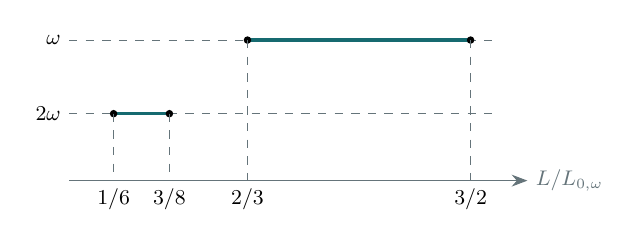
\begin{tikzpicture}[scale=0.85,transform shape]
\draw[axis] (0,0)--(6.85,0) node[right] {$L/L_{0,\omega}$};
\draw[guide] (0,1)--(6.35,1);\draw[guide] (0,2.1)--(6.35,2.1);
\draw[traj,very thick] ({4*2/3},2.1)--(6,2.1);\draw[traj,very thick] ({4/6},1)--(1.5,1);
\foreach \x/\y in {2.66667/2.1,6/2.1,.66667/1,1.5/1}{\fill (\x,\y) circle (1.6pt);\draw[guide] (\x,\y)--(\x,0);}
\node[left] at (0,2.1) {$\omega$};\node[left] at (0,1) {$2\omega$};
\node[below] at (.66667,0) {$1/6$};\node[below] at (1.5,0) {$3/8$};
\node[below] at (2.66667,0) {$2/3$};\node[below] at (6,0) {$3/2$};
\end{tikzpicture}
\figcaption{变图2.2V2\quad 用角速度加倍前的 $L_{0,\omega}$ 作长度单位，实线段为两种角速度的允许区间。}
\end{minipage}\end{center}
\item 当 $\cos\alpha-\mu\sin\alpha\leq0$ 时，确定上侧条件。将 $f\geq-\mu N$ 写成
\[
f+\mu N=mg(s+\mu c)+m\omega^2Lc(\mu s-c)\geq0.
\]
此时右式的常数项为正，斜率非负，因此对所有 $L\geq0$ 成立。变图2.2V3 取 $\alpha=60^\circ,\mu=\cot\alpha$，实线与下侧虚线平行，实际起点由上侧虚线交点给出 $L_-=L_0/3$。杆无限长时允许区间为 $[L_-,\infty)$，实际杆长为 $\ell$ 时取它与 $[0,\ell]$ 的交集。
\begin{center}\begin{minipage}{.98\linewidth}\centering
\begin{tikzpicture}[scale=0.85,transform shape]
\draw[axis] (0,0)--(6.7,0) node[right] {$x=L/L_0$};
\draw[axis] (0,-2.75)--(0,2.82) node[above] {$f/(mg\sin\alpha)$};
\draw[traj] (0,1)--(6,-1) node[right] {$f$};
\draw[traj,dashed] (0,{1/3})--(6,{7/3}) node[right] {$+\mu N$};
\draw[traj,dashed] (0,{-1/3})--(6,{-7/3}) node[right] {$-\mu N$};
\fill (1,{2/3}) circle (1.6pt) node[above left] {$L_-$};\draw[guide] (1,0)--(1,{2/3});
\node[below] at (1,0) {$1/3$};\node[below] at (3,0) {$1$};
\end{tikzpicture}
\figcaption{变图2.2V3\quad 取 $\alpha=60^\circ,\mu=\cot\alpha$，实线始终高于下侧虚线。各力以 $mg\sin\alpha$ 归一。}
\end{minipage}\end{center}
\item 取 $\alpha=45^\circ,\mu=0.20$，求允许位置并比较两端到 $L_0$ 的距离。$L_0=\sqrt2g/\omega^2$。设 $x=L/L_0$，则 $f/(mg\sin\alpha)=1-x$，两条摩擦限值为 $\pm0.20(1+x)$。变图2.2V4 中，由 $1-x=0.20(1+x)$ 和 $1-x=-0.20(1+x)$ 分别读出 $x_-=2/3,x_+=3/2$，所以
\[
L_- = \frac{2\sqrt2g}{3\omega^2},\qquad L_+ = \frac{3\sqrt2g}{2\omega^2}.
\]
两端到 $L_0$ 的距离分别为 $L_0/3$ 与 $L_0/2$。支持力随 $L$ 增大，图中两条限值之间的宽度也增大，允许区间向高处伸得更远。
\begin{center}\begin{minipage}{.98\linewidth}\centering
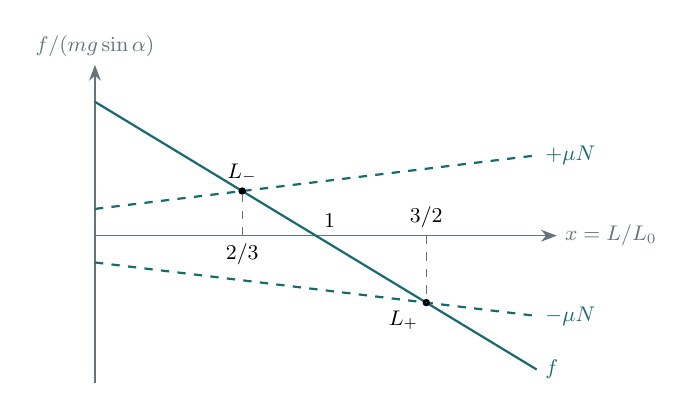
\begin{tikzpicture}[scale=0.85,transform shape]
\draw[axis] (0,0)--(6.9,0) node[right] {$x=L/L_0$};
\draw[axis] (0,-2.2)--(0,2.55) node[above] {$f/(mg\sin\alpha)$};
\draw[traj] (0,2)--(6.6,-2) node[right] {$f$};
\draw[traj,dashed] (0,.4)--(6.6,1.2) node[right] {$+\mu N$};
\draw[traj,dashed] (0,-.4)--(6.6,-1.2) node[right] {$-\mu N$};
\fill (2.2,{2/3}) circle (1.6pt) node[above] {$L_-$};\fill (4.95,-1) circle (1.6pt) node[below left] {$L_+$};
\draw[guide] (2.2,0)--(2.2,{2/3});\draw[guide] (4.95,0)--(4.95,-1);
\node[below] at (2.2,0) {$2/3$};\node[above right] at (3.3,0) {$1$};\node[above] at (4.95,0) {$3/2$};
\end{tikzpicture}
\figcaption{变图2.2V4\quad $\alpha=45^\circ,\mu=0.20$ 时，两个端点分别由两条虚线与实线的交点确定。}
\end{minipage}\end{center}
\end{enumerate}

\clearpage

\pdfbookmark[2]{第 3 题 球壳内壁水平圆周运动的速度范围}{q3}

\section*{第 3 题\quad 球壳内壁水平圆周运动的速度范围}

\tagline{M-02-03}

半径 $R$ 的空心球壳绕竖直直径匀速转动，内壁上一可视为质点的小球相对球壳静止，随球壳沿水平纬度圈以速率 $v$ 运动。小球位于下半球，球心至小球的连线与竖直向下方向的夹角为 $\theta$，$0<\theta<\pi/2$。静摩擦系数为 $\mu\geq0$。求在该纬度能维持共转的速率范围。
\par\smallskip\begin{center}\begin{minipage}{\linewidth}\centering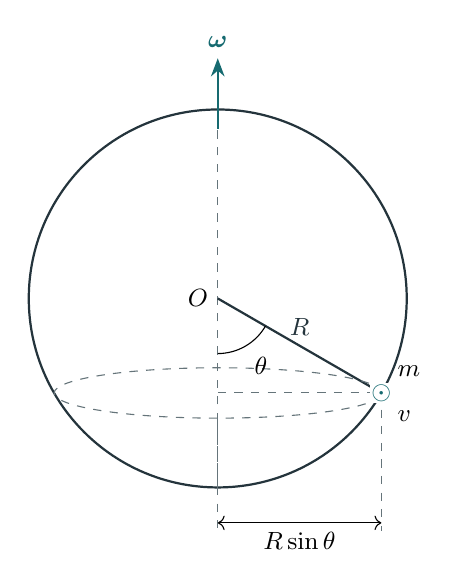
\begin{tikzpicture}
\draw[object] (0,0) circle(2.4);
\draw[guide] (0,-2.4)--(0,2.35);
\coordinate (B) at (2.078,-1.2);
\draw[object] (0,0)--(B) node[midway,above] {$R$};
\draw[guide] (0,-1.2) ellipse(2.078 and .32);
\draw[guide] (0,-1.2)--(B);
\draw[guide] (0,-1.55)--(0,-2.95);
\draw[guide] (B)--(2.078,-2.95);
\draw[<->] (0,-2.85)--(2.078,-2.85) node[midway,below] {$R\sin\theta$};
\node[fill=white,inner sep=.4pt,text=accent] at (B) {$\odot$};
\node[above right] at (2.16,-1.12) {$m$};
\node[below right] at (2.16,-1.3) {$v$};
\node[left] at (0,0) {$O$};
\draw (0,-.7) arc(-90:-30:.7);
\node at (.55,-.85) {$\theta$};
\draw[motion] (0,2.15)--(0,3.05) node[above] {$\boldsymbol\omega$};
\end{tikzpicture}
\figcaption{图 2.3\quad 纬度圈半径为$R\sin\theta$；$\odot$表示周向速度垂直子午面朝向观察者。}
\end{minipage}\end{center}

\Needspace{5\baselineskip}

\pdfbookmark[3]{题型定位}{q3-h0}

\subsection*{题型定位}

球壳固定纬圈上的共转问题。给定纬度改变速率，静摩擦的方向随向心加速度改变。把两侧摩擦上限分别转成速率条件，可与第2题给定速率求位置范围的做法对照。

\Needspace{5\baselineskip}

\pdfbookmark[3]{知识点}{q3-h1}

\subsection*{知识点}

水平圆周运动的加速度朝向转轴。支持力沿球面法线，静摩擦沿经线，两者的水平和竖直分量共同满足牛顿第二定律。把 $|f|\leq\mu N$ 拆成两侧不等式，再与 $v^2\geq0$ 合用，就能区分低速和高速的可行范围。


\Needspace{5\baselineskip}

\pdfbookmark[3]{物理图像}{q3-h2}

\subsection*{物理图像}

图2.3 的 $\odot$ 表示周向速度垂直子午面朝向观察者。图上的 $R$ 是球面半径，$R\sin\theta$ 是小球到转轴的距离。解图2.3A 中重力向下、支持力向球心，水平合力向转轴。慢于无摩擦速率时，摩擦沿经线向上，快于该速率时，摩擦沿经线向下。若所需摩擦达到 $\mu N$，便到达该侧的速率端点。

\Needspace{5\baselineskip}

\pdfbookmark[3]{解题入口}{q3-h3}

\subsection*{解题入口}

以 $r=R\sin\theta$ 表示纬圈半径，按解图2.3A 规定向上的经线摩擦为正。水平方向取向轴、竖直取向上，列式
\[
\begin{cases}
N\sin\theta-f\cos\theta=\dfrac{mv^2}{r},\\
N\cos\theta+f\sin\theta=mg,\\
r=R\sin\theta.
\end{cases}
\]
按两轴分别求出 $N,f$，再把 $f\leq\mu N$ 和 $f\geq-\mu N$ 化为 $a=v^2/r$ 的条件。低速侧结合 $a\geq0$，高速侧根据 $\cos\theta-\mu\sin\theta$ 的符号判断是否存在有限上限，最后由 $v=\sqrt{ar}$ 还原速率。

\Needspace{5\baselineskip}

\pdfbookmark[3]{标准解法}{q3-h4}

\subsection*{标准解法}

匀速共转时，小球沿纬圈的切向加速度为零。重力与支持力都在子午面内，故摩擦的周向分量为零，只有沿经线的分量。取过球心和小球的竖直截面，$\theta$ 从竖直向下的半径量起；图2.3 中，从小球到转轴的水平距离是纬圈半径 $\rho=R\sin\theta$。规定切线沿经线上行为摩擦力的正方向。
\begin{center}\begin{minipage}{\linewidth}\centering\begin{tikzpicture}

\fill (0,0) circle(2pt);\draw[guide] (-.75,-1.3)--(.9,1.56);
\draw[force] (0,0)--(-1.3,.75) node[above left] {$N$};
\draw[force] (0,0)--(.43301,.75) node[above right] {$f>0$};
\draw[force] (0,0)--(0,-1.5) node[below] {$mg$};
\draw[motion] (0,-.35)--(-1.4,-.35) node[below left] {$v^2/\rho$};
\draw[axis] (3.6,-.5)--(2.6,-.5) node[midway,below] {向轴为正};
\node[align=left] at (5.7,1.1) {$N\sin\theta-f\cos\theta=mv^2/\rho$\\$N\cos\theta+f\sin\theta=mg$};

\end{tikzpicture}
\figcaption{解图 2.3A\quad 共转小球的重力、支持力、摩擦及向轴加速度。}
\end{minipage}\end{center}
解图 2.3A 中，支持力 $N$ 沿球面法线指向球心；$f>0$ 朝斜上方。小球的加速度水平指向转轴，竖直加速度为零，所以
\[
N\sin\theta-f\cos\theta=\frac{mv^2}{\rho},
\qquad N\cos\theta+f\sin\theta=mg.
\]
记 $a=v^2/\rho$。两式分别作切向与法向的线性组合，得到
\[
f=m(g\sin\theta-a\cos\theta),\qquad
N=m(g\cos\theta+a\sin\theta)>0.
\]
这样先得到任一速率下维持共转所需的 $f$ 和 $N$。材料允许的范围是 $-\mu N\leq f\leq\mu N$，其中等号给出摩擦达到极限的端点。

\subsubsection*{无摩擦速度与两个临界趋势}
令 $f=0$，得 $a=g\tan\theta$，即
\[
\boxed{v_0=\sin\theta\sqrt{\frac{gR}{\cos\theta}}}.
\]
当 $v<v_0$ 时需要向上的摩擦，阻止下滑；当 $v>v_0$ 时需要向下的摩擦，阻止上滑。记 $s=\sin\theta$、$c=\cos\theta$，由 $f\leq\mu N$ 得
\[
g(s-\mu c)\leq a(c+\mu s).
\]
因为 $c+\mu s>0$，再用 $a\geq0$，得到
\[
a\geq g\max\left(0,\frac{s-\mu c}{c+\mu s}\right).
\]
乘以 $\rho=Rs$，速率下限为
\[
\boxed{v_{\min}=\sqrt{gRs\max\left(0,\frac{s-\mu c}{c+\mu s}\right)}}.
\]
下限为零对应 $\mu\geq\tan\theta$。在 $v=0$ 时，沿经线向上的摩擦大小为 $mg\sin\theta$，法向力为 $mg\cos\theta$，这个条件恰好允许两者与重力平衡。

另一侧 $f\geq-\mu N$ 整理为
\[
a(c-\mu s)\leq g(s+\mu c).
\]
当 $c-\mu s>0$ 时有有限上限，反之没有有限上限。因此
\[
\boxed{v_{\max}=\begin{cases}
\sqrt{gRs(s+\mu c)/(c-\mu s)},&\mu<\cot\theta,\\
\infty,&\mu\geq\cot\theta,
\end{cases}\qquad v_{\min}\leq v\leq v_{\max}}.
\]
高速时 $f<0$，其绝对值与 $N$ 的比趋于 $\cot\theta$。当 $\mu\geq\cot\theta$，任何有限高速所需的向下摩擦都在材料范围内。

\subsubsection*{无摩擦与接触条件}
$\mu=0$ 时两端重合于 $v_0$。在题定的下半球，$g\cos\theta>0$，而 $a\sin\theta\geq0$，两项相加使 $N$ 始终为正。这里求的是随壳共转所需的静摩擦。若球壳固定而小球沿壁滑动，摩擦沿相对速度的反向，应按滑动时的切向运动列式。
\subsubsection*{两个临界端点的受力代入}
低速端由上行摩擦达到极限确定时，解图2.3A中的切向方程给出
\[
g\sin\theta-a_{\min}\cos\theta
=\mu(g\cos\theta+a_{\min}\sin\theta).
\]
若存在有限的高速端，该端的下行摩擦达到极限，得到
\[
g\sin\theta-a_{\max}\cos\theta
=-\mu(g\cos\theta+a_{\max}\sin\theta).
\]
两式的正负号对应图中同一条经线的相反方向。
第一式移项后，$a$ 的系数总为正。当解出的代数下限为负时，所有非负 $a$ 都满足这一侧条件，速率从零起算。第二式移项后，若 $c-\mu s\leq0$，左侧对一切 $a\geq0$ 都小于或等于零，而右侧为正，于是这一侧给出的范围延伸到任意大速率。


\Needspace{5\baselineskip}

\pdfbookmark[3]{关键洞察}{q3-h5}

\subsection*{关键洞察}

给定纬度时，$N$ 随速率增大而增加，$f$ 则由正变负。低速侧的极限由向上摩擦决定，高速侧由向下摩擦决定，两个端点以各自当时的 $\mu N$ 为准。静止时的需求比为 $\tan\theta$，高速极限为 $\cot\theta$。

\Needspace{5\baselineskip}

\pdfbookmark[3]{易错点}{q3-h6}

\subsection*{易错点}

\begin{itemize}
\item 水平向心加速度的分母取纬圈半径 $R\sin\theta$。
\item 以同一经线上行方向记 $f$ 的符号，高速分支的 $f$ 为负。
\item 上下限处的支持力随速率变化。两侧分别使用当时的 $N$。
\item 当 $\cos\theta-\mu\sin\theta\leq0$，高速侧不等式对所有非负 $a$ 成立。
\end{itemize}

\Needspace{5\baselineskip}

\pdfbookmark[3]{课堂讲解建议}{q3-h7}

\subsection*{课堂讲解建议}

先遮住解图2.3A 的摩擦箭头，问“小球用哪个速度时可以省掉这支箭头？”由 $N\cos\theta=mg$ 得
\[
v_0=\sin\theta\sqrt{\frac{gR}{\cos\theta}}.
\]
随后问“速度增大时，支持力和摩擦怎样变？”让学生从 $N=m(g\cos\theta+a\sin\theta)$ 读出支持力增大，再从 $f$ 的符号画出向下摩擦。最后对着变图2.3V4 比较两个摩擦阈值。取 $\theta=30^\circ$ 和 $60^\circ$，请学生分别说明同一种材料可以允许静止还是允许任意高速度。

\Needspace{5\baselineskip}

\pdfbookmark[3]{变式训练}{q3-h8}

\subsection*{变式训练}

\begin{enumerate}
\item 取 $\mu=0$，求能维持共转的速率。摩擦力为零，解图2.3A 的竖直平衡给 $N=mg/\cos\theta$。代入向心水平式 $mv^2/(R\sin\theta)=N\sin\theta$，得到
\[
v_0=\sin\theta\sqrt{\frac{gR}{\cos\theta}}.
\]
变图2.3V1 的支持力竖直分量恰好平衡重力，余下水平分量决定唯一的 $a_0=g\tan\theta$。两端速率都退化到 $v_0$。
\begin{center}\begin{minipage}{.98\linewidth}\centering
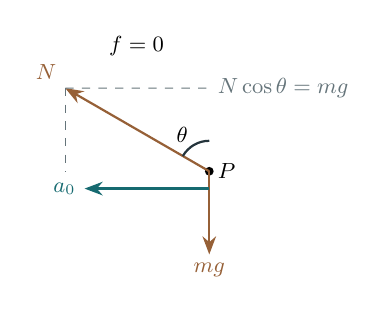
\begin{tikzpicture}[scale=.88,transform shape]
\coordinate (P) at (0,0);
\coordinate (A) at (-2.0785,1.2);
\coordinate (H) at (-2.0785,0);
\fill (P) circle(1.8pt) node[right] {$P$};
\draw[force] (P)--(A) node[above left] {$N$};
\draw[force] (P)--(0,-1.2) node[below] {$mg$};
\draw[guide] (A)--(H);
\draw[guide] (A)--(0,1.2) node[right] {$N\cos\theta=mg$};
\draw[motion] (0,-.25)--(-1.8,-.25) node[left] {$a_0$};
\draw[object] (0,.44) arc (90:150:.44);
\node at (-.39,.52) {$\theta$};
\node[above] at (-1.05,1.55) {$f=0$};
\end{tikzpicture}
\figcaption{变图2.3V1\quad 取 $\theta=60^\circ$，支持力的水平分量提供向心加速度。}
\end{minipage}\end{center}
\item 取 $\theta=45^\circ$，求速率范围。用 $q=v^2/(gR\sin\theta)$，所需摩擦比化成 $(1-q)/(1+q)$。因为 $q\geq0$，分母恒正。将 $-\mu\leq(1-q)/(1+q)\leq\mu$ 逐侧移项，得
\[
v_{\min}^2=\frac{gR}{\sqrt2}\max\left(0,\frac{1-\mu}{1+\mu}\right),\qquad
v_{\max}^2=\frac{gR}{\sqrt2}\frac{1+\mu}{1-\mu}\quad (\mu<1).
\]
当 $\mu\geq1$，范围是 $0\leq v<\infty$。变图2.3V2 取 $\mu=1/2$，阴影带内的曲线从 $q=1/3$ 到 $q=3$。曲线在 $q=1$ 处过零，摩擦方向随之反转。
\begin{center}\begin{minipage}{.98\linewidth}\centering
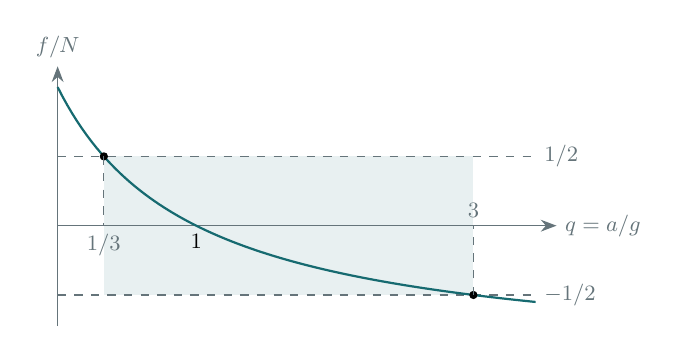
\begin{tikzpicture}[scale=.88,transform shape]
\fill[accent!10] (.667,-1) rectangle (6,1);
\draw[axis] (0,0)--(7.2,0) node[right] {$q=a/g$};
\draw[axis] (0,-1.45)--(0,2.3) node[above] {$f/N$};
\draw[guide] (0,1)--(6.9,1) node[right] {$1/2$};
\draw[guide] (0,-1)--(6.9,-1) node[right] {$-1/2$};
\draw[traj,domain=0:3.45,samples=100] plot({2*\x},{2*(1-\x)/(1+\x)});
\fill (.667,1) circle(1.7pt);\fill (6,-1) circle(1.7pt);
\draw[guide] (.667,1)--(.667,0) node[below] {$1/3$};
\draw[guide] (6,-1)--(6,0) node[above] {$3$};
\node[below] at (2,0) {$1$};
\end{tikzpicture}
\figcaption{变图2.3V2\quad 在 $45^\circ$ 纬圈取 $\mu=1/2$，两个交点给速度区间的端点。}
\end{minipage}\end{center}
\item 已知速率，求所需的最小静摩擦系数。将受力方程投到经线切向与法向，分别得到 $f=m(g\sin\theta-a\cos\theta)$ 和 $N=m(g\cos\theta+a\sin\theta)$，其中 $a=v^2/(R\sin\theta)$。最小系数在 $|f|=\mu_{\min}N$ 时取得，
\[
\mu_{\min}=\frac{|g\sin\theta-[v^2/(R\sin\theta)]\cos\theta|}{g\cos\theta+v^2/R}.
\]
变图2.3V3 取 $\theta=60^\circ$，实线给有符号比。$q=a/g$ 小于 $\sqrt3$ 时摩擦朝上，大于 $\sqrt3$ 时摩擦朝下，后半段取绝对值后反射到横轴上方。
\begin{center}\begin{minipage}{.98\linewidth}\centering
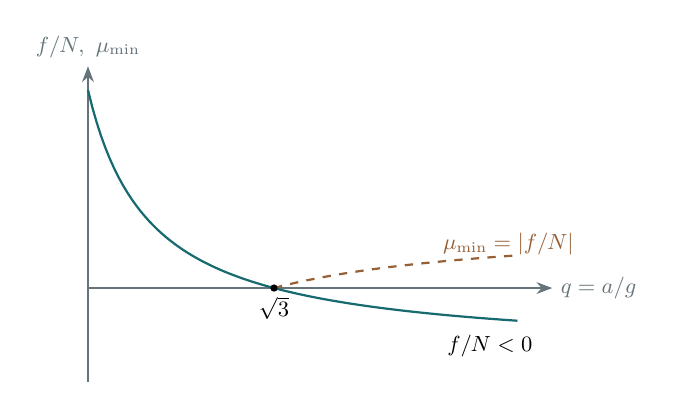
\begin{tikzpicture}[scale=.88,transform shape]
\draw[axis] (0,0)--(6.7,0) node[right] {$q=a/g$};
\draw[axis] (0,-1.35)--(0,3.2) node[above] {$f/N,\ \mu_{\min}$};
\draw[traj,domain=0:4,samples=100] plot({1.55*\x},{1.65*(.8660254-.5*\x)/(.5+.8660254*\x)});
\draw[guide,thick,color=warm,domain=1.73205:4,samples=70] plot({1.55*\x},{-1.65*(.8660254-.5*\x)/(.5+.8660254*\x)});
\fill (2.68468,0) circle(1.5pt) node[below] {$\sqrt3$};
\node[text=warm,right] at (5.0,.63) {$\mu_{\min}=|f/N|$};
\node[below] at (5.8,-.55) {$f/N<0$};
\end{tikzpicture}
\figcaption{变图2.3V3\quad 虚线为负的有符号比关于横轴的反射。}
\end{minipage}\end{center}
\item 给定材料系数，何时允许零速率，何时有任意大的速率？在 $a=0$ 时，$f/N=\tan\theta$，所以零速率要求 $\mu\geq\tan\theta$。高速时 $-f/N$ 单调增至 $\cot\theta$，任意大速率要求 $\mu\geq\cot\theta$。变图2.3V4 取 $\mu=1$。在 $30^\circ$ 纬圈，材料线高于 $\tan\theta$ 而低于 $\cot\theta$，因此允许静止但有最高速度。在 $60^\circ$ 纬圈，材料线在两阈值间的位置对调，因此有最低速率而无有限上限。$45^\circ$ 时两条阈值曲线相交，两个条件相同。
\begin{center}\begin{minipage}{.98\linewidth}\centering
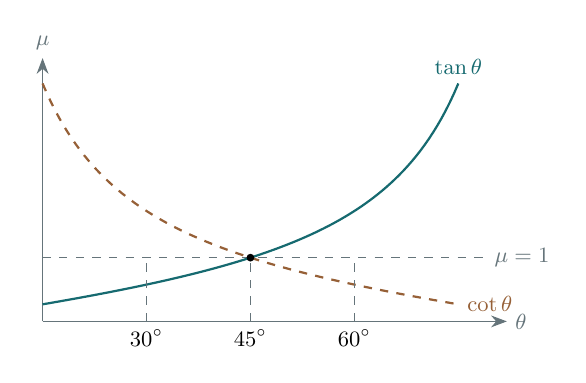
\begin{tikzpicture}[scale=.88,transform shape]
\draw[axis] (0,0)--(6.7,0) node[right] {$\theta$};
\draw[axis] (0,0)--(0,3.8) node[above] {$\mu$};
\draw[traj,domain=15:75,samples=100] plot({(\x-15)/10},{.92*tan(\x)}) node[above] {$\tan\theta$};
\draw[guide,thick,color=warm,domain=15:75,samples=100] plot({(\x-15)/10},{.92/tan(\x)}) node[right] {$\cot\theta$};
\draw[guide] (0,.92)--(6.4,.92) node[right] {$\mu=1$};
\foreach \x/\d in {1.5/30,3/45,4.5/60}{\draw[guide] (\x,0)--(\x,.92);\node[below] at (\x,0) {$\d^\circ$};}
\fill (3,.92) circle(1.6pt);
\end{tikzpicture}
\figcaption{变图2.3V4\quad 横线与两条阈值曲线比较，给出不同纬圈的静止和高速条件。}
\end{minipage}\end{center}
\end{enumerate}

\clearpage

\pdfbookmark[2]{第 4 题 光滑斜面体与滑块的约束加速度}{q4}

\section*{第 4 题\quad 光滑斜面体与滑块的约束加速度}

\tagline{M-02-04}

倾角为 $\theta$、质量为 $M$ 的斜面体放在光滑水平地面上，质量为 $m$ 的木块放在斜面上，接触面也光滑。斜面从左下向右上倾斜，$0<\theta<\pi/2$。求斜面体与木块相对地面的加速度，以及木块所受支持力。

\begin{center}\begin{minipage}{\linewidth}\centering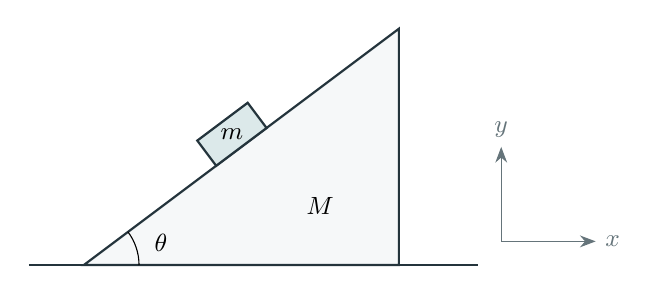
\begin{tikzpicture}

\draw[object] (-.7,0)--(5,0);\draw[object,fill=rulegray!20] (0,0)--(4,3)--(4,0)--cycle;
\begin{scope}[shift={(1.88,1.66)},rotate=36.87]\draw[object,fill=accent!15] (-.4,-.2) rectangle (.4,.2);\node at (0,0) {$m$};\end{scope}
\node at (3,.75) {$M$};\draw (.7,0) arc(0:36.87:.7);\node at (.98,.28) {$\theta$};
\draw[axis] (5.3,.3)--(6.5,.3) node[right] {$x$};\draw[axis] (5.3,.3)--(5.3,1.5) node[above] {$y$};

\end{tikzpicture}
\figcaption{图 2.4\quad 木块下滑时，斜面体向右运动；两者加速度均按地面坐标描述。}
\end{minipage}\end{center}

\Needspace{5\baselineskip}

\pdfbookmark[3]{题型定位}{q4-h0}

\subsection*{题型定位}

光滑可动斜面上的约束运动。分开两物体列动力学方程，再把木块相对斜面沿坡运动写成第四个方程。整体水平运动给出两个水平加速度的关系。

\Needspace{5\baselineskip}

\pdfbookmark[3]{知识点}{q4-h1}

\subsection*{知识点}

地面系、牛顿第二定律、接触法向、相对加速度和水平动量守恒。滑块对地加速度由斜面体的水平平动和沿坡的相对加速度合成。也可用平动斜面系中的惯性力得到同一结果。


\Needspace{5\baselineskip}

\pdfbookmark[3]{物理图像}{q4-h2}

\subsection*{物理图像}

图2.4 中，木块沿坡向左下滑，反作用力将斜面体推向右。解图2.4A 的两个支持力方向相反，水平分量分别改变两个物体的水平速度。解图2.4B 中 $OP$ 水平向右，$PQ$ 沿坡向下，两箭头首尾相接得到滑块对地的 $OQ$。

\Needspace{5\baselineskip}

\pdfbookmark[3]{解题入口}{q4-h3}

\subsection*{解题入口}

先取地面为惯性系，把木块加速度写成 $\vec a_m=a_x\hat i+a_y\hat j$，把斜面体加速度写成 $\vec a_M=a_M\hat i$。根据图2.4A，
\[
-N\sin\theta=ma_x,\qquad N\cos\theta-mg=ma_y,\qquad N\sin\theta=Ma_M.
\]
给四个未知量补上相对加速度的法向投影为零，即 $(a_x-a_M)\sin\theta-a_y\cos\theta=0$。也可在斜面体参考系加入水平向左的惯性力，再沿坡和法向分别投影。

\Needspace{5\baselineskip}

\pdfbookmark[3]{标准解法}{q4-h4}

\subsection*{标准解法}

取地面为惯性系，$x$ 向右、$y$ 向上。设斜面体加速度为 $a_M$，木块加速度分量为 $a_x,a_y$。解图2.4A 分别画出木块和斜面体的受力。木块受重力和斜面的法向支持力，斜面体受反向接触力、重力和地面支持力。
\begin{center}\begin{minipage}{\linewidth}\centering\begin{tikzpicture}

\fill (0,1) circle(2pt);\node[above right] at (0,1) {$m$};
\draw[force] (0,1)--(-.6,1.8) node[above left] {$N$};\draw[force] (0,1)--(0,-.7) node[below] {$mg$};
\draw[guide] (-.8,.4)--(1.2,1.9);
\draw[object] (4.3,.5) rectangle (5.7,1.5);\node at (5,1) {$M$};
\draw[force] (5,1.5)--(5.6,.7) node[right] {$-\vect N$};
\draw[force] (4.65,.5)--(4.65,-1.2) node[below] {$Mg$};
\draw[force] (5.35,.5)--(5.35,3) node[above] {$N_g$};
\draw[motion] (5,1)--(6.6,1) node[above] {$a_M$};

\end{tikzpicture}
\figcaption{解图 2.4A\quad 木块与斜面体分别受力；光滑地面对斜面体没有水平力。}
\end{minipage}\end{center}
因此三个运动方程为
\[
ma_x=-N\sin\theta,\qquad ma_y=N\cos\theta-mg,
\qquad Ma_M=N\sin\theta. \tag{1}
\]
这三式含有 $a_x,a_y,a_M,N$ 四个未知量。接触面光滑给出力的法向方向，木块贴在坡面上又给出一条相对运动关系。

\subsubsection*{由相对运动写接触约束}
解图 2.4B 中，加速度矢量满足 $\vect a_m=\vect a_M+\vect a_{m/M}$。规定木块沿坡向下的相对加速度大小为 $b$，则
\[
\vect a_{m/M}=(-b\cos\theta,-b\sin\theta),
\quad a_x=a_M-b\cos\theta,\quad a_y=-b\sin\theta.
\]
\begin{center}\begin{minipage}{\linewidth}\centering\begin{tikzpicture}

\coordinate (O) at (0,1.8);\coordinate (P) at (1.7,1.8);\coordinate (Q) at (-.7,0);
\draw[motion] (O)--(P) node[midway,above] {$\vect a_M$};
\draw[force] (P)--(Q) node[midway,below right] {$\vect a_{m/M}$};
\draw[motion] (O)--(Q) node[midway,left] {$\vect a_m$};
\draw[guide] (-1.1,-.3)--(2.1,2.1);\fill (O) circle(1.5pt) node[above left]{$O$};\fill (P) circle(1.5pt) node[above right]{$P$};\fill (Q) circle(1.5pt) node[below left]{$Q$};
\node[align=left] at (5.4,1.8) {$\vect a_m=\vect a_M+\vect a_{m/M}$\\相对加速度沿坡向下\\两箭头相加得到对地加速度};

\end{tikzpicture}
\figcaption{解图 2.4B\quad 加速度矢量首尾相接。虚线与斜面平行。}
\end{minipage}\end{center}
消去 $b$，等价的接触约束是
\[
(a_x-a_M)\sin\theta-a_y\cos\theta=0. \tag{2}
\]
坡面方向固定，木块到坡面的有符号法向距离恒为零，连续求两次导数便得到式 (2)。解图2.4B 中的 $PQ$ 与坡面平行，$OQ$ 是加上斜面水平平动后的地面系加速度。

将式 (1) 代入 (2)，有
\[
\left(-\frac{N\sin\theta}{m}-\frac{N\sin\theta}{M}\right)\sin\theta
-\left(\frac{N\cos\theta}{m}-g\right)\cos\theta=0.
\]
整理得到
\[
N\left(\frac1m+\frac{\sin^2\theta}{M}\right)=g\cos\theta.
\]
记 $D=M+m\sin^2\theta$，支持力与斜面体加速度为
\[
\boxed{N=\frac{mMg\cos\theta}{D}},\qquad
\boxed{a_M=\frac{mg\sin\theta\cos\theta}{D}}.
\]
再逐项代回木块方程，得
\[
\boxed{a_x=-\frac{Mg\sin\theta\cos\theta}{D}},\qquad
\boxed{a_y=-\frac{(M+m)g\sin^2\theta}{D}}.
\]
两负号分别表示向左、向下。相对加速度及地面系加速度大小分别为
\[
\boxed{b=\frac{(M+m)g\sin\theta}{D}},\qquad
|\vect a_m|=\frac{g\sin\theta}{D}
\sqrt{M^2\cos^2\theta+(M+m)^2\sin^2\theta}.
\]
\subsubsection*{整体水平运动与斜面系的写法}
把两物体看作整体，地面对它们的外力都沿竖直方向，于是 $ma_x+Ma_M=0$。这说明图2.4B 的地面系加速度向左，斜面体向右，水平加速度大小之比为 $M:m$。

也可在斜面体的平动参考系中列式。图2.4B 的 $OP$ 表示斜面向右加速，此时木块的惯性力为 $-ma_M\hat i$。它沿坡向下的分量为 $ma_M\cos\theta$，与重力的下坡分量同向，所以 $b=g\sin\theta+a_M\cos\theta$。法向加速度为零，故 $N+ma_M\sin\theta=mg\cos\theta$。再由斜面体的水平运动 $Ma_M=N\sin\theta$ 消去 $a_M$，得到同一支持力。

当 $M\to\infty$，斜面体的加速度趋于零，支持力趋于 $mg\cos\theta$，木块沿固定坡面下滑，$b\to g\sin\theta$。当 $\theta\to0$，重力沿坡分量与接触力的水平分量都趋于零，两个物体的加速度随之趋零。

\Needspace{5\baselineskip}

\pdfbookmark[3]{关键洞察}{q4-h5}

\subsection*{关键洞察}

沿坡的是 $\vect a_m-\vect a_M$。斜面体向右加速时，地面系的木块加速度还含有这一向右的分量。斜面系中，水平惯性力在切向和法向都有投影，分别改变沿坡加速度和支持力。

\Needspace{5\baselineskip}

\pdfbookmark[3]{易错点}{q4-h6}

\subsection*{易错点}

\begin{itemize}
\item 三条动力学方程以相对加速度的法向条件补齐。
\item 图2.4B 的 $PQ$ 平行坡面。$OQ$ 表示对地加速度，由两箭头相加得到。
\item 斜面斜率固定，法向距离恒为零，求两次导数得到加速度约束。
\item $x$ 向右时，木块的 $a_x$ 为负，斜面体的 $a_M$ 为正，大小由质量比确定。
\end{itemize}

\Needspace{5\baselineskip}

\pdfbookmark[3]{课堂讲解建议}{q4-h7}

\subsection*{课堂讲解建议}

先写三个运动方程，让学生数出四个未知量。指向解图2.4B 问“哪支箭头与坡平行？”学生应选 $PQ$，再对 $\vect a_m-\vect a_M$ 作法向投影写出第四式。接着问“地面光滑，是什么力把斜面推向右？”图2.4A 中木块反作用力有向右分量，斜面体的水平加速度由这个分量产生。最后用整体的 $ma_x+Ma_M=0$ 判断等质量时两水平加速度等大反向，并用变图2.4V4 指出斜面体的合力沿水平方向，木块的合力还含向下的分量。

\Needspace{5\baselineskip}

\pdfbookmark[3]{变式训练}{q4-h8}

\subsection*{变式训练}

\begin{enumerate}
\item 令 $M\to\infty$，求各量的极限。以 $q=m/M$ 约去公式分母中的 $M$，得到
\[
\frac{a_M}{g}=\frac{q\sin\theta\cos\theta}{1+q\sin^2\theta},\qquad
\frac{N}{mg}=\frac{\cos\theta}{1+q\sin^2\theta},\qquad
\frac{b}{g}=\frac{(1+q)\sin\theta}{1+q\sin^2\theta}.
\]
变图2.4V1 取 $\theta=45^\circ$。向左读到 $q=0$ 时，$a_M\to0$、$N\to mg\cos\theta$，$b\to g\sin\theta$。这时斜面保持不动，木块对地加速度也沿坡向下。
\begin{center}\begin{minipage}{.98\linewidth}\centering
\begin{tikzpicture}[scale=.88,transform shape]
\draw[axis] (0,0)--(6.65,0) node[right] {$q=m/M$};
\draw[axis] (0,0)--(0,3.1) node[above] {归一化大小};
\draw[traj,domain=0:2,samples=100] plot({3*\x},{2.6*.5*\x/(1+.5*\x)}) node[right] {$a_M/g$};
\draw[guide,thick,color=warm,domain=0:2,samples=100] plot({3*\x},{2.6*.7071068/(1+.5*\x)}) node[right] {$N/(mg)$};
\draw[object,domain=0:2,samples=100] plot({3*\x},{2.6*.7071068*(1+\x)/(1+.5*\x)}) node[right] {$b/g$};
\node[left] at (0,1.8385) {$1/\sqrt2$};
\fill (0,1.8385) circle(1.55pt);
\node[below] at (0,0) {$0$};\node[below] at (6,0) {$2$};
\end{tikzpicture}
\figcaption{变图2.4V1\quad 质量比趋零时，支持力和沿坡加速度回到固定斜面的值。}
\end{minipage}\end{center}
\item 求木块相对斜面的加速度。取沿坡向下的单位矢量 $(-\cos\theta,-\sin\theta)$，把木块的地面系方程投影到这一方向，得 $b-a_M\cos\theta=g\sin\theta$。用 $D=M+m\sin^2\theta$ 和 $a_M=mg\sin\theta\cos\theta/D$，整理为
\[
b=\frac{(M+m)g\sin\theta}{D},\qquad (a_x,a_y)=(a_M-b\cos\theta,-b\sin\theta).
\]
变图2.4V2 取 $M=m$、$\theta=30^\circ$，$b=0.8g$。先画斜面体的水平加速度 $OP$，再画沿坡的 $PQ$，两者相加得到向左下的 $OQ$。竖直分量为 $-0.4g$，水平分量为 $-\sqrt3g/5$。
\begin{center}\begin{minipage}{.98\linewidth}\centering
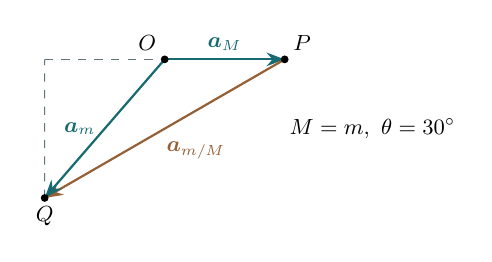
\begin{tikzpicture}[scale=.88,transform shape]
\coordinate (O) at (0,0);
\coordinate (P) at (1.73205,0);
\coordinate (Q) at (-1.73205,-2);
\draw[motion] (O)--(P) node[midway,above] {$\vect a_M$};
\draw[force] (P)--(Q) node[pos=.53,below right] {$\vect a_{m/M}$};
\draw[motion] (O)--(Q) node[midway,left] {$\vect a_m$};
\draw[guide] (Q)--(-1.73205,0);
\draw[guide] (-1.73205,0)--(O);
\fill (O) circle(1.6pt) node[above left] {$O$};
\fill (P) circle(1.6pt) node[above right] {$P$};
\fill (Q) circle(1.6pt) node[below] {$Q$};
\node at (3,-1) {$M=m,\ \theta=30^\circ$};
\end{tikzpicture}
\figcaption{变图2.4V2\quad 相对加速度沿下坡，和斜面加速度相加得到木块对地加速度。}
\end{minipage}\end{center}
\item 斜面体底面与地面平稳接触，地面静摩擦系数为 $\nu$。求维持静止的条件。固定斜面时，木块的法向加速度为零，$N=mg\cos\theta$。变图2.4V3 的接触力 $-\vect N$ 具有向右的 $N\sin\theta$ 和向下的 $N\cos\theta$。因此地面对斜面体的静摩擦向左，大小 $f_g=N\sin\theta$，地面支持力 $N_g=Mg+N\cos\theta$。由 $f_g\leq\nu N_g$ 得
\[
\nu\geq\frac{m\sin\theta\cos\theta}{M+m\cos^2\theta}.
\]
图中取 $M=m,\theta=45^\circ$，$f_g=mg/2$、$N_g=3mg/2$，所需最小系数为 $1/3$。
\begin{center}\begin{minipage}{.98\linewidth}\centering
\begin{tikzpicture}[scale=.88,transform shape]
\draw[object] (-2.2,0)--(2.2,0);
\draw[object,fill=rulegray!15] (-1.6,0)--(1.6,3.2)--(1.6,0)--cycle;
\coordinate (C) at (.4,2);
\draw[force] (C)--(1.2,1.2) node[pos=.59,above right] {$-\vect N$};
\draw[force] (.53,1.07)--(.53,-.53) node[below] {$Mg$};
\draw[force] (1.16,0)--(1.16,2.4) node[above] {$N_g$};
\draw[force] (1.16,0)--(.36,0) node[midway,below] {$f_g$};
\fill (C) circle(1.6pt) node[above left] {$C$};
\node at (-1.4,-.65) {斜面体静止};
\end{tikzpicture}
\figcaption{变图2.4V3\quad 地面的水平摩擦平衡接触力的水平分量。}
\end{minipage}\end{center}
\item 取 $M=m,\theta=45^\circ$，求加速度和支持力。此时 $D=3m/2$，代入法向力和水平方程得 $N=\sqrt2mg/3$、$a_M=g/3$、$a_x=-g/3$。木块的竖直合力为 $N/\sqrt2-mg=-2mg/3$，故 $a_y=-2g/3$。变图2.4V4 把 $\vect N$ 与重力合成向左下的木块合力。它的水平分量与斜面体的合力大小相等、方向相反。用 $a_x-a_M=-2g/3$ 及 $a_y=-2g/3$ 代入式(2)，相对加速度的法向分量为零。
\begin{center}\begin{minipage}{.98\linewidth}\centering
\begin{tikzpicture}[scale=.88,transform shape]
\begin{scope}
\coordinate (O) at (0,0);
\coordinate (P) at (-.9,.9);
\coordinate (Q) at (-.9,-1.8);
\draw[force] (O)--(P) node[above left] {$\vect N$};
\draw[force] (P)--(Q) node[pos=.46,left] {$m\vect g$};
\draw[motion] (O)--(Q) node[pos=.68,right] {$m\vect a_m$};
\node[above] at (0,1.2) {木块};
\draw[guide] (Q)--(0,-1.8)--(O);
\end{scope}
\begin{scope}[xshift=3.9cm]
\draw[object] (-.55,-.35) rectangle (.55,.35);
\draw[force] (0,0)--(.9,0) node[right] {$Ma_M$};
\node[above] at (0,1.2) {斜面体};
\end{scope}
\end{tikzpicture}
\figcaption{变图2.4V4\quad 等质量时两个物体的水平合力大小相等，方向相反。}
\end{minipage}\end{center}
\end{enumerate}

\clearpage

\pdfbookmark[2]{第 5 题 旋转球壳中木块的摩擦条件与稳定性}{q5}

\section*{第 5 题\quad 旋转球壳中木块的摩擦条件与稳定性}

\tagline{M-02-05}

半径 $R=0.5\,\mathrm m$ 的空心球壳绕竖直直径匀速转动。内壁上的小木块可看作质点，位于距球壳最低点 $h=R/2$ 的高度，随壳共转。取 $g=9.8\,\mathrm{m/s^2}$。
\begin{enumerate}
\item 当 $\omega=5\,\mathrm{s^{-1}}$ 时，至少需要多大的静摩擦系数？
\item 当 $\omega=8\,\mathrm{s^{-1}}$ 时，维持共转的条件是什么？
\item 分别讨论木块位置、角速度发生微小改变后能否继续共转。区分静摩擦有余量和恰好临界的情形，说明仅由这些条件能否断言木块必定返回原位置。
\end{enumerate}

\begin{center}\begin{minipage}{\linewidth}\centering\begin{tikzpicture}

\draw[object] (0,0) circle(2.4);\draw[guide] (0,-2.4)--(0,2.4);
\coordinate (B) at (2.078,-1.2);\draw[object] (0,0)--(B);\draw[guide] (0,-1.2)--(B);
\fill (B) circle(2.5pt);\node[right] at (B) {木块};\node[left] at (0,0) {$O$};
\draw (0,-.7) arc(-90:-30:.7);\node at (.55,-.85) {$\theta$};
\draw[thin,<->] (2.75,-2.4)--(2.75,-1.2) node[midway,right] {$h=R/2$};
\draw[guide] (0,-2.4)--(2.75,-2.4);\draw[guide] (B)--(2.75,-1.2);
\draw[motion] (-.45,2.05) arc(150:-120:.5 and .18) node[left] {$\omega$};

\end{tikzpicture}
\figcaption{图 2.5\quad 高度从球壳最低点量起，$h=R(1-\cos\theta)$，本题 $\theta=60^\circ$。}
\end{minipage}\end{center}

\Needspace{5\baselineskip}

\pdfbookmark[3]{题型定位}{q5-h0}

\subsection*{题型定位}

旋转球壳内壁的共转条件。先求有符号摩擦比，再根据位置和转速变化判断材料还有多少余量。静止共转、初始滑动方向和后续运动分别由相应的力学条件决定。

\Needspace{5\baselineskip}

\pdfbookmark[3]{知识点}{q5-h1}

\subsection*{知识点}

水平向心加速度、球面法向与经线方向、静摩擦上限和有符号比 $\eta=f/N$。绝对值的增减由 $\eta$ 的符号和导数共同决定。调速过程中还有周向摩擦，应和经线摩擦作矢量合成。


\Needspace{5\baselineskip}

\pdfbookmark[3]{物理图像}{q5-h2}

\subsection*{物理图像}

图2.5 从球壳最低点量高度，$h=R(1-\cos\theta)$，所以
\[
\cos\theta=\frac12,\qquad \theta=60^\circ.
\]
木块随壳绕竖直轴作水平圆周运动。解图2.5A 左图在低转速下画出向上的经线摩擦，右图在高转速下画出向下摩擦，方向由 $g-R\omega^2\cos\theta$ 的符号决定。解图2.5B 用水平线表示材料系数，纵坐标是 $|\eta|$，曲线落在线下的区间给出可共转的位置。

\Needspace{5\baselineskip}

\pdfbookmark[3]{解题入口}{q5-h3}

\subsection*{解题入口}

从题图由 $h=R(1-\cos\theta)$ 求角度。按图2.5A 在地面系列 $N\sin\theta-f\cos\theta=mR\omega^2\sin\theta$、$N\cos\theta+f\sin\theta=mg$。由两式先求 $f/m,N/m$，再算 $\eta=f/N$。扰动时，有严格余量的一组由连续性判断，恰临界的一组分别考察 $\partial_\theta\eta$ 与 $\partial_\omega\eta$。若 $\eta<0$，$|\eta|$ 的变化方向与 $\eta$ 的变化方向相反。

\Needspace{5\baselineskip}

\pdfbookmark[3]{标准解法}{q5-h4}

\subsection*{标准解法}

图 2.5 中高度从最低点量起，$h=R(1-\cos\theta)$。由 $h=R/2$ 得 $\theta=60^\circ$，水平圆周半径为 $R\sin\theta$。小木块做水平圆周运动，加速度朝向转轴，大小为 $R\omega^2\sin\theta$。解图2.5A 在两幅受力图下方分别画出向轴的加速度。

规定摩擦 $f$ 沿经线上行为正。按解图 2.5A 的两幅受力图，地面系的水平与竖直方程是
\[
N\sin\theta-f\cos\theta=mR\omega^2\sin\theta,
\qquad N\cos\theta+f\sin\theta=mg.
\]
\begin{center}\begin{minipage}{\linewidth}\centering\begin{tikzpicture}

\begin{scope}
\fill (0,0) circle(2pt);\draw[force] (0,0)--(-1.76607,1.01964) node[above left] {$N$};
\draw[force] (0,0)--(0.21960,0.38036) node[above right] {$f>0$};\draw[force] (0,0)--(0,-1.4) node[below] {$mg$};
\draw[motion] (0,-2)--(-0.92015,-2) node[left] {$\vect a$};\node at (0,2.55) {$\omega=5\,\mathrm{s^{-1}}$};
\end{scope}
\begin{scope}[xshift=5.8cm]
\fill (0,0) circle(2pt);\draw[force] (0,0)--(-3.57545,2.06429) node[above left] {$N$};
\draw[force] (0,0)--(-0.38353,-0.66429) node[below left] {$f<0$};\draw[force] (0,0)--(0,-1.4) node[below] {$mg$};
\draw[motion] (0,-2)--(-2.35559,-2) node[left] {$\vect a$};\node at (0,2.55) {$\omega=8\,\mathrm{s^{-1}}$};
\end{scope}

\end{tikzpicture}
\figcaption{解图 2.5A\quad 两种转速下的受力和向轴加速度。两幅图的重力箭头等长，支持力与摩擦力按各自大小绘出。}
\end{minipage}\end{center}
消元得到
\[
f=m(g-R\omega^2\cos\theta)\sin\theta,
\qquad N=m(g\cos\theta+R\omega^2\sin^2\theta).
\]
用有符号比值 $\eta=f/N$ 记录方向，材料静摩擦系数记为非负的 $\mu_s$，则
\[
\boxed{\eta=\frac{(g-R\omega^2\cos\theta)\sin\theta}
{g\cos\theta+R\omega^2\sin^2\theta}},\qquad \mu_s\geq|\eta|.
\]
\subsubsection*{两种转速的数值与方向}
$R=0.5\,\mathrm m$、$g=9.8\,\mathrm{m/s^2}$、$\theta=60^\circ$。当 $\omega=5\,\mathrm{s^{-1}}$ 时，
\[
\frac Nm=4.9+12.5\times\frac34=14.275\,\mathrm{m/s^2},
\quad \frac fm=(9.8-6.25)\frac{\sqrt3}{2}=3.0744\,\mathrm{m/s^2}.
\]
故 $\boxed{\mu_s\geq0.2154}$，摩擦向上。$\omega=8\,\mathrm{s^{-1}}$ 时，
\[
\frac Nm=4.9+32\times\frac34=28.9\,\mathrm{m/s^2},
\quad \frac fm=(9.8-16)\frac{\sqrt3}{2}=-5.3694\,\mathrm{m/s^2}.
\]
故 $\boxed{\mu_s\geq0.1858}$，摩擦向下。$f/N<0$ 对应经线向下的摩擦，所需的最小材料系数取 $|f/N|$。零摩擦的分界转速为 $\sqrt{g/(R\cos\theta)}\approx6.261\,\mathrm{s^{-1}}$。

\subsubsection*{位置与转速改变后的静摩擦条件}
如果 $\mu_s>|\eta|$，摩擦有严格余量，连续性保证足够小的角度或转速改变后仍可共转。这里比较的是新共转状态所需的摩擦，扰动后的木块可以保持在新位置。

材料恰在临界时，新的 $|\eta|$ 增大便会超过上限，减小则留下余量。令 $u=R\omega^2/g$、$D=\cos\theta+u\sin^2\theta$，则 $\eta=(1-u\cos\theta)\sin\theta/D$。记 $A=(1-u\cos\theta)\sin\theta$。对角度求导，有 $A_\theta=\cos\theta-u(\cos^2\theta-\sin^2\theta)$、$D_\theta=-\sin\theta+2u\sin\theta\cos\theta$，商法则的分子为 $A_\theta D-AD_\theta$。对 $u$ 求导，分子是 $-\cos\theta\sin\theta\,D-A\sin^2\theta=-\sin\theta$。再乘 $du/d\omega=2R\omega/g$，整理得
\[
\frac{\partial\eta}{\partial\theta}
=\frac{1-u\cos\theta+u^2\sin^2\theta}{D^2},
\qquad \frac{\partial\eta}{\partial\omega}
=-\frac{2R\omega\sin\theta}{gD^2}.
\]
在本题两个状态处，第一导数为正、第二导数为负。沿球面经线上移时，$\theta$ 增大，在解图2.5B中向右读。第一种状态 $\eta>0$，第二种状态 $\eta<0$，因此两条 $|\eta|$ 曲线在该处的斜率一正一负。
\begin{center}\begin{minipage}{\linewidth}\centering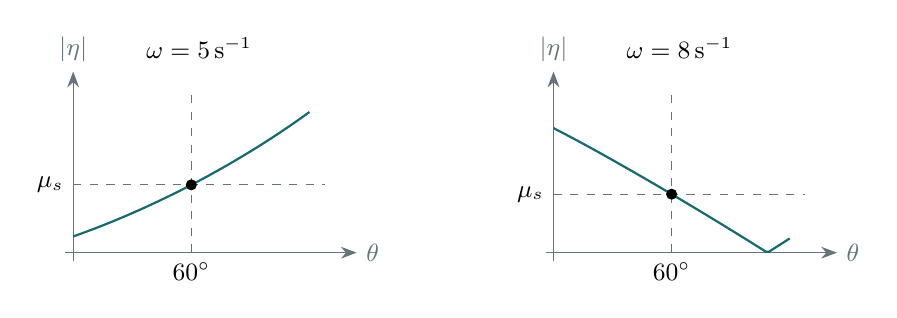
\begin{tikzpicture}

\begin{scope}
\draw[axis] (-.1,0)--(3.6,0) node[right] {$\theta$};\draw[axis] (0,-.1)--(0,2.3) node[above] {$|\eta|$};
\draw[traj,domain=45:75,samples=80] plot({(\x-45)/10},{4*abs((1-1.2755102*cos(\x))*sin(\x)/(cos(\x)+1.2755102*sin(\x)*sin(\x)))});
\draw[guide] (1.5,0)--(1.5,2);\draw[guide] (0,.8616)--(3.2,.8616);
\fill (1.5,.8616) circle(2pt);\node[below] at (1.5,0) {$60^\circ$};\node[left] at (0,.8616) {$\mu_s$};
\node at (1.6,2.6) {$\omega=5\,\mathrm{s^{-1}}$};
\end{scope}
\begin{scope}[xshift=6.1cm]
\draw[axis] (-.1,0)--(3.6,0) node[right] {$\theta$};\draw[axis] (0,-.1)--(0,2.3) node[above] {$|\eta|$};
\draw[traj,domain=45:75,samples=80] plot({(\x-45)/10},{4*abs((1-3.2653061*cos(\x))*sin(\x)/(cos(\x)+3.2653061*sin(\x)*sin(\x)))});
\draw[guide] (1.5,0)--(1.5,2);\draw[guide] (0,.7432)--(3.2,.7432);
\fill (1.5,.7432) circle(2pt);\node[below] at (1.5,0) {$60^\circ$};\node[left] at (0,.7432) {$\mu_s$};
\node at (1.6,2.6) {$\omega=8\,\mathrm{s^{-1}}$};
\end{scope}

\end{tikzpicture}
\figcaption{解图 2.5B\quad 固定转速的位置扰动。水平虚线取 $60^\circ$ 位置的临界系数，虚线下方的曲线对应可继续共转的位置。}
\end{minipage}\end{center}
\begin{center}
\begin{tabular}{@{}lll@{}}\toprule
微小改变 & $\omega=5\,\mathrm{s^{-1}}$ & $\omega=8\,\mathrm{s^{-1}}$\\\midrule
位置上移 & 需求增大，开始下滑 & 需求减小，可在新位置共转\\
位置下移 & 需求减小，可在新位置共转 & 需求增大，开始上滑\\
转速升高 & 需求减小，可继续共转 & 需求增大，开始上滑\\
转速降低 & 需求增大，开始下滑 & 需求减小，可继续共转\\\bottomrule
\end{tabular}\end{center}
表中“开始滑动”的方向，由超出最大静摩擦后仍未平衡的经线分力确定。例如第一种状态上移后，所需向上摩擦超过材料上限，剩余合力向下。

表中的共转情形是把木块在新位置无相对速度地放开。材料有余量时，木块可以停留在该处。若放开时已有相对速度，或静摩擦达到上限后开始滑动，后续轨迹由扰动速度、动摩擦规律和周向运动共同决定。
\subsubsection*{经线上的摩擦方向与大小}
局部斜率给出 $60^\circ$ 附近的增减。沿经线从底部移向赤道，$\sin\theta$ 增大，$\cos\theta$ 减小，分子中的 $1-u\cos\theta$ 可以由负转正。两种转速的过零位置因此不同。
把表中每个角度代入 $\eta(\theta,\omega)$。正值指向经线上方，负值指向经线下方，相应材料系数取该数的绝对值。
\begin{center}
\begin{tabular}{@{}rrrrrrrr@{}}\toprule
$\theta$ & $0^\circ$ & $15^\circ$ & $30^\circ$ & $45^\circ$ & $60^\circ$ & $75^\circ$ & $90^\circ$\\\midrule
$\eta(\theta,5)$ & 0 & $-0.0571$ & $-0.0441$ & $0.0516$ & $0.2154$ & $0.4466$ & $0.7840$\\
$\eta(\theta,8)$ & 0 & $-0.4706$ & $-0.5432$ & $-0.3956$ & $-0.1858$ & $0.0453$ & $0.3063$\\\bottomrule
\end{tabular}
\end{center}
在 $\theta=0$ 的最低点，重力与向轴加速度的切向投影都为零，$\eta=0$。当 $\theta\to90^\circ$，重力全在切向，支持力全用于向心加速，于是 $\eta\to g/(R\omega^2)$。
因此这两行末值分别是$9.8/12.5$和$9.8/32$。
有符号需求在$\cos\theta=1/u$处过零，过零前后摩擦方向互换。
在$60^\circ$附近，第一行的$\eta$为正且随角度增加，
第二行的$\eta$为负且随角度增加；转为绝对值以后，两条需求曲线的升降方向相反，
与解图2.5B相符。

以图2.5B 左图为例，上移使向上摩擦需求超过临界线，静摩擦取到上限后，剩余分力沿经线向下。下移让需求落到临界线下方，木块可以静止在新位置。右图的临界曲线在 $60^\circ$ 处斜率反号，下移使所需向下摩擦超过上限，剩余分力向上。图中每一点的纵坐标都除以该位置的支持力 $N$，它与摩擦力一起随位置改变。

\subsubsection*{实际调速过程还需要周向摩擦}
前面的转速比较针对调整前、后两个匀速共转状态。
若在有限时间内改变球壳角速度，同时要求木块始终留在同一纬度并随壳转动，
还需要周向摩擦$f_\varphi=mR\sin\theta\,\dot\omega$，
它负责角速度变化引起的周向加速度。
经线所需摩擦仍为$f_\theta=m(g-R\omega^2\cos\theta)\sin\theta$，
经线和周向两分量正交，合成的静摩擦条件为
\[
\sqrt{f_\theta^2+f_\varphi^2}\leq\mu_sN,
\qquad N=m(g\cos\theta+R\omega^2\sin^2\theta).
\]
等价地，令$D=\cos\theta+u\sin^2\theta$，
\[
\eta^2+
\left(\frac{R\sin\theta\,\dot\omega}{gD}\right)^2
\leq\mu_s^2.
\]
在 $\dot\omega=0$ 的匀速阶段，条件化为 $|\eta|\leq\mu_s$。调速时可供周向分量使用的余量为 $N\sqrt{\mu_s^2-\eta^2}$。在经线摩擦恰达上限的时刻，这一余量为零。由合摩擦式可为两个匀速状态之间的调速过程选取允许的角加速度。


\Needspace{5\baselineskip}

\pdfbookmark[3]{关键洞察}{q5-h5}

\subsection*{关键洞察}

摩擦方向由 $\eta$ 的正负给出，材料能否维持共转由 $|\eta|\leq\mu_s$ 给出。系数有余量时，木块可以静止在附近的新位置。超出上限时，剩余经线分力给出初始滑动方向，之后的运动由滑动摩擦和速度决定。

\Needspace{5\baselineskip}

\pdfbookmark[3]{易错点}{q5-h6}

\subsection*{易错点}

\begin{itemize}
\item $\eta$ 可取负值，材料系数始终非负。负支的需求大小用 $-\eta$ 表示。
\item 图2.5 的 $h$ 从壳底量起，$h/R=1/2$ 对应下半球的 $60^\circ$。
\item 静摩擦达到上限时取等号。严格低于上限时，连续的小变化仍可能保持共转。
\item 位移扰动后若已带有相对速度，应把动摩擦与周向运动写进后续方程。
\end{itemize}

\Needspace{5\baselineskip}

\pdfbookmark[3]{课堂讲解建议}{q5-h7}

\subsection*{课堂讲解建议}

先遮住图2.5A 的两支摩擦箭头，让学生分别计算 $g-R\omega^2\cos\theta$ 并画出方向。再指向图2.5B 左、右两曲线，问“同样把木块上移，为什么两种转速的材料需求一增一减？”答题时先说两种 $\eta$ 同随角度增加，再分别取正支与负支的绝对值。用变图2.5V4 把材料线抬到 $0.25$，请学生读出两点都在下方，解释木块可停留在附近位置。最后追问“调速时沿周向也要加速，哪支摩擦箭头还会出现？”由 $f_\varphi=mR\sin\theta\,\dot\omega$ 画出垂直经线的另一分量。

\Needspace{5\baselineskip}

\pdfbookmark[3]{变式训练}{q5-h8}

\subsection*{变式训练}

\begin{enumerate}
\item 在 $h=R/2$ 的纬圈上求零摩擦角速度。由竖直平衡得 $N\cos60^\circ=mg$，水平分量满足 $N\sin60^\circ=mR\omega_0^2\sin60^\circ$。消去 $N$ 得
\[
\omega_0=\sqrt{\frac{g}{R\cos60^\circ}}=\sqrt{39.2}\,\mathrm{s^{-1}}\simeq 6.261\,\mathrm{s^{-1}}.
\]
变图2.5V1 从转动系看同一状态。离心力向外，重力向下，两箭头的合力恰沿球面半径向外，球壁的支持力沿反向与它平衡，切向所需摩擦为零。
\begin{center}\begin{minipage}{.98\linewidth}\centering
\begin{tikzpicture}[scale=.88,transform shape]
\coordinate (P) at (0,0);
\coordinate (A) at (2.07846,0);
\coordinate (Q) at (2.07846,-1.2);
\draw[force] (P)--(A) node[midway,above] {$mR\omega_0^2\sin\theta$};
\draw[force] (A)--(Q) node[midway,right] {$mg$};
\draw[guide] (P)--(Q) node[midway,below left] {沿半径向外};
\draw[force] (P)--(-2.07846,1.2) node[above left] {$N$};
\fill (P) circle(1.6pt) node[above left] {$P$};
\node at (1.3,1) {$f=0$};
\end{tikzpicture}
\figcaption{变图2.5V1\quad 转动系中重力和离心力合成后沿半径向外，支持力与它平衡。}
\end{minipage}\end{center}
\item 改为 $\theta=45^\circ$，求两个转速的最小材料系数和摩擦方向。此时 $\sin\theta=\cos\theta=1/\sqrt2$，令 $u=R\omega^2/g$，有
\[
\eta=\frac{(1-u/\sqrt2)/\sqrt2}{1/\sqrt2+u/2}.
\]
在 $\omega=5\,\mathrm{s^{-1}}$ 时 $u=12.5/9.8$，得 $\eta=0.05157$，最小系数为 $0.05157$，摩擦沿经线上方。在 $\omega=8\,\mathrm{s^{-1}}$ 时 $u=32/9.8$，得 $\eta=-0.39557$，最小系数为 $0.39557$，摩擦沿经线下方。变图2.5V2 的两点分列横轴两侧。图上零点给这一纬圈的零摩擦转速 $\sqrt{g/(R\cos45^\circ)}$。
\begin{center}\begin{minipage}{.98\linewidth}\centering
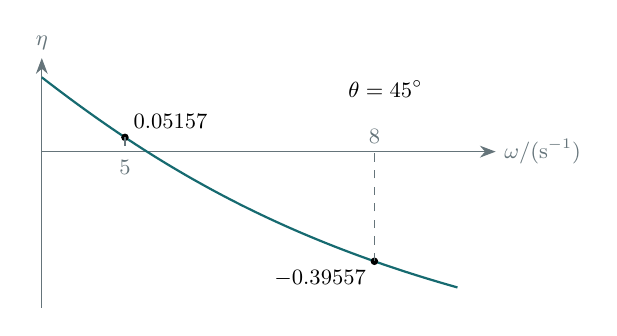
\begin{tikzpicture}[scale=.88,transform shape]
\draw[axis] (0,0)--(6.55,0) node[right] {$\omega/(\mathrm{s^{-1}})$};
\draw[axis] (0,-2.25)--(0,1.35) node[above] {$\eta$};
\draw[traj,domain=4:9,samples=100] plot({1.2*(\x-4)},{4*(1-.7071068*\x^2/19.6)*.7071068/(.7071068+.5*\x^2/19.6)});
\fill (1.2,.20627) circle(1.55pt) node[above right] {$0.05157$};
\fill (4.8,-1.58229) circle(1.55pt) node[below left] {$-0.39557$};
\draw[guide] (1.2,.20627)--(1.2,0) node[below] {$5$};
\draw[guide] (4.8,-1.58229)--(4.8,0) node[above] {$8$};
\node[above right] at (4.3,.66) {$\theta=45^\circ$};
\end{tikzpicture}
\figcaption{变图2.5V2\quad 两个转速分居零摩擦点两侧，所需摩擦方向相反。}
\end{minipage}\end{center}
\item 固定 $u=R\omega^2/g$，求有符号比的极值位置。令 $\partial_\theta\eta=0$，因分母为正，只需解 $1-u\cos\theta+u^2\sin^2\theta=0$。对 $u>0$，置 $c=\cos\theta$，得
\[
u^2c^2+uc-(1+u^2)=0,\qquad
c=\frac{-1+\sqrt{5+4u^2}}{2u}.
\]
二次式随 $c\in(0,1)$ 严格增加，在 $c=0$ 为负，在 $c=1$ 等于 $u-1$。所以 $u>1$ 时才有下半球内部根，$\eta$ 在该点由减转增，取得极小值。$u=0$ 时 $\eta=\tan\theta$ 单调增加。变图2.5V3 取 $u=2$，极小点约在 $26.4^\circ$。若求的是 $|\eta|$，还要把 $\eta=0$ 的尖点列入候选，图中它在 $60^\circ$。
\begin{center}\begin{minipage}{.98\linewidth}\centering
\begin{tikzpicture}[scale=.88,transform shape]
\draw[axis] (0,0)--(6.65,0) node[right] {$\theta$};
\draw[axis] (0,-1.5)--(0,2.45) node[above] {$\eta$};
\draw[traj,domain=0:90,samples=130] plot({\x/15},{4*(1-2*cos(\x))*sin(\x)/(cos(\x)+2*sin(\x)^2)});
\fill (1.76058,-1.09021) circle(1.65pt) node[below right] {极小点};
\draw[guide] (1.76058,-1.09021)--(1.76058,0) node[above] {$26.4^\circ$};
\fill (4,0) circle(1.55pt) node[below right] {$60^\circ$};
\fill (6,2) circle(1.55pt) node[right] {$1/2$};
\node[above right] at (4.2,.9) {$u=2$};
\end{tikzpicture}
\figcaption{变图2.5V3\quad 有符号比先减后增，在过零后变成向上的摩擦。}
\end{minipage}\end{center}
\item 材料系数为 $\mu_s=0.25$ 时，讨论两种转速和小扰动。$\theta=60^\circ$ 时的 $|\eta|$ 分别约为 $0.21537$ 和 $0.18579$，小于材料系数。变图2.5V4 的两个点都在阴影带内，连续性给每点附近的一段可共转纬圈。保持高度不变而改变转速时，把 $\eta(\cos\theta+u\sin^2\theta)=(1-u\cos\theta)\sin\theta$ 两端含 $u$ 的项合并，得
\[
u=\frac{\sin\theta-\eta\cos\theta}{\sin\theta\cos\theta+\eta\sin^2\theta}.
\]
这里 $\eta$ 随 $u$ 递减，将 $\eta=0.25$ 和 $-0.25$ 分别代入，得
\[
1.1942\lesssim R\omega^2/g\lesssim 4.0366,
\qquad
4.838\,\mathrm{s^{-1}}\lesssim\omega\lesssim8.895\,\mathrm{s^{-1}}.
\]
两个题定转速都在区间内部。给木块一个小位移后，若在新位置无相对速度地放开，静摩擦可使它在那里保持共转。若扰动给予相对速度，后续运动由速度与动摩擦决定。
\begin{center}\begin{minipage}{.98\linewidth}\centering
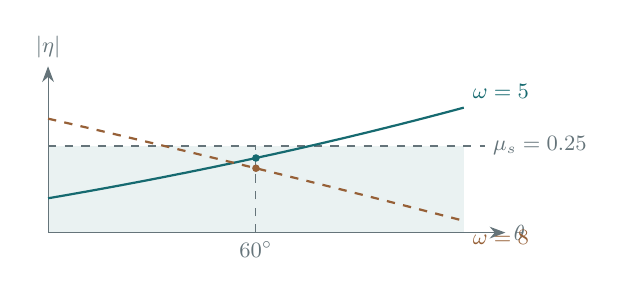
\begin{tikzpicture}[scale=.88,transform shape]
\fill[accent!9] (0,0) rectangle (6,1.25);
\draw[axis] (0,0)--(6.6,0) node[right] {$\theta$};
\draw[axis] (0,0)--(0,2.4) node[above] {$|\eta|$};
\draw[guide] (0,1.25)--(6.3,1.25) node[right] {$\mu_s=0.25$};
\draw[traj,domain=50:70,samples=100] plot({.3*(\x-50)},{5*abs((1-1.2755102*cos(\x))*sin(\x)/(cos(\x)+1.2755102*sin(\x)^2))}) node[above right] {$\omega=5$};
\draw[guide,thick,color=warm,domain=50:70,samples=100] plot({.3*(\x-50)},{5*abs((1-3.2653061*cos(\x))*sin(\x)/(cos(\x)+3.2653061*sin(\x)^2))}) node[below right] {$\omega=8$};
\draw[guide] (3,0)--(3,1.25) node[pos=0,below] {$60^\circ$};
\fill[accent] (3,1.07684) circle(1.55pt);
\fill[warm] (3,.92895) circle(1.55pt);
\end{tikzpicture}
\figcaption{变图2.5V4\quad 两条曲线在题定位置都低于材料系数，附近有一段可共转的纬圈。}
\end{minipage}\end{center}
\end{enumerate}

\clearpage

\pdfbookmark[2]{第 6 题 反向滚轴上的钢件匀速推动}{q6}

\section*{第 6 题\quad 反向滚轴上的钢件匀速推动}

\tagline{M-02-06}

质量 $m=20\,\mathrm{kg}$ 的对称钢件架在两个相同的平行长直滚轴上。滚轴轴线水平，半径 $r=0.025\,\mathrm m$，以角速度 $\omega=40\,\mathrm{rad/s}$ 反向转动，接触处的表面速度大小均为 $\omega r$，方向水平且相反。钢件与滚轴间的滑动摩擦系数 $\mu=0.20$。要使钢件沿滚轴轴线以 $v_0=0.050\,\mathrm{m/s}$ 匀速运动，需施加多大的轴向水平力 $F$？取 $g=10\,\mathrm{m/s^2}$。

\begin{center}\begin{minipage}{\linewidth}\centering\begin{tikzpicture}

\draw[object] (0,0) ellipse(.45 and .22);\draw[object] (0,0)--(0,3);\draw[object] (.45,0)--(.45,3);\draw[object] (-.45,0)--(-.45,3);\draw[object] (0,3) ellipse(.45 and .22);
\draw[object] (3,0) ellipse(.45 and .22);\draw[object] (3,0)--(3,3);\draw[object] (3.45,0)--(3.45,3);\draw[object] (2.55,0)--(2.55,3);\draw[object] (3,3) ellipse(.45 and .22);
\filldraw[object,fill=white] (-.7,.9) rectangle (3.7,2);\node at (1.5,1.45) {钢件};
\draw[motion] (0,2.6)--(-1.2,2.6) node[left] {$\omega r$};\draw[motion] (3,2.6)--(4.2,2.6) node[right] {$\omega r$};
\draw[motion] (1.5,2)--(1.5,3.6) node[above] {$v_0,F$};\node at (1.5,-.6) {俯视图：图中上下方向沿滚轴轴线};

\end{tikzpicture}
\figcaption{图 2.6\quad 两接触处的横向表面速度相反。}
\end{minipage}\end{center}

\Needspace{5\baselineskip}

\pdfbookmark[3]{题型定位}{q6-h0}

\subsection*{题型定位}

两个滑动接触的摩擦方向由局部速度差确定。先在俯视图中写两处相对速度，再分解两个摩擦力，用轴向匀速条件求外力。

\Needspace{5\baselineskip}

\pdfbookmark[3]{知识点}{q6-h1}

\subsection*{知识点}

每个滚轴分担一半重力。滑动摩擦大小为$\mu N_i$，方向沿钢件相对该处表面速度的反向。两处相对速度的横向分量相反，轴向分量相同。图2.6A上的两个速度三角形因此互为镜像，摩擦力的轴向分量相加。


\Needspace{5\baselineskip}

\pdfbookmark[3]{物理图像}{q6-h2}

\subsection*{物理图像}

题图中钢件沿滚轴轴线移动，两个滚轴顶端分别向左、向右运动。钢件相对左滚轴的速度斜向右上，相对右滚轴的速度斜向左上。沿解图2.6A将两条相对速度箭头各转$180^\circ$，便得到两处摩擦方向。它们的横向作用抵消，轴向作用同向指向后方。

\Needspace{5\baselineskip}

\pdfbookmark[3]{解题入口}{q6-h3}

\subsection*{解题入口}

在俯视平面取$x$横跨滚轴、$y$沿滚轴轴线。钢件速度为$(0,v_0)$。右、左滚轴表面速度分别为$(w,0)$、$(-w,0)$，用钢件速度分别减去这两个表面速度，得到两处的相对速度。它们大小相同，可用共同的$V=\sqrt{w^2+v_0^2}$归一化。乘上$-\mu mg/2$后相加，用外力平衡结果。若用投影角法，先在图2.6A标出相对速度与$y$轴的夹角，再取其余弦。

\Needspace{5\baselineskip}

\pdfbookmark[3]{标准解法}{q6-h4}

\subsection*{标准解法}

取滚轴轴向为 $y$，钢件运动方向为 $+y$，横跨两轴的方向为 $x$。两轴顶部表面速度大小均为 $w=\omega r$，方向分别为 $+x$、$-x$。接触摩擦反向于钢件相对各滚轴表面的速度。
\begin{center}\begin{minipage}{\linewidth}\centering\begin{tikzpicture}

\begin{scope}
\draw[axis] (-1.6,0)--(1.8,0) node[right] {$x$};\draw[axis] (0,-1.6)--(0,1.6) node[above] {$y$};
\draw[motion] (0,0)--(1.3,.6) node[right] {$\vect v_{\mathrm{rel},2}$};\draw[force] (0,0)--(-1.3,-.6) node[left] {$\vect f_2$};
\draw[guide] (1.3,0)--(1.3,.6);\node[below] at (.65,0) {$\omega r$};\node[right] at (1.3,.25) {$v_0$};
\node[below] at (0,-1.7) {左滚轴（2）};
\end{scope}
\begin{scope}[xshift=6cm]
\draw[axis] (-1.6,0)--(1.8,0) node[right] {$x$};\draw[axis] (0,-1.6)--(0,1.6) node[above] {$y$};
\draw[motion] (0,0)--(-1.3,.6) node[left] {$\vect v_{\mathrm{rel},1}$};\draw[force] (0,0)--(1.3,-.6) node[right] {$\vect f_1$};
\node[below] at (0,-1.7) {右滚轴（1）};
\end{scope}

\end{tikzpicture}
\figcaption{解图 2.6A\quad 摩擦方向由相对滑动决定；沿轴的速度分量在图中画长，便于读出两次投影。}
\end{minipage}\end{center}
解图 2.6A 的速度三角形给出
\[
\vect v_{\mathrm{rel},1}=(-w,v_0),\qquad
\vect v_{\mathrm{rel},2}=(w,v_0),\qquad
V=\sqrt{w^2+v_0^2}.
\]
钢件对称放置、没有竖直加速度，两接触处支持力均为 $N_1=N_2=mg/2$。两摩擦力的大小是 $\mu mg/2$，方向分别沿相对速度的反向，因而
\[
\vect f_1=\frac{\mu mg}{2V}(w,-v_0),\qquad
\vect f_2=\frac{\mu mg}{2V}(-w,-v_0).
\]
解图2.6A中每个摩擦力都与本处的相对速度反向。沿轴的阻力只取各自箭头在$-y$方向的投影。

两式相加，横向分量抵消，轴向阻力相加：
\[
\vect f_1+\vect f_2=\left(0,-\frac{\mu mgv_0}{V}\right).
\]
匀速要求轴向合力为零，外力向 $+y$，大小为
\[
\boxed{F=\frac{\mu mgv_0}{\sqrt{(\omega r)^2+v_0^2}}
=\frac{\mu mg}{\sqrt{1+(\omega r/v_0)^2}}}.
\]
代入 $\omega r=40\times0.025=1.00\,\mathrm{m/s}$、$v_0=0.050\,\mathrm{m/s}$、$g=10\,\mathrm{m/s^2}$，得到
\[
F=\frac{0.20\times20\times10}{\sqrt{401}}
=1.9975\,\mathrm N\approx\boxed{2.0\,\mathrm N}.
\]
\subsubsection*{为何远小于普通水平面上的摩擦}
每处摩擦的大小为$\mu N_i$，沿轴向的分量取决于箭头与轴线的夹角。本题$w/v_0=20$，相对速度接近横向，摩擦也几乎横向，其轴向比例只有 $v_0/V\approx0.05$。当 $v_0\ll\omega r$ 时，$F\approx\mu mgv_0/(\omega r)$；若滚轴停止，$F\to\mu mg$。

能量分配也可逐项算出。钢件匀速，外推力功率为
\[P_{\rm push}=Fv_0=\frac{\mu mgv_0^2}{V}.\]
每个滚轴表面速度沿$x$向，所受摩擦的$x$分量大小为$\mu mgw/(2V)$，维持两滚轴转速的驱动功率因此为
\[P_{\rm motor}=2\frac{\mu mgw}{2V}w=\frac{\mu mgw^2}{V}.\]
相加得$P_{\rm push}+P_{\rm motor}=\mu mgV$，恰等于两个滑动接触的总耗散率。图2.6A中互相抵消的只是作用于钢件的横向合力，各滚轴处的摩擦功并未相消。

\subsubsection*{把相对速度方向换成投影角}
按图2.6的表面速度方向，右滚轴表面沿$x$正向运动，左滚轴沿$x$负向运动。
解图2.6A中，右滚轴编号1，左滚轴编号2。两处滑动速度分别由钢件速度减去相应的滚轴表面速度得到。
设每个相对速度与$y$正向夹角的大小为$\beta$，则
\[
\tan\beta=\frac{w}{v_0},\qquad
\cos\beta=\frac{v_0}{\sqrt{w^2+v_0^2}}.
\]
每处摩擦大小为$\mu mg/2$，其沿$y$负向的投影为
$(\mu mg/2)\cos\beta$，因此$F=2(\mu mg/2)\cos\beta$。
这个几何投影法与前面的两个力矢量相加完全一致。

当$v_0\to0$而滚轴仍转动，轴向投影趋于零，钢件可以不沿轴移动；
两接触处仍有横向相对滑动，摩擦耗散率趋于$\mu mgw$，
所需能量由滚轴驱动装置提供。当钢件和滚轴都静止时，接触处的摩擦由静摩擦平衡确定。


\Needspace{5\baselineskip}

\pdfbookmark[3]{关键洞察}{q6-h5}

\subsection*{关键洞察}

当$w$远大于$v_0$，两摩擦几乎沿横向。即使每个接触仍有大小$\mu mg/2$的摩擦，轴向推力只需补足其中很小的投影。变图2.6V3与V5分别改变两表面的方向和速率，可以从横向分量的大小判断外力是否还沿轴向。

\Needspace{5\baselineskip}

\pdfbookmark[3]{易错点}{q6-h6}

\subsection*{易错点}

\begin{itemize}
\item 速度三角形中的$w=\omega r$是表面线速度，$v_0$是钢件速度沿轴的分量。斜边给相对滑动速率。
\item 每处支持力为$mg/2$。用这一支持力分别求摩擦，再求合力。
\item 投影角从$+y$量起时，轴向比例为$v_0/V$，横向比例为$w/V$。
\item 轴向推力乘$v_0$给钢件的外推功率，滚轴驱动的功率取自滚轴表面速度及其摩擦的横向分量。
\end{itemize}

\Needspace{5\baselineskip}

\pdfbookmark[3]{课堂讲解建议}{q6-h7}

\subsection*{课堂讲解建议}

先只画解图2.6A右滚轴的速度三角形，让学生说明“钢件相对这一表面向哪里滑”。把摩擦箭头加上后，再用关于$y$轴的对称画出另一处。沿$x$、$y$分别投影，问“哪两个分量可以相加，哪些正好抵消”。用$v_0/V\simeq0.05$和两个$20\,\mathrm N$的摩擦箭头算出约$2\,\mathrm N$的推力。

然后让学生比较滚轴停止的变图2.6V2，指出此时两支摩擦全部沿轴。沿主解的能量计算，可用$Fv_0$和驱动装置的功率分别解释钢件平移、滚轴转动怎样给两个滑动接触供能。

\Needspace{5\baselineskip}

\pdfbookmark[3]{变式训练}{q6-h8}

\subsection*{变式训练}

\begin{enumerate}
\item \textbf{改变钢件速度。}保持滚轴表面速率$w>0$和接触载荷，求推力随轴向速度$v$的变化，并求推力达到$\mu mg/2$时的$v$。

每处滑动速度的大小为$\sqrt{w^2+v^2}$。两个摩擦力的轴向投影相加，得到
\[
F(v)=\frac{\mu mgv}{\sqrt{w^2+v^2}},\qquad
\frac{\dd F}{\dd v}=\frac{\mu mgw^2}{(w^2+v^2)^{3/2}}>0.
\]
变图2.6V1中，速度从零增加时，轴向投影逐渐占主导，推力由零趋近$\mu mg$。令$v/\sqrt{w^2+v^2}=1/2$，平方整理得$v=w/\sqrt3$，图中的水平虚线在此与曲线相交。
\begin{center}\begin{minipage}{.98\linewidth}\centering
\begin{tikzpicture}
\draw[axis] (0,0)--(6.65,0) node[right] {$v/w$};
\draw[axis] (0,0)--(0,3.25) node[above] {$F/(\mu mg)$};
\draw[traj,domain=0:4,samples=75] plot({1.5*\x},{2.65*\x/sqrt(1+\x^2)});
\draw[guide] (0,2.65)--(6,2.65);
\draw[guide] (0,1.325)--({1.5/sqrt(3)},1.325)--({1.5/sqrt(3)},0);
\fill ({1.5/sqrt(3)},1.325) circle(1.7pt);
\node[left] at (0,2.65) {$1$};\node[left] at (0,1.325) {$1/2$};
\node[below] at ({1.5/sqrt(3)},0) {$1/\sqrt3$};
\end{tikzpicture}
\figcaption{变图2.6V1\quad 轴向速度越大，滑动摩擦在轴向的投影越大}
\end{minipage}\end{center}

\item \textbf{滚轴停止转动。}钢件仍沿轴向以正速率滑动，求推力。

变图2.6V2中，接触处的相对速度都为$v\vect e_y$，摩擦力都沿$-y$。两滚轴各支承$mg/2$，每个摩擦力大小为$\mu mg/2$。匀速条件为$F-\mu mg/2-\mu mg/2=0$，故$F=\mu mg$，代入本题数据为$40\,\mathrm N$。
\begin{center}\begin{minipage}{.98\linewidth}\centering
\begin{tikzpicture}
\filldraw[object,fill=rulegray!25] (-2,-.65) rectangle (2,.65);
\node at (0,-.32) {钢件};
\draw[guide] (-1.3,-2)--(-1.3,2) (1.3,-2)--(1.3,2);
\fill (-1.3,0) circle(1.7pt);\fill (1.3,0) circle(1.7pt);
\draw[force] (-1.3,0)--(-1.3,-1.1) node[left] {$\mu mg/2$};
\draw[force] (1.3,0)--(1.3,-1.1) node[right] {$\mu mg/2$};
\draw[motion] (0,.12)--(0,2.32) node[above] {$F$};
\node[right] at (2.25,1.45) {$+y$沿轴线};
\end{tikzpicture}
\figcaption{变图2.6V2\quad 两处摩擦都沿轴线，推力的大小等于它们之和}
\end{minipage}\end{center}

\item \textbf{两滚轴同向转动。}两处表面均以$w\vect e_x$运动，钢件仍以$v\vect e_y$匀速平动，两处接触继续分担相同的支持力。求外力的两个水平分量。

两个相对速度都为$(-w,v)$。令$V=\sqrt{w^2+v^2}$，两摩擦同向，故$\vect f_1+\vect f_2=\mu mg(w,-v)/V$。变图2.6V3的外力箭头沿合摩擦的反向，
\[
\vect F=\frac{\mu mg}{V}(-w,v).
\]
外力的横向分量指向$-x$，轴向分量指向$+y$。外力大小为$\mu mg$，方向随$w/v$改变。
\begin{center}\begin{minipage}{.98\linewidth}\centering
\begin{tikzpicture}
\draw[axis] (-3.45,0)--(3.5,0) node[right] {$x$};
\draw[axis] (0,-1.7)--(0,2.35) node[above] {$y$};
\draw[motion] (0,0)--(-2.7,1.35) node[above left] {$\vect F$};
\draw[force] (0,0)--(2.7,-1.35) node[right] {$\vect f_1+\vect f_2$};
\draw[guide] (-2.7,0)--(-2.7,1.35)--(0,1.35);
\node[below] at (-1.35,0) {$F_x<0$};\node[right] at (0,1.35) {$F_y>0$};
\end{tikzpicture}
\figcaption{变图2.6V3\quad 同向表面运动使两个横向摩擦分量相加，图取$w=2v$}
\end{minipage}\end{center}

\item \textbf{滚轴转速加倍。}保持$v_0=0.050\,\mathrm{m/s}$与其余数据，求新推力。

角速度加倍后，表面速率由$1.00\,\mathrm{m/s}$增至$2.00\,\mathrm{m/s}$，比值$w/v_0$由20变为40。用同一个轴向投影式，
\[
F_2=\frac{40\,\mathrm N}{\sqrt{1+40^2}}=0.99969\ldots\,\mathrm N.
\]
变图2.6V4在横坐标1和2处给出两次推力。由于两个工况均有$w\gg v_0$，这一段近似服从$F\simeq\mu mgv_0/w$，所以新推力约为原先的一半。
\begin{center}\begin{minipage}{.98\linewidth}\centering
\begin{tikzpicture}
\draw[axis] (0,0)--(6.1,0) node[right] {$\omega_{\rm new}/\omega$};
\draw[axis] (0,0)--(0,3.6) node[above] {$F/\mathrm N$};
\draw[traj,domain=.55:2.8,samples=75] plot({2*\x},{.86*40/sqrt(1+400*\x^2)});
\draw[guide] (2,0)--(2,{.86*40/sqrt(401)})--(0,{.86*40/sqrt(401)});
\draw[guide] (4,0)--(4,{.86*40/sqrt(1601)})--(0,{.86*40/sqrt(1601)});
\fill (2,{.86*40/sqrt(401)}) circle(1.7pt);
\fill (4,{.86*40/sqrt(1601)}) circle(1.7pt);
\node[left] at (0,{.86*40/sqrt(401)}) {$2.0$};
\node[left] at (0,{.86*40/sqrt(1601)}) {$1.0$};
\node[below] at (2,0) {$1$};\node[below] at (4,0) {$2$};
\end{tikzpicture}
\figcaption{变图2.6V4\quad 在给定小轴速下，转速越大，轴向推力越小}
\end{minipage}\end{center}

\item \textbf{反向滚轴的表面速率不等。}已知接触载荷仍相等，表面速度分别为$+w_1\vect e_x$、$-w_2\vect e_x$，$w_1,w_2>0$。求维持钢件以$v\vect e_y$匀速运动的外力，$v>0$。

两处相对速度为$(-w_1,v)$、$(w_2,v)$。记$V_i=\sqrt{w_i^2+v^2}$。摩擦力分别为$(\mu mg/2)(w_1,-v)/V_1$和$(\mu mg/2)(-w_2,-v)/V_2$。将二者相加后反向，得到
\[
F_x=-\frac{\mu mg}{2}\left(\frac{w_1}{V_1}-\frac{w_2}{V_2}\right),\qquad
F_y=\frac{\mu mgv}{2}\left(\frac1{V_1}+\frac1{V_2}\right).
\]
变图2.6V5取$w_1=2v$、$w_2=v$，两支摩擦箭头等长，合力的横向分量向右，故外力斜向左上。函数$w/\sqrt{w^2+v^2}$随$w$严格增加，$F_x=0$恰在$w_1=w_2$时成立。若支承位置或载荷改变，由钢件的竖直力和力矩平衡求两支持力，再分别乘摩擦系数。
\begin{center}\begin{minipage}{.98\linewidth}\centering
\begin{tikzpicture}
\coordinate (O) at (0,0);
\coordinate (A) at ({4/sqrt(5)},{-2/sqrt(5)});
\coordinate (B) at ({4/sqrt(5)-2/sqrt(2)},{-2/sqrt(5)-2/sqrt(2)});
\draw[axis] (-2,0)--(3,0) node[right] {$x$};
\draw[axis] (0,-2.65)--(0,2.8) node[above] {$y$};
\draw[force] (O)--(A) node[midway,above right] {$\vect f_1$};
\draw[force] (A)--(B) node[midway,below right] {$\vect f_2$};
\draw[traj,-{Stealth[length=2mm]}] (O)--(B) node[midway,left] {$\vect f_1+\vect f_2$};
\draw[motion] (O)--({-4/sqrt(5)+2/sqrt(2)},{2/sqrt(5)+2/sqrt(2)}) node[above left] {$\vect F$};
\end{tikzpicture}
\figcaption{变图2.6V5\quad 表面速率不同使两摩擦的横向投影不等}
\end{minipage}\end{center}
\end{enumerate}

\clearpage

\pdfbookmark[2]{第 7 题 粗糙地面上斜面接触木块的共同加速}{q7}

\section*{第 7 题\quad 粗糙地面上斜面接触木块的共同加速}

\tagline{M-02-07}

质量为 $m_A,m_B$ 的木块 $A,B$ 放在粗糙水平地面上，与地面的摩擦系数均为 $\mu$。两木块接触面光滑，倾角 $0<\theta<\pi/2$，其方向如图：$A$ 对 $B$ 的压力向右下方。水平推力 $F$ 作用于 $A$，使两木块向右加速且无相对滑动。以下讨论两块已经向右滑动、地面采用滑动摩擦的平动阶段。求 $\mu$ 和 $F$ 的条件。允许 $A$ 的地面支持力恰好为零。

\begin{center}\begin{minipage}{\linewidth}\centering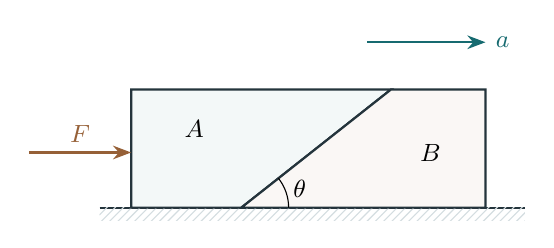
\begin{tikzpicture}

\draw[object] (-.4,0)--(5,0);\fill[pattern=north east lines,pattern color=rulegray] (-.4,-.16) rectangle (5,0);
\filldraw[object,fill=accent!5] (0,0)--(1.4,0)--(3.3,1.5)--(0,1.5)--cycle;
\filldraw[object,fill=warm!5] (1.4,0)--(4.5,0)--(4.5,1.5)--(3.3,1.5)--cycle;
\node at (.8,1) {$A$};\node at (3.8,.7) {$B$};
\draw[force] (-1.3,.7)--(0,.7) node[midway,above] {$F$};
\draw (2,0) arc(0:38.29:.6);\node at (2.14,.24) {$\theta$};\draw[motion] (3,2.1)--(4.5,2.1) node[right] {$a$};

\end{tikzpicture}
\figcaption{图 2.7\quad 接触斜面向右升高；两木块都与地面保持接触。}
\end{minipage}\end{center}

\Needspace{5\baselineskip}

\pdfbookmark[3]{题型定位}{q7-h0}

\subsection*{题型定位}

两块木块沿地面共同加速。斜面压力既提供 $B$ 向右的力，又减小 $A$ 的地面支持力。由这两种作用得到压力的上下端，再换成推力范围。

\Needspace{5\baselineskip}

\pdfbookmark[3]{知识点}{q7-h1}

\subsection*{知识点}

牛顿第二定律、光滑斜面的法向力、滑动摩擦、共同加速度。整体水平方程消去内部斜面力，单体的竖直平衡给各自的支持力。两个地面接触都以支持力非负为条件。


\Needspace{5\baselineskip}

\pdfbookmark[3]{物理图像}{q7-h2}

\subsection*{物理图像}

图2.7 的斜面向右升高。解图2.7A 上，同一对斜面压力对 $B$ 向右下、对 $A$ 向左上。增大压力时，$B$ 得到更大的向右分力，地面摩擦也随支持力增大。同时 $A$ 的地面支持力减小，到零时正要离地。斜面光滑，两块接触面之间只有法向力。

\Needspace{5\baselineskip}

\pdfbookmark[3]{解题入口}{q7-h3}

\subsection*{解题入口}

先隔离 $B$，把地面支持力 $m_Bg+N\cos\theta$ 代进 $N\sin\theta-\mu R_B=m_Ba$。由 $a>0$ 得压力下限，再由 $A$ 的 $R_A=m_Ag-N\cos\theta\geq0$ 得上限。要求两限之间有可取的 $N$，就能求出 $\mu$ 的范围；用整体加速度把压力条件换成 $F$ 的范围。

\Needspace{5\baselineskip}

\pdfbookmark[3]{标准解法}{q7-h4}

\subsection*{标准解法}

两个木块已在地面上向右滑动，解图2.7A 中的两支地面摩擦箭头都指向左方。记共同加速度为 $a>0$，斜面间的法向力大小为 $N$。斜面向右升高，它对 $B$ 的法向力指向右下方，对 $A$ 的法向力指向左上方，竖直分量的大小均为 $N\cos\theta$。
\begin{center}\begin{minipage}{\linewidth}\centering\begin{tikzpicture}

\begin{scope}
\fill (0,0) circle(2pt);\node at (0,2.9) {$A$};
\draw[force] (0,0)--(1.28,0) node[right] {$F$};
\draw[force] (0,0)--(-.16,0);\node[left] at (-.17,0) {$\mu R_A$};
\draw[force] (0,0)--(-.8,.8) node[above left] {$N$};
\draw[force] (0,0)--(0,.8) node[above] {$R_A$};
\draw[force] (0,0)--(0,-1.6) node[below] {$m_Ag$};
\end{scope}
\begin{scope}[xshift=5.6cm]
\fill (0,0) circle(2pt);\node at (0,2.9) {$B$};
\draw[force] (0,0)--(.8,-.8) node[below right] {$N$};
\draw[force] (0,0)--(-.48,0) node[left] {$\mu R_B$};
\draw[force] (0,0)--(0,2.4) node[above] {$R_B$};
\draw[force] (0,0)--(0,-1.6) node[below] {$m_Bg$};
\end{scope}

\end{tikzpicture}
\figcaption{解图 2.7A\quad 图取$m_A=m_B$、$\theta=45^\circ$、$\mu=0.2$及$a=0.2g$。$A$的地面支持力较小，$B$的地面支持力较大。}
\end{minipage}\end{center}
竖直方向无加速度，故两块的地面支持力为
\[
R_A=m_Ag-N\cos\theta,\qquad
R_B=m_Bg+N\cos\theta.
\]
随 $N$ 增加，$A$ 的支持力减少 $N\cos\theta$，$B$ 的支持力增加同样多，地面承担的总力仍为 $R_A+R_B=(m_A+m_B)g$。$B$ 的支持力始终为正，$A$ 保持接触的条件为 $R_A\geq0$，即
\[
N\leq\frac{m_Ag}{\cos\theta}. \tag{1}
\]
对 $B$ 水平方向列式，有
\[
N\sin\theta-\mu(m_Bg+N\cos\theta)=m_Ba>0.
\]
$B$ 的向右净力随 $N$ 的斜率为 $\sin\theta-\mu\cos\theta$，而在 $N=0$ 时其值为 $-\mu m_Bg$。要使净力为正，斜率须为正，因而
\[
N>\frac{\mu m_Bg}{\sin\theta-\mu\cos\theta}. \tag{2}
\]
斜率来自两个分量的差。每增加一单位压力，$B$ 得到 $\sin\theta$ 的向右力，地面摩擦同时增加 $\mu\cos\theta$。

\subsubsection*{压力区间存在的条件}
由 $R_A=0$ 定出的上端须大于由 $a=0$ 定出的下端，因此
\[
\frac{\mu m_Bg}{\sin\theta-\mu\cos\theta}
<\frac{m_Ag}{\cos\theta}.
\]
在正分母条件下交叉相乘，得到
\[
\mu m_B\cos\theta<m_A\sin\theta-\mu m_A\cos\theta,
\quad\boxed{0\leq\mu<\frac{m_A}{m_A+m_B}\tan\theta}.
\]
这个更强的条件已经保证 $\mu<\tan\theta$。

\subsubsection*{由压力换成推力}
整个系统的水平外力为 $F-\mu(R_A+R_B)$，因此
\[
a=\frac{F}{m_A+m_B}-\mu g.
\]
再代入 $B$ 的方程，公共的重力摩擦项抵消，得到
\[
N(\sin\theta-\mu\cos\theta)
=\frac{m_B}{m_A+m_B}F.
\]
于是 (2) 给出 $F>\mu(m_A+m_B)g$，(1) 给出有限上限，合并为
\[
\boxed{\mu(m_A+m_B)g<F
\leq\frac{m_A}{m_B}(m_A+m_B)(\tan\theta-\mu)g}.
\]
$F$ 取下端时 $a=0$，题设取 $a>0$，故范围从开端点开始。$F$ 取上端时 $R_A=0$，题设把这一临界接触状态计入。若另取 $R_A>0$，相应的推力范围在上端也为开区间。

令 $\mu=0$，地面水平摩擦消失，上限仍由 $N\cos\theta=m_Ag$ 决定。此时 $F$ 增大只会使 $N$ 继续增大，恰在这个等式成立时 $A$ 的地面支持力降到零。
\subsubsection*{两块木块的加速度与接触力}
解图2.7A 中，$A$ 的水平力有向右的推力，以及向左的摩擦和斜面压力分量，因此
\[
F-\mu(m_Ag-N\cos\theta)-N\sin\theta=m_Aa.
\]
将 $A,B$ 各自的净力除以相应质量，并令两块的加速度相同，得到
\[
\frac{F-\mu m_Ag-N(\sin\theta-\mu\cos\theta)}{m_A}
=\frac{N(\sin\theta-\mu\cos\theta)-\mu m_Bg}{m_B}.
\]
将质量交叉相乘，重力摩擦项相消，得到
\[
m_BF=(m_A+m_B)N(\sin\theta-\mu\cos\theta).
\]
消元时，两块的地面摩擦各随支持力变化，合计仍为 $\mu(m_A+m_B)g$，所以只留下 $F$ 和接触力。

给定区间内的 $F$，用整体式求得 $a>0$，再由上式求 $N$。由于 $\sin\theta-\mu\cos\theta>0$ 且 $F>0$，接触压力为正。推力上限保证 $R_A\geq0$，而 $R_B=m_Bg+N\cos\theta>0$。这组接触力代入两个单体方程后，两块的竖直加速度均为零，水平方向得到同一个 $a$，正是图2.7A 所画的共同滑动状态。推力达到上限时，$A$ 的地面支持力降到零。超过上限后，需按允许 $A$ 离地的接触条件求运动。


\Needspace{5\baselineskip}

\pdfbookmark[3]{关键洞察}{q7-h5}

\subsection*{关键洞察}

$N$ 的下限由 $B$ 的水平运动给出，上限由 $A$ 的竖直接触给出。两条限制一起决定 $\mu$；整体加速度随后把同一段压力范围换成推力范围。

\Needspace{5\baselineskip}

\pdfbookmark[3]{易错点}{q7-h6}

\subsection*{易错点}

\begin{itemize}
\item 在解图2.7A 中，对 $B$ 的压力竖直分量向下，故 $R_B=m_Bg+N\cos\theta$。对 $A$ 则为 $R_A=m_Ag-N\cos\theta$。
\item 两块都相对地面向右滑动。地面摩擦总量为 $\mu(m_A+m_B)g$。
\item 除以 $\sin\theta-\mu\cos\theta$ 前，先由 $B$ 的正加速度确认它为正。
\end{itemize}

\Needspace{5\baselineskip}

\pdfbookmark[3]{课堂讲解建议}{q7-h7}

\subsection*{课堂讲解建议}

先把解图2.7A 的两支斜面压力同时画长，问两处地面支持力怎样变。$R_A$ 下降，$R_B$ 上升，两者总和等于总重。再问“哪一个端点由 $B$ 决定，哪一个由 $A$ 决定？”$B$ 刚好没有向右净力时是下端，题设排除 $a=0$；$A$ 刚好没有地面支持力时是上端，题设计入 $R_A=0$。最后把 $\mu$ 置零，让学生指出仍给出上限的那支压力分量。

\Needspace{5\baselineskip}

\pdfbookmark[3]{变式训练}{q7-h8}

\subsection*{变式训练}

\begin{enumerate}
\item 地面光滑时推力范围怎样？令 $\mu=0$，两块的水平总方程给 $a=F/(m_A+m_B)$。$B$ 的水平式为 $N\sin\theta=m_Ba$，代入 $R_A=m_Ag-N\cos\theta$ 得
\[
F_{\max}=\frac{m_A(m_A+m_B)}{m_B}g\tan\theta,\qquad
\frac{R_A}{m_Ag}=1-\frac{F}{F_{\max}}.
\]
变图2.7V1 中，红线为 $N\cos\theta/(m_Ag)=F/F_{\max}$，蓝线给剩余支持力。$a>0$ 给 $F>0$，$R_A\geq0$ 给 $F\leq F_{\max}$，当$F=F_{\max}$时，$R_A$降到零。
\begin{center}\begin{minipage}{.98\linewidth}\centering
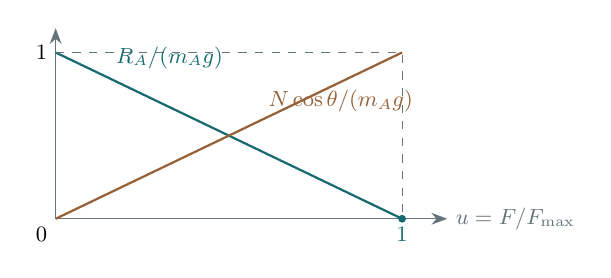
\begin{tikzpicture}[scale=.88,transform shape]
\draw[axis] (0,0)--(5.65,0) node[right] {$u=F/F_{\max}$};
\draw[axis] (0,0)--(0,2.75);
\draw[traj] (0,2.4)--(5,0);
\draw[thick,color=warm] (0,0)--(5,2.4);
\draw[guide] (0,2.4)--(5,2.4)--(5,0);
\node[above right,text=accent] at (.75,2.04) {$R_A/(m_Ag)$};
\node[above right,text=warm] at (2.95,1.416) {$N\cos\theta/(m_Ag)$};
\node[left] at (0,2.4) {$1$};
\node[below left] at (0,0) {$0$};
\fill[accent] (5,0) circle(1.6pt) node[below] {$1$};
\end{tikzpicture}
\figcaption{变图2.7V1\quad 光滑地面上，斜面压力的竖直分量随推力上升，$R_A$ 同时下降。}
\end{minipage}\end{center}
\item 两块质量均为 $m$ 时，摩擦系数和推力满足什么条件？整体方程给 $a=F/(2m)-\mu g$，所以 $F>2\mu mg$。$B$ 的水平式给 $N(\sin\theta-\mu\cos\theta)=F/2$；用 $N\cos\theta\leq mg$ 得 $F\leq2mg(\tan\theta-\mu)$。变图2.7V2 以 $k=\mu/\tan\theta$、$p=F/(2mg\tan\theta)$ 表示两条界线，允许区域为 $k<p\leq1-k$。两线交在 $k=1/2$，故 $\mu<\tfrac12\tan\theta$。
\begin{center}\begin{minipage}{.98\linewidth}\centering
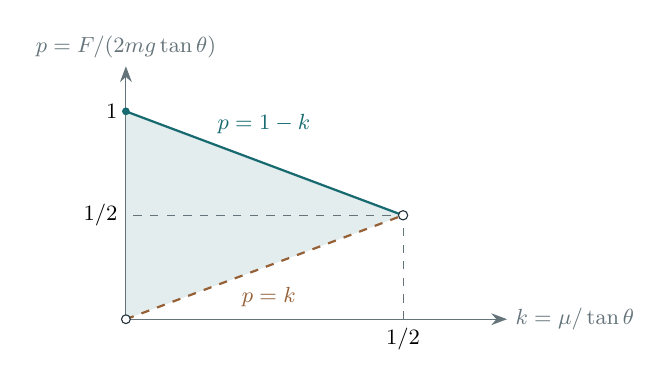
\begin{tikzpicture}[scale=.88,transform shape]
\fill[accent!12] (0,0)--(0,3)--(4,1.5)--cycle;
\draw[axis] (0,0)--(5.5,0) node[right] {$k=\mu/\tan\theta$};
\draw[axis] (0,0)--(0,3.65) node[above] {$p=F/(2mg\tan\theta)$};
\draw[traj] (0,3)--(4,1.5);
\draw[thick,dashed,color=warm] (0,0)--(4,1.5);
\draw[guide] (4,0)--(4,1.5)--(0,1.5);
\node[left] at (0,3) {$1$};
\node[left] at (0,1.5) {$1/2$};
\node[below] at (4,0) {$1/2$};
\node[above right,text=accent] at (1.2,2.55) {$p=1-k$};
\node[below right,text=warm] at (1.55,.58) {$p=k$};
\filldraw[draw=ink,fill=white] (4,1.5) circle(1.9pt);
\filldraw[draw=ink,fill=white] (0,0) circle(1.8pt);
\fill[accent] (0,3) circle(1.6pt);
\end{tikzpicture}
\figcaption{变图2.7V2\quad 两条推力界围成可行区域。下界用虚线表示，交点对应 $a=0$，以空心圆标出。}
\end{minipage}\end{center}
\item 斜接触也粗糙，方程中应加入哪些量？设其静摩擦系数为 $\mu_c$，取变图2.7V3 的右上切向为正，把 $A$ 对 $B$ 的切向力记为 $f_c$。法向力与切向力相加，在 $B$ 上给出水平分量 $H=N\sin\theta+f_c\cos\theta$ 和竖直分量 $Y=-N\cos\theta+f_c\sin\theta$。$A$ 上的两个分量与之相反，因此
\[
R_A=m_Ag+Y,\qquad R_B=m_Bg-Y,\qquad
H+\mu Y=\frac{m_BF}{m_A+m_B}.
\]
最后一式来自 $H-\mu R_B=m_Ba$ 和整体加速度。给定 $F>\mu(m_A+m_B)g$，用这一方程寻找满足 $N\geq0$、$|f_c|\leq\mu_c N$、$R_A,R_B\geq0$ 的 $N,f_c$。图中的摩擦切向分量同时进入水平净力和地面支持力。
\begin{center}\begin{minipage}{.98\linewidth}\centering
\begin{tikzpicture}[scale=.88,transform shape]
\draw[axis] (-2.0,0)--(3.1,0) node[right] {$x$};
\draw[axis] (0,-2.05)--(0,2.0) node[above] {$y$};
\draw[object] (-2.0,-1.50)--(2.3,1.725);
\fill (0,0) circle(1.8pt) node[left,yshift=5pt] {接触点};
\draw[force] (0,0)--(1.26,-1.68) node[right] {$N\hat{\boldsymbol n}$};
\draw[motion] (0,0)--(1.68,1.26) node[above right] {$f_c\hat{\boldsymbol s}\ (f_c>0)$};
\node at (-1.45,.85) {$A$ 侧};
\node at (2.35,-.62) {$B$ 侧};
\end{tikzpicture}
\figcaption{变图2.7V3\quad 图画 $A$ 对 $B$ 的法向力及 $f_c>0$ 时的切向摩擦。}
\end{minipage}\end{center}
\item 推力达到上端时，共同加速度是多少？此时 $N=m_Ag/\cos\theta$，于是 $R_A=0$、$R_B=(m_A+m_B)g$。将这两个量代入 $B$ 的水平方程，得到
\[
a_{\text{上}}=g\left[\frac{m_A}{m_B}\tan\theta-\mu\frac{m_A+m_B}{m_B}\right].
\]
记 $\mu_*=m_A\tan\theta/(m_A+m_B)$、$a_*=g(m_A/m_B)\tan\theta$。变图2.7V4 上是 $a_{\text{上}}/a_*=1-\mu/\mu_*$。在 $\mu/\mu_*=1$ 处加速度降到零，题设取正加速度，所以图上这个端点为空心。
\begin{center}\begin{minipage}{.98\linewidth}\centering
\begin{tikzpicture}[scale=.88,transform shape]
\draw[axis] (0,0)--(5.65,0) node[right] {$\mu/\mu_*$};
\draw[axis] (0,0)--(0,3.05) node[above] {$a_{\text{上}}/a_*$};
\draw[traj] (0,2.65)--(5,0);
\draw[guide] (0,2.65)--(1.1,2.65);
\fill[accent] (0,2.65) circle(1.65pt) node[left] {$1$};
\filldraw[draw=ink,fill=white] (5,0) circle(1.9pt) node[below] {$1$};
\node[below left] at (0,0) {$0$};
\node[above] at (2.8,1.42) {$R_A=0$};
\end{tikzpicture}
\figcaption{变图2.7V4\quad 沿 $A$ 即将离地的一端，$\mu$ 越大，可达到的共同加速度越小。}
\end{minipage}\end{center}
\end{enumerate}

\clearpage

\pdfbookmark[2]{第 8 题 滑块、绳和悬挂重物的相对静止条件}{q8}

\section*{第 8 题\quad 滑块、绳和悬挂重物的相对静止条件}

\tagline{M-02-08}

质量为 $M$ 的滑块 $C$ 位于光滑水平桌面上，滑轮固定在滑块右端。质量均为 $m$ 的物体 $A,B$ 用轻绳连接：$A$ 放在滑块上，绳的这一段水平；$B$ 悬在滑轮外侧。$A$ 与滑块的静摩擦系数为 $\mu$，绳和滑轮质量忽略，转轴光滑。用水平力 $F\geq0$ 向右推动滑块。求使 $A,B$ 与滑块保持相对静止的最小推力。讨论已建立的共同加速状态，悬绳允许倾斜，且 $B$ 不接触滑块。

\begin{center}\begin{minipage}{\linewidth}\centering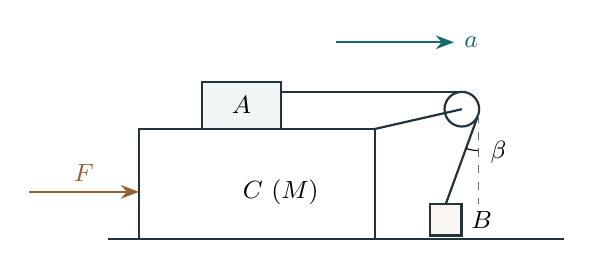
\begin{tikzpicture}

\draw[object] (-.4,0)--(5.4,0);\draw[object] (0,0) rectangle (3,1.4);\node at (1.8,.6) {$C\ (M)$};
\filldraw[object,fill=accent!6] (.8,1.4) rectangle (1.8,2);\node at (1.3,1.7) {$A$};
\draw[object] (4.1,1.65) circle(.22);\draw[object] (3,1.4)--(4.1,1.65);\draw[object] (1.8,1.87)--(4.1,1.87);
\draw[object] (4.3067,1.5748)--(3.8963,.4471);\filldraw[object,fill=warm!6] (3.6963,.0471) rectangle (4.0963,.4471);\node[right] at (4.0963,.2471) {$B$};
\draw[guide] (4.3067,1.5748)--(4.3067,.45);\draw (4.3067,1.1248) arc(270:250:.45);\node[right] at (4.34,1.10) {$\beta$};
\draw[force] (-1.4,.6)--(0,.6) node[midway,above] {$F$};\draw[motion] (2.5,2.5)--(4,2.5) node[right] {$a$};

\end{tikzpicture}
\figcaption{图 2.8\quad 共同向右加速时，悬绳向左倾斜。图中的侧面留有间隙，表示 $B$ 不与滑块接触。}
\end{minipage}\end{center}

\Needspace{5\baselineskip}

\pdfbookmark[3]{题型定位}{q8-h0}

\subsection*{题型定位}

水平加速的滑块上，两个重物通过一根绳保持相对静止。悬物的张力水平分量给出它的加速度，桌上重物所需静摩擦则决定最小推力。

\Needspace{5\baselineskip}

\pdfbookmark[3]{知识点}{q8-h1}

\subsection*{知识点}

地面系中的共同加速度、轻绳通过光滑滑轮时两段张力大小相等、静摩擦范围。改用滑块参考系时，加上水平向左的惯性力，原来的运动方程便写成平衡方程。


\Needspace{5\baselineskip}

\pdfbookmark[3]{物理图像}{q8-h2}

\subsection*{物理图像}

图2.8 的悬绳下端向左偏，因而对 $B$ 的张力指向右上。解图2.8A 中，张力的竖直分量平衡重力，水平分量使 $B$ 向右加速。滑块上的 $A$ 受到整支水平张力，它与所需净力 $ma$ 的差由向左的静摩擦抵消。

\Needspace{5\baselineskip}

\pdfbookmark[3]{解题入口}{q8-h3}

\subsection*{解题入口}

以解图2.8A 的绳倾角 $\beta$ 列式
\[
T\sin\beta=ma,\qquad T\cos\beta=mg,\qquad T-f=ma.
\]
前两式给 $T=m\sqrt{a^2+g^2}$，后一式给所需静摩擦 $f$。将 $f\leq\mu mg$ 与整体方程 $F=(M+2m)a$ 合用，分别求 $\mu=0$、$0<\mu<1$ 和 $\mu\geq1$ 的结果。

\Needspace{5\baselineskip}

\pdfbookmark[3]{标准解法}{q8-h4}

\subsection*{标准解法}

在题设的共同运动状态中，$A,B,C$ 都以同一个水平加速度 $a$ 运动，竖直加速度为零。图2.8 的悬绳下端在滑轮左下方，因此张力在平衡 $B$ 重力的同时，还能给出向右的水平分量。当 $a=0$ 时，绳沿竖直方向。
\begin{center}\begin{minipage}{\linewidth}\centering\begin{tikzpicture}

\begin{scope}
\fill (0,0) circle(2pt);\node at (0,2) {$A$};
\draw[force] (0,0)--(1.3834,0) node[right] {$T$};\draw[force] (0,0)--(-.9102,0) node[left] {$f$};
\draw[force] (0,0)--(0,1.3) node[above] {$N$};\draw[force] (0,0)--(0,-1.3) node[below] {$mg$};
\end{scope}
\begin{scope}[xshift=6cm]
\fill (0,0) circle(2pt);\node at (0,2) {$B$};
\draw[force] (0,0)--(.4732,1.3) node[above right] {$T$};\draw[force] (0,0)--(0,-1.3) node[below] {$mg$};
\draw[guide] (0,0)--(0,1.3);\draw (0,.5) arc(90:70:.5);\node at (.22,.74) {$\beta$};
\draw[motion] (.4,-.5)--(1.6,-.5) node[right] {$a$};
\end{scope}

\end{tikzpicture}
\figcaption{解图 2.8A\quad $B$的张力竖直分量平衡重力，水平分量使它向右加速。$A$的静摩擦向左。}
\end{minipage}\end{center}
解图 2.8A 中绳与竖直的夹角为 $\beta$，张力对 $B$ 朝右上方。由两个分量方程，
\[
T\sin\beta=ma,\qquad T\cos\beta=mg,
\]
因此
\[
\tan\beta=\frac ag,\qquad T=m\sqrt{a^2+g^2}.
\]
$A$ 所在绳段水平，张力向右。规定作用于 $A$ 的摩擦向左时大小为 $f$，则
\[
T-f=ma,\qquad N_A=mg,
\quad f=m(\sqrt{a^2+g^2}-a)>0.
\]
$g>0$ 使 $T>ma$，所以在任何有限 $a$ 下，$A$ 所受静摩擦都指向左方。解图2.8A 中，这支箭头的大小正好补足张力与所需水平净力的差。

\subsubsection*{静摩擦不等式与推力下限}
相对静止要求
\[
\sqrt{a^2+g^2}-a\leq\mu g.
\]
对 $\mu>0$，将 $a$ 移到右侧，得到 $\sqrt{a^2+g^2}\leq a+\mu g$。两边均非负，平方保持不等号方向：
\[
a^2+g^2\leq a^2+2\mu ag+\mu^2g^2,
\qquad a\geq\frac{1-\mu^2}{2\mu}g.
\]
整体水平外力只有 $F$，桌面光滑，故 $F=(M+2m)a$。结合 $a\geq0$，有
\[
\boxed{F_{\min}=\begin{cases}
(M+2m)g(1-\mu^2)/(2\mu),&0<\mu<1,\\
0,&\mu\geq1.
\end{cases}}
\]
$\mu=0$ 时，任何有限 $a$ 下所需摩擦都大于零，因而不存在有限推力使三物体按题设共同运动。$\mu\geq1$ 时，$a=0$ 已能承受 $T=mg$，所以没有正的推力下限。

\subsubsection*{推力增大为何反而更容易维持}
将所需摩擦有理化：
\[
f=\frac{mg^2}{\sqrt{a^2+g^2}+a},\qquad
\frac{\dd f}{\dd a}=m\left(\frac a{\sqrt{a^2+g^2}}-1\right)<0.
\]
随 $a$ 增大，作用在 $A$ 上的水平张力 $T$ 增大，但 $T-ma$ 逐渐趋近于零。只要 $B$ 仍悬空且与滑块无接触，一旦所需摩擦降到 $\mu mg$，继续增大推力留下的摩擦余量更大。在滑块参考系里，$B$ 受到向左的惯性力 $ma$ 和向下的重力 $mg$，解图2.8A 的斜向张力正好平衡这两个分量。

若悬绳最初竖直，从静止突然施加推力时，$B$ 会相对滑块摆动。题中所求的状态对应悬绳处在倾角 $\beta$，且 $B$ 相对滑块的速度为零。
\subsubsection*{滑轮传给滑块的力}
题图2.8中，轻绳在滑轮两侧张力大小相同，方向分别沿水平绳段和斜绳段。
绳对滑轮的水平合力向左，大小为$T+T\sin\beta$，
竖直合力向下，大小为$T\cos\beta=mg$。
这些力通过固定滑轮的支架传给滑块$C$。
解图2.8A中滑块对$A$的摩擦向左，所以$A$对滑块的摩擦向右，大小仍为$f$。
因此滑块自身的水平方程为
\[
F+f-T-T\sin\beta=Ma.
\]
由$T-f=ma$、$T\sin\beta=ma$逐项代入，得
$F-ma-ma=Ma$。两项 $ma$ 分别由桌上物体的张力与摩擦之差、斜绳段的张力水平分量给出，合在一起便是整体方程 $F=(M+2m)a$。竖直方向上，滑块承担自身重量、$A$ 的压力和滑轮传下的 $T\cos\beta=mg$，故桌面对滑块的支持力为 $(M+2m)g$。

在$0<\mu<1$的临界推力处，
\[
a_{\min}=\frac{1-\mu^2}{2\mu}g,\qquad
T_{\min}=\frac{1+\mu^2}{2\mu}mg,\qquad f=\mu mg.
\]
所以最小推力确对应桌上物体的静摩擦恰达上限。
当 $\mu=1$ 时，$a_{\min}=0$ 恰使 $f=\mu mg$。当 $\mu>1$ 时，$a=0$ 已满足 $f=mg<\mu mg$，所以最小推力仍取零。


\Needspace{5\baselineskip}

\pdfbookmark[3]{关键洞察}{q8-h5}

\subsection*{关键洞察}

$B$ 所需的张力由水平分量 $ma$ 和竖直分量 $mg$ 合成。$A$ 获得整支张力，摩擦只需补足 $T-ma$。将这个差有理化，便看出它随 $a$ 增大而减小。

\Needspace{5\baselineskip}

\pdfbookmark[3]{易错点}{q8-h6}

\subsection*{易错点}

\begin{itemize}
\item 对 $B$ 的竖直分量是 $T\cos\beta=mg$。当 $a>0$ 时，张力还含向右分量 $ma$。
\item $A$ 受到的静摩擦向左，因为整支张力大于它的水平净力 $ma$。
\item 当 $\mu\geq1$，$a=0$ 时的 $f=mg$ 已在静摩擦范围内，最小推力取零。
\end{itemize}

\Needspace{5\baselineskip}

\pdfbookmark[3]{课堂讲解建议}{q8-h7}

\subsection*{课堂讲解建议}

先请学生在解图2.8A 上遮住 $B$ 的斜向张力，只保留重力和向右的加速度箭头，再按两个分量把张力画回来。随后问“加速度增大后，$T$ 与 $ma$ 都增大，哪一个增得更快？”由 $f=mg^2/(\sqrt{a^2+g^2}+a)$ 看出它们的差在减小。最后比较突然推滑块和图中的相对静止状态，指出前者的悬绳起初还在摆动。

\Needspace{5\baselineskip}

\pdfbookmark[3]{变式训练}{q8-h8}

\subsection*{变式训练}

\begin{enumerate}
\item $A$ 与滑块无摩擦时，能否用有限推力维持共同运动？由 $B$ 的两个分量得到 $T=m\sqrt{a^2+g^2}$。它也是 $A$ 所受的水平拉力；若只靠这支张力，$A$ 的水平加速度为 $\sqrt{a^2+g^2}>a$，将相对滑块向右运动。令 $q=a/g$，变图2.8V1 上 $f/(mg)=1/(\sqrt{1+q^2}+q)$ 在所有有限 $q$ 处为正。无摩擦时需要 $f=0$，因此有限推力下无共同运动解。
\begin{center}\begin{minipage}{.98\linewidth}\centering
\begin{tikzpicture}[scale=.88,transform shape]
\draw[axis] (0,0)--(6.35,0) node[right] {$q=a/g$};
\draw[axis] (0,0)--(0,3.05) node[above] {$f/(mg)$};
\draw[traj,domain=0:4,samples=100] plot ({1.45*\x},{2.55/(sqrt(1+\x*\x)+\x)});
\draw[guide] (0,2.55)--(.55,2.55);
\fill[accent] (0,2.55) circle(1.6pt) node[left] {$1$};
\node[below left] at (0,0) {$0$};
\node[below] at (2.9,0) {$2$};
\node[below] at (5.8,0) {$4$};
\node[above right,text=accent] at (2.65,.67) {$\sqrt{1+q^2}-q$};
\end{tikzpicture}
\figcaption{变图2.8V1\quad 所需静摩擦随加速度下降，曲线在所有有限 $q$ 处均高于横轴。}
\end{minipage}\end{center}
\item 若两物体质量分别为 $m_A,m_B$，怎样确定推力条件？对 $B$ 分解张力，得 $T=m_B\sqrt{a^2+g^2}$。规定 $A$ 的静摩擦向左为正，得 $f=T-m_Aa$。令 $r=m_B/m_A$、$q=a/g$，则
\[
\phi(q)=\frac{f}{m_Ag}=r\sqrt{1+q^2}-q,\qquad
|\phi(q)|\leq\mu,\qquad F=(M+m_A+m_B)gq.
\]
可由曲线与 $\phi=\pm\mu$ 的交点求端点。取 $c=\pm\mu$，方程 $\phi=c$ 平方后为 $(r^2-1)q^2-2cq+r^2-c^2=0$，并取满足 $q\geq0$、$q+c>0$ 的根。变图2.8V2 取 $r=3/4,\ \mu=1/4$，曲线单调下降，分别在 $q_-=(-4+6\sqrt2)/7$ 和 $q_+=(4+6\sqrt2)/7$ 进入与离开阴影带。零点 $q_0=3/\sqrt7$ 左侧的摩擦向左，右侧向右。判区间时可再考虑端点 $q=0$。若 $0<r<1$，因 $\phi'(q)=rq/\sqrt{1+q^2}-1<0$，曲线从 $\phi(0)=r$ 单调降至负无穷。因而 $\mu\geq r$ 时取 $q_-=0$，否则由 $\phi=\mu$ 取下端；上端总由 $\phi=-\mu$ 给出。若 $r=1$，沿用等质量结果。若 $r>1$，$\phi$ 始终为正，在 $q_*=1/\sqrt{r^2-1}$ 处取最小值 $\sqrt{r^2-1}$。所以 $\mu$ 小于该最小值时无共转区间，等于它时只取 $q_*$，大于它时以 $\phi\leq\mu$ 的两侧为限。$\mu\geq r$ 时下端也可取零。
\begin{center}\begin{minipage}{.98\linewidth}\centering
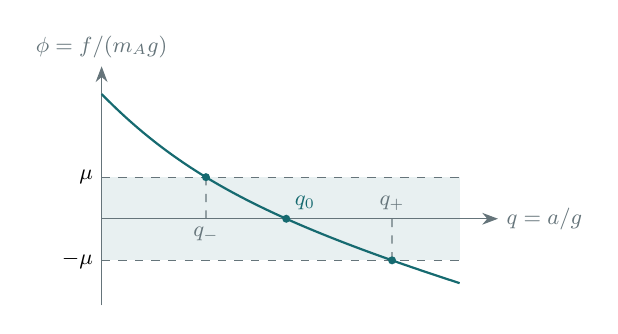
\begin{tikzpicture}[scale=.88,transform shape]
\fill[accent!10] (0,-.6) rectangle (5.17,.6);
\draw[axis] (0,0)--(5.72,0) node[right] {$q=a/g$};
\draw[axis] (0,-1.25)--(0,2.2) node[above] {$\phi=f/(m_Ag)$};
\draw[guide] (0,.6)--(5.17,.6);
\draw[guide] (0,-.6)--(5.17,-.6);
\draw[traj,domain=0:2.2,samples=110] plot ({2.35*\x},{2.4*(.75*sqrt(1+\x*\x)-\x)});
\coordinate (L) at ({2.35*(-4+6*sqrt(2))/7},.6);
\coordinate (U) at ({2.35*(4+6*sqrt(2))/7},-.6);
\coordinate (Z) at ({2.35*3/sqrt(7)},0);
\draw[guide] (L)--({2.35*(-4+6*sqrt(2))/7},0) node[below] {$q_-$};
\draw[guide] (U)--({2.35*(4+6*sqrt(2))/7},0) node[above] {$q_+$};
\fill[accent] (L) circle(1.65pt);\fill[accent] (U) circle(1.65pt);
\fill[accent] (Z) circle(1.65pt) node[above right] {$q_0$};
\node[left] at (0,.6) {$\mu$};
\node[left] at (0,-.6) {$-\mu$};
\end{tikzpicture}
\figcaption{变图2.8V2\quad 取 $m_B/m_A=3/4$、$\mu=1/4$，曲线落在阴影带的部分可以维持共同运动。}
\end{minipage}\end{center}
\item 在滑块参考系中求摩擦力和绳倾角。$B$ 相对滑块静止。把向左的惯性力 $ma$ 和向下的重力 $mg$ 像变图2.8V3 那样首尾相接，闭合向量是张力。因此 $\tan\beta=a/g$，$T=m\sqrt{a^2+g^2}$。对 $A$，向右张力平衡向左的惯性力和静摩擦，给出 $T=ma+f$。于是 $f=m(\sqrt{a^2+g^2}-a)$，它须位于 $0\leq f\leq\mu mg$ 内。变图2.8V3取 $a=g$，两条直角边等长，此时 $\beta=45^\circ$、$f=(\sqrt2-1)mg$。
\begin{center}\begin{minipage}{.98\linewidth}\centering
\begin{tikzpicture}[scale=.88,transform shape]
\coordinate (O) at (0,0);
\coordinate (L) at (-1.65,0);
\coordinate (D) at (-1.65,-1.65);
\draw[force] (O)--(L) node[midway,above] {$ma$};
\draw[force] (L)--(D) node[midway,left] {$mg$};
\draw[motion] (D)--(O) node[midway,below right] {$T$};
\draw[thin] (-1.43,0)--(-1.43,-.22)--(-1.65,-.22);
\fill (O) circle(1.55pt);
\node[above right] at (.45,.05) {$B$，滑块参考系};
\node[right] at (.45,-.6) {$a=g$};
\end{tikzpicture}
\figcaption{变图2.8V3\quad 重力、惯性力和张力首尾相接，三个向量之和为零。}
\end{minipage}\end{center}
\item 取 $\mu=1/2$，求临界加速度、绳倾角和张力。临界时 $f=mg/2$，所以 $\sqrt{a^2+g^2}=a+g/2$。平方并约去 $a^2$，得 $a_{\min}=3g/4$。变图2.8V4 的水平边为 $ma=3mg/4$，竖直边为 $mg$，斜边为 $T=5mg/4$。斜边与竖直线的夹角为 $\beta=\arctan(3/4)\approx36.87^\circ$。由于 $T$ 随 $a\geq0$ 增大而增大，这也是满足静摩擦条件时的最小张力。
\begin{center}\begin{minipage}{.98\linewidth}\centering
\begin{tikzpicture}[scale=.88,transform shape]
\coordinate (O) at (0,0);
\coordinate (X) at (1.8,0);
\coordinate (T) at (1.8,2.4);
\draw[force] (O)--(X) node[midway,below] {$3mg/4$};
\draw[force] (X)--(T) node[midway,right] {$mg$};
\draw[motion] (O)--(T) node[midway,above left] {$5mg/4$};
\draw[guide] (O)--(0,2.55);
\draw[object] (0,.7) arc (90:53.130102:.7);
\node at (.32,.86) {$\beta$};
\draw[thin] (1.6,0)--(1.6,.2)--(1.8,.2);
\end{tikzpicture}
\figcaption{变图2.8V4\quad 临界状态的张力三角形，两直角边之比为 $3:4$。}
\end{minipage}\end{center}
\end{enumerate}

\clearpage

\pdfbookmark[2]{第 9 题 旋转平台沟槽中双球的稳定位置}{q9}

\section*{第 9 题\quad 旋转平台沟槽中双球的稳定位置}

\tagline{M-02-09}

水平平台以角速度 $\omega>0$ 绕中心竖直轴转动。两个径向沟槽内分别放小球 $A,B$，质量为 $m_A,m_B$。$A$ 与槽底的静摩擦系数为 $\mu$，$B$ 所在槽光滑。长为 $\ell$ 的轻绳绕过光滑中心轴，连接两球；轴半径可忽略。求两球可以与平台保持相对静止时，$A$ 到中心的距离 $x$ 的范围。忽略球和轴的尺寸，槽长至少为 $\ell$。

\begin{center}\begin{minipage}{\linewidth}\centering\begin{tikzpicture}

\draw[object] (0,0) circle(2.4);\draw[object] (-2.2,.17)--(2.2,.17);\draw[object] (-2.2,-.17)--(2.2,-.17);
\draw[object] (-1.55,0)--(1.2,0);\filldraw[object,fill=accent!12] (-1.55,0) circle(.15);\filldraw[object,fill=warm!12] (1.2,0) circle(.15);\fill (0,0) circle(2pt);
\node[above] at (-1.55,.2) {$A$（粗糙）};\node[above] at (1.2,.2) {$B$（光滑）};\node[below] at (0,0) {$O$};
\draw[thin,<->] (-1.55,-.6)--(0,-.6) node[midway,below] {$x$};\draw[thin,<->] (0,-.6)--(1.2,-.6) node[midway,below] {$\ell-x$};
\draw[motion] (2.75,-.7) arc(-15:55:2.85);\node[right] at (2.7,.8) {$\omega$};

\end{tikzpicture}
\figcaption{图 2.9\quad 绳长把两个向心运动联系起来，槽沿半径方向。}
\end{minipage}\end{center}

\Needspace{5\baselineskip}

\pdfbookmark[3]{题型定位}{q9-h0}

\subsection*{题型定位}

旋转平台上两个小球沿径向槽共转。绳长把两个半径关联起来，光滑槽中的小球确定张力，粗糙槽中的小球靠静摩擦补足其向心需求。

\Needspace{5\baselineskip}

\pdfbookmark[3]{知识点}{q9-h1}

\subsection*{知识点}

圆周运动、轻绳长度约束、径向槽的支持、静摩擦的大小和方向。由所需静摩擦的范围求可维持的位置，再与绳长允许的半径相交。若要讨论无摩擦位置受扰后的运动，另列两球沿槽的加速度方程。


\Needspace{5\baselineskip}

\pdfbookmark[3]{物理图像}{q9-h2}

\subsection*{物理图像}

图2.9 中 $AO=x$，$BO=\ell-x$。两球各有一支指向 $O$ 的张力。$A$ 向外移动时，$B$ 向内移动，绳张力随 $B$ 的向心需求减小；与此同时，$A$ 的向心需求增大。因此解图2.9A 中以 $x_0$ 为分界，内侧位置需向外摩擦，外侧位置需向内摩擦。

\Needspace{5\baselineskip}

\pdfbookmark[3]{解题入口}{q9-h3}

\subsection*{解题入口}

取小球 $A$ 的静摩擦沿径向向外为正。地面系的两个向心方程为
\[
T-f=m_A\omega^2x,\qquad T=m_B\omega^2(\ell-x).
\]
消去 $T$，先由 $f=0$ 找到 $x_0=m_B\ell/(m_A+m_B)$，再用 $|f|\leq\mu m_Ag$ 求出两侧允许偏移量，最后按 $0\leq x\leq\ell$ 取实际区间。

\Needspace{5\baselineskip}

\pdfbookmark[3]{标准解法}{q9-h4}

\subsection*{标准解法}

设 $A$ 距中心 $x$，绳长约束给出 $B$ 距中心 $\ell-x$。两球位于中心两侧的径向槽中，绳张力均指向中心。槽底支持力平衡重力，$N_A=m_Ag$。共转时两球的加速度都指向转轴，中心处取零。所需向心力由张力和槽底摩擦合成。
\begin{center}\begin{minipage}{\linewidth}\centering\begin{tikzpicture}

\begin{scope}
\draw[guide] (-2,0)--(2,0);\fill (0,0) circle(2pt);\node[above] at (0,.6) {$A$};
\draw[force] (0,0)--(1.7,0) node[right] {$T$，向心};\draw[force] (0,0)--(-1.4,0) node[left] {$f>0$，向外};
\node[align=center] at (0,-1.1) {$x<x_0:\ f>0$\\$x>x_0:\ f<0$};
\end{scope}
\begin{scope}[xshift=6.4cm]
\draw[axis] (-.2,0)--(4,0) node[right] {$x$};\draw[traj,line width=2pt] (.9,0)--(2.7,0);
\draw[guide] (1.8,-.5)--(1.8,.6);\node[above] at (1.8,.6) {$x_0$};
\node[below] at (.9,-.05) {$x_0-\Delta x$};\node[below] at (2.7,-.05) {$x_0+\Delta x$};
\node[above] at (0,0) {$0$};\node[above] at (3.6,0) {$\ell$};
\end{scope}

\end{tikzpicture}
\figcaption{解图 2.9A\quad 摩擦可向内也可向外；代数区间还要与几何区间相交。}
\end{minipage}\end{center}
先看光滑槽中的 $B$，向心力仅由张力提供：
\[
T=m_B\omega^2(\ell-x).
\]
对 $A$ 规定静摩擦向外为正，地面系径向方程为
\[
-T+f=-m_A\omega^2x.
\]
消去 $T$，得到
\[
f=\omega^2\{m_B\ell-(m_A+m_B)x\}.
\]
无须摩擦的位置为
\[
x_0=\frac{m_B\ell}{m_A+m_B}.
\]
解图2.9A 规定左侧小球 $A$ 向外为正。$x<x_0$ 时，内向张力超过所需向心力，摩擦沿图示向外。$x>x_0$ 时，张力偏小，摩擦改向中心。

静摩擦限制给出
\[
\omega^2(m_A+m_B)|x-x_0|\leq\mu m_Ag,
\quad |x-x_0|\leq\Delta x,
\quad \Delta x=\frac{\mu m_Ag}{(m_A+m_B)\omega^2}.
\]
再与实际绳长允许的 $0\leq x\leq\ell$ 取交集，故
\[
\boxed{x_{\min}\leq x\leq x_{\max}},\qquad
x_{\min}=\max(0,x_0-\Delta x),\quad
x_{\max}=\min(\ell,x_0+\Delta x).
\]
当 $\omega^2>\mu m_Ag/(m_B\ell)$ 时，左端 $x_0-\Delta x$ 对应的最小半径大于零；等号时左端恰为零。类似地，$\omega^2>\mu g/\ell$ 使右端 $x_0+\Delta x$ 小于 $\ell$，等号时右端正好为 $\ell$。角速度达到两项阈值中较大的一项时，整段宽度为 $2\Delta x$。在较低转速下，伸出 $[0,\ell]$ 的部分由几何范围截去。

\subsubsection*{端点及无摩擦时的径向扰动}
$x=\ell$ 时，$B$ 位于中心，由它的向心方程得到 $T=0$，这是题设点状轴的极限位置。若要求 $B$ 位于中心之外且绳有正张力，取 $x<\ell$。$\mu=0$ 时只剩 $x_0$。判断这个位置受扰后怎样运动，需要让两球沿槽移动。

当两槽都光滑，绳长给出 $x_B=\ell-x$，相应的两球径向加速度符号相反。消去两球沿槽方程中的共同张力，得到
\[
\ddot x=\omega^2(x-x_0).
\]
偏离会被放大，$x_0$ 是不稳定平衡。有静摩擦时得到的区间是可保持共转的位置集合；转速提高使该集合缩窄，是所需摩擦对位置更敏感的结果。
\subsubsection*{把两侧摩擦限制分别展开}
解图2.9A规定$f>0$向外。$x<x_0$时，张力大于$A$所需向心力，
向外的摩擦抵消多余的内向拉力。它的最大值给出
\[
\omega^2[m_B\ell-(m_A+m_B)x]\leq\mu m_Ag
\quad\Longrightarrow\quad x\geq x_0-\Delta x.
\]
$x>x_0$时张力不足，需要向内摩擦补充，因$f<0$，限制应是
\[
\omega^2[m_B\ell-(m_A+m_B)x]\geq-\mu m_Ag
\quad\Longrightarrow\quad x\leq x_0+\Delta x.
\]
向外摩擦达到上限时对应 $x_0-\Delta x$，向内摩擦达到上限时对应 $x_0+\Delta x$。若摩擦不等式的某个端点超出 $[0,\ell]$，允许位置到沟槽的几何端点为止。

写出无摩擦时两球各自向外为正的沿槽方程，绳长使第二式的加速度为 $-\ddot x$：
\[
m_A\ddot x=m_A\omega^2x-T,\qquad
-m_B\ddot x=m_B\omega^2(\ell-x)-T.
\]
消去$T$后，
$(m_A+m_B)\ddot x=\omega^2[(m_A+m_B)x-m_B\ell]$。
令$\xi=x-x_0$，则$\ddot\xi=\omega^2\xi$，
含随时间增长的$e^{\omega t}$分量，因而唯一的无摩擦平衡不稳定。
径向运动产生的科里奥利力由槽侧壁的横向约束承担，不改变这两个径向方程。
若初始偏移为$\xi_0$、径向相对速度为$u_0$，
则$\xi(t)=\xi_0\cosh\omega t+(u_0/\omega)\sinh\omega t$；
增长项的系数为 $(\xi_0+u_0/\omega)/2$，一般初态下这个系数非零。例如令 $u_0=0$，初始偏移就会按 $\cosh\omega t$ 增大。


\Needspace{5\baselineskip}

\pdfbookmark[3]{关键洞察}{q9-h5}

\subsection*{关键洞察}

$x_0$ 由两球的向心需求相等确定。静摩擦把一个位置扩为一段可以保持的位置，未被截短时半宽正比于 $\mu/\omega^2$。受扰动后是否返回，则由允许径向运动时的方程决定。

\Needspace{5\baselineskip}

\pdfbookmark[3]{易错点}{q9-h6}

\subsection*{易错点}

\begin{itemize}
\item 两段绳长分别为 $x$ 和 $\ell-x$。
\item 竖直支持力为 $m_Ag$；向心加速度位于水平面内。
\item 取向外为正时，$x<x_0$ 给 $f>0$，$x>x_0$ 给 $f<0$，两侧均与 $\mu m_Ag$ 比较。
\item 把允许的代数位置与 $0\leq x\leq\ell$ 相交，才得到小球的实际位置。
\end{itemize}

\Needspace{5\baselineskip}

\pdfbookmark[3]{课堂讲解建议}{q9-h7}

\subsection*{课堂讲解建议}

先让学生在图2.9 上把 $A$ 向外挪一点，同时把 $B$ 向内挪同样的距离，问两球的向心需求怎样改变。由 $B$ 知张力减小，由 $A$ 知需要更大的向心力，所以 $A$ 的摩擦指向中心。再取 $\mu=0$，问把 $A$ 从 $x_0$ 向外挪一点后松手会怎样。由 $\ddot x=\omega^2(x-x_0)>0$ 得它继续向外。最后在图上把 $B$ 移到 $O$，请学生读出此时的张力为零。

\Needspace{5\baselineskip}

\pdfbookmark[3]{变式训练}{q9-h8}

\subsection*{变式训练}

\begin{enumerate}
\item 两槽都光滑，两球的半径各是多少？两球都只有张力提供向心力。由 $T=m_A\omega^2x=m_B\omega^2(\ell-x)$，得
\[
x=\frac{m_B}{m_A+m_B}\ell,\qquad \ell-x=\frac{m_A}{m_A+m_B}\ell.
\]
变图2.9V1 取 $m_A=2m_B$，所以半径分别为 $\ell/3$ 和 $2\ell/3$。尽管右侧的向心加速度是左侧的两倍，它的质量只有左侧的一半，所需张力相同。
\begin{center}\begin{minipage}{.98\linewidth}\centering
\begin{tikzpicture}[scale=.88,transform shape]
\draw[object] (-2.1,0)--(3.7,0);
\filldraw[object,fill=accent!12] (-1.6,0) circle(.14) node[above=3pt] {$A$};
\filldraw[object,fill=warm!12] (3.2,0) circle(.14) node[above=3pt] {$B$};
\fill (0,0) circle(1.5pt) node[above] {$O$};
\draw[force] (-1.6,0)--(-.55,0) node[midway,below=2pt] {$T$};
\draw[force] (3.2,0)--(2.15,0) node[midway,below=2pt] {$T$};
\draw[thin,<->] (-1.6,-.8)--(0,-.8) node[midway,below] {$\ell/3$};
\draw[thin,<->] (0,-.8)--(3.2,-.8) node[midway,below] {$2\ell/3$};
\end{tikzpicture}
\figcaption{变图2.9V1\quad 取 $m_A=2m_B$，质量较大的球在较小半径处，两支张力等大。}
\end{minipage}\end{center}
\item 转速加倍，位置区间的宽度怎样变？由 $\Delta x=\mu m_Ag/[(m_A+m_B)\omega^2]$ 可知，半宽变为 $\Delta x/4$，中心 $x_0$ 保持不变。若两次区间都落在 $[0,\ell]$ 内，实际宽度也变为原来的四分之一。变图2.9V2 取 $x_0=\ell/3$、初始 $\Delta x=\ell/2$。初始代数左端是 $-\ell/6$，实际区间为 $[0,5\ell/6]$；转速加倍后半宽为 $\ell/8$，区间变为 $[5\ell/24,11\ell/24]$。这两段宽度之比是 $3/10$。
\begin{center}\begin{minipage}{.98\linewidth}\centering
\begin{tikzpicture}[scale=.88,transform shape]
\draw[axis] (0,0)--(6.5,0) node[right] {$x/\ell$};
\draw[guide] (0,0)--(0,2.45);
\draw[guide] (6,0)--(6,2.45);
\draw[guide] (2,0)--(2,2.47) node[above] {$x_0/\ell=1/3$};
\draw[traj,line width=1.5pt] (0,1.95)--(5,1.95);
\draw[guide] (-1,1.95)--(0,1.95);
\fill[accent] (0,1.95) circle(1.6pt);
\fill[accent] (5,1.95) circle(1.6pt) node[above] {$5/6$};
\node[above left] at (0,1.95) {$\omega$};
\draw[thick,line width=1.5pt,color=warm] (1.25,.83)--(2.75,.83);
\fill[warm] (1.25,.83) circle(1.6pt) node[below] {$5/24$};
\fill[warm] (2.75,.83) circle(1.6pt) node[below] {$11/24$};
\node[left] at (0,.83) {$2\omega$};
\node[below] at (0,0) {$0$};
\node[below] at (6,0) {$1$};
\end{tikzpicture}
\figcaption{变图2.9V2\quad 上方的左端被中心截住；转速加倍后，两端都在几何范围内。}
\end{minipage}\end{center}
\item 若两槽都粗糙，静摩擦系数分别为 $\mu_A,\mu_B$，位置条件怎样写？两球各自规定向外摩擦为正。记 $P=m_A\omega^2x$、$Q=m_B\omega^2(\ell-x)$，向心方程给 $f_A=T-P$、$f_B=T-Q$。故
\[
T\in[P-\mu_Am_Ag,P+\mu_Am_Ag],\quad
T\in[Q-\mu_Bm_Bg,Q+\mu_Bm_Bg],\quad T\geq0.
\]
变图2.9V3 取一组力的单位 $F_s>0$，令 $P=2F_s$、$Q=3.5F_s$，两球的摩擦限值分别为 $F_s$ 和 $0.75F_s$。阴影中的每个 $T$ 都使两球的静摩擦同时满足条件。在 $0\leq x\leq\ell$ 内，两个区间上端均非负，故两段只要相交，就有非负公共张力。于是位置条件可写成
\[
|P-Q|\leq(\mu_A m_A+\mu_Bm_B)g,
\qquad
|x-x_0|\leq \frac{(\mu_A m_A+\mu_Bm_B)g}{(m_A+m_B)\omega^2}.
\]
最后再取 $0\leq x\leq\ell$。
\begin{center}\begin{minipage}{.98\linewidth}\centering
\begin{tikzpicture}[scale=.88,transform shape]
\fill[accent!12] (4.125,.18) rectangle (4.5,2.12);
\draw[axis] (0,0)--(7,0) node[right] {$T/F_s$};
\draw[traj,line width=1.35pt] (1.5,1.78)--(4.5,1.78);
\draw[thick,line width=1.35pt,color=warm] (4.125,.83)--(6.375,.83);
\foreach \x/\lab in {1.5/1,4.5/3}{\fill[accent] (\x,1.78) circle(1.6pt) node[above] {$\lab$};}
\foreach \x/\lab in {4.125/2.75,6.375/4.25}{\fill[warm] (\x,.83) circle(1.6pt) node[below] {$\lab$};}
\fill[accent] (3,1.78) circle(1.3pt) node[above] {$P/F_s$};
\fill[warm] (5.25,.83) circle(1.3pt) node[above] {$Q/F_s$};
\node[left,text=accent] at (1.5,1.78) {$A$};
\node[left,text=warm] at (4.125,.83) {$B$};
\node[below] at (0,0) {$0$};
\end{tikzpicture}
\figcaption{变图2.9V3\quad 两段允许张力的公共部分为 $2.75F_s\leq T\leq3F_s$。}
\end{minipage}\end{center}
\item 固定位置 $x$，求允许的最大角速度。由 $|f|=(m_A+m_B)\omega^2|x-x_0|$，令它等于 $\mu m_Ag$，得
\[
\omega_{\max}=\sqrt{\frac{\mu m_Ag}{(m_A+m_B)|x-x_0|}}\qquad(x\ne x_0,\ \mu>0).
\]
令 $u=x/\ell$、$u_0=x_0/\ell$、$\omega_s=\sqrt{\mu m_Ag/[(m_A+m_B)\ell]}$。变图2.9V4 取 $u_0=1/3$，画出 $\omega_{\max}/\omega_s=1/\sqrt{|u-u_0|}$。图中两点 $u=1/4,5/12$ 到 $u_0$ 的距离都是 $1/12$，故两者的最大角速度都是 $\sqrt{12}\omega_s$，摩擦方向却相反。在 $x=x_0$，静摩擦为零，所有 $\omega>0$ 均可。若 $\mu=0$，则只有 $x=x_0$ 允许正转速。
\begin{center}\begin{minipage}{.98\linewidth}\centering
\begin{tikzpicture}[scale=.88,transform shape]
\draw[axis] (0,0)--(6.55,0) node[right] {$u=x/\ell$};
\draw[axis] (0,0)--(0,4.18) node[above] {$\omega_{\max}/\omega_s$};
\draw[guide] (2,0)--(2,3.92);
\draw[traj,domain=0:.290,samples=75] plot ({6*\x},{.78/sqrt(1/3-\x)});
\draw[traj,domain=.3766667:1,samples=90] plot ({6*\x},{.78/sqrt(\x-1/3)});
\draw[guide] (1.5,0)--(1.5,{.78*sqrt(12)});
\draw[guide] (2.5,0)--(2.5,{.78*sqrt(12)});
\fill[accent] (1.5,{.78*sqrt(12)}) circle(1.5pt);
\fill[accent] (2.5,{.78*sqrt(12)}) circle(1.5pt);
\node[below] at (1.5,0) {$1/4$};
\node[above] at (2,.03) {$1/3$};
\node[below] at (2.5,0) {$5/12$};
\node[below] at (6,0) {$1$};
\node[above right] at (2.6,3.4) {$u_0=1/3$};
\end{tikzpicture}
\figcaption{变图2.9V4\quad 离 $x_0$ 等远的两个位置有相同的最大角速度。}
\end{minipage}\end{center}
\end{enumerate}

\clearpage

\pdfbookmark[2]{第 10 题 平方阻力竖直上抛的高度与返回速度}{q10}

\section*{第 10 题\quad 平方阻力竖直上抛的高度与返回速度}

\tagline{M-02-10}

质量 $m$ 的物体从地面以速率 $v_0$ 竖直上抛。空气阻力大小为 $\mu v^2$，方向与速度相反，$\mu>0$ 为常数，重力加速度为 $g$。求最大高度，并证明返回地面时的速率为 $v_0\sqrt{mg/(mg+\mu v_0^2)}$。

\begin{center}\begin{minipage}{\linewidth}\centering\begin{tikzpicture}

\draw[object] (-.7,0)--(4.5,0);\draw[axis] (-.3,0)--(-.3,3.5) node[above] {$y$};
\draw[motion] (.7,.2)--(.7,2.9) node[midway,left] {上升};\draw[motion] (2.8,2.9)--(2.8,.2) node[midway,right] {下降};
\draw[guide] (.3,3.1)--(3.3,3.1);\node[right] at (3.3,3.1) {$H$};\node[below] at (.7,0) {$v_0$};\node[below] at (2.8,0) {$u_f$};

\end{tikzpicture}
\figcaption{图 2.10\quad 最高点前后阻力反向，需分别列方程。}
\end{minipage}\end{center}

\Needspace{5\baselineskip}

\pdfbookmark[3]{题型定位}{q10-h0}

\subsection*{题型定位}

平方阻力下的竖直上抛。按最高点分成上升和下降，用速率与位置的微分关系求最大高度及返回速率。

\Needspace{5\baselineskip}

\pdfbookmark[3]{知识点}{q10-h1}

\subsection*{知识点}

阻力方向与有符号速度相反。上升用 $\dot v=v\dd v/\dd y$，下降用 $\dot u=u\dd u/\dd s$。两个积分都在最高点以零速率衔接，下降方程的零加速度给出终端速率。


\Needspace{5\baselineskip}

\pdfbookmark[3]{物理图像}{q10-h2}

\subsection*{物理图像}

解图2.10A 左图中，物体上升，重力与阻力均向下；右图中，物体下降，阻力向上，重力向下。物体从最高点静止下落，向下速率逐渐增长，阻力也增大，使向下加速度逐渐减小。往返机械能的差等于沿路耗散的能量。

\Needspace{5\baselineskip}

\pdfbookmark[3]{解题入口}{q10-h3}

\subsection*{解题入口}

取 $y$ 向上、$s=H-y$ 向下。把上升与下降的力图分别写成 $m\dot v=-mg-\mu v^2$ 与 $m\dot u=mg-\mu u^2$，用链式法则变成位置方程。先积分求 $H$，再把 $s=H$ 代入下降式，用 $e^{-2\mu H/m}$ 消去高度。

\Needspace{5\baselineskip}

\pdfbookmark[3]{标准解法}{q10-h4}

\subsection*{标准解法}

向上为位置坐标 $y$ 的正向。阻力反向于瞬时速度，上升时与重力同向，下降时与重力反向。解图2.10A 的上升图中阻力箭头向下，下降图中阻力箭头向上。用向上的速度写成一个式子时，阻力是 $-\mu|\dot y|\dot y$；下文分别用两个阶段的正速率计算。
\begin{center}\begin{minipage}{\linewidth}\centering\begin{tikzpicture}

\begin{scope}
\fill (0,0) circle(2pt);\node at (0,1.8) {上升};\draw[motion] (-.8,-.4)--(-.8,1) node[above] {$v$};
\draw[force] (-.55,0)--(-.55,-1.2) node[below] {$mg$};\draw[force] (.55,0)--(.55,-.9) node[below] {$\mu v^2$};
\end{scope}
\begin{scope}[xshift=5.3cm]
\fill (0,0) circle(2pt);\node at (0,1.8) {下降};\draw[motion] (-.8,.4)--(-.8,-1) node[below] {$u$};
\draw[force] (0,0)--(0,-1.2) node[below] {$mg$};\draw[force] (0,0)--(0,1.1) node[above] {$\mu u^2$};
\end{scope}

\end{tikzpicture}
\figcaption{解图 2.10A\quad 两个速率 $v,u$ 均取正值；下降的位移 $s$ 从最高点向下量。}
\end{minipage}\end{center}
\subsubsection*{上升段的速度与高度}
上升速率 $v=\dot y>0$，运动方程为 $m\dot v=-mg-\mu v^2$。因题目求高度，使用链式法则 $\dot v=v\,\dd v/\dd y$：
\[
\frac{mv\,\dd v}{mg+\mu v^2}=-\dd y.
\]
从 $(y,v)=(0,v_0)$ 积到 $(y,v)$，有
\[
\frac m{2\mu}\ln\frac{mg+\mu v^2}{mg+\mu v_0^2}=-y,
\quad y=\frac m{2\mu}\ln\frac{mg+\mu v_0^2}{mg+\mu v^2}.
\]
到最高点 $v=0$，故
\[
\boxed{H=\frac m{2\mu}\ln\left(1+\frac{\mu v_0^2}{mg}\right)}.
\]
令 $q=\mu v_0^2/(mg)>0$，有 $\ln(1+q)=\int_0^q(1+z)^{-1}\dd z<q$。所以 $H<v_0^2/(2g)$，阻力使物体在比真空情形更低的位置停升。

\subsubsection*{下降段与返回速率}
从最高点向下量位移 $s=H-y$，下降速率为 $u=\dot s=-\dot y\geq0$。此时
\[
m\dot u=mg-\mu u^2,\qquad
\frac{mu\,\dd u}{mg-\mu u^2}=\dd s.
\]
以 $s=0,u=0$ 为起点积分，得到
\[
s=\frac m{2\mu}\ln\frac{mg}{mg-\mu u^2},
\quad u^2(s)=\frac{mg}{\mu}(1-e^{-2\mu s/m}).
\]
下降方程在 $u=\sqrt{mg/\mu}$ 处的加速度为零。指数式给出 $u^2/(mg/\mu)=1-e^{-2\mu s/m}$，有限 $s$ 时该比值小于1，故积分中的分母为正。继续下落时，速率逐渐趋向终端值 $\sqrt{mg/\mu}$。返回地面时 $s=H$，而上升段结果给出
\[
e^{-2\mu H/m}=\frac{mg}{mg+\mu v_0^2}.
\]
因此
\[
u_f^2=\frac{mg}{\mu}\left(1-\frac{mg}{mg+\mu v_0^2}\right)
=\frac{mgv_0^2}{mg+\mu v_0^2},
\quad\boxed{u_f=v_0\sqrt{\frac{mg}{mg+\mu v_0^2}}}.
\]
若问向上为正的\emph{速度}，答案为 $-u_f$。

\subsubsection*{能量与小阻力极限}
完整往返的机械能损失为 $m(v_0^2-u_f^2)/2>0$。上升和下降各走过距离$H$。取$v_t=\sqrt{mg/\mu}$、$q=v_0^2/v_t^2$，将两段速率平方写到同一个高度坐标上。由上升积分得$v^2/v_t^2=(1+q)^{1-y/H}-1$，下降式给$u^2/v_t^2=1-(1+q)^{y/H-1}$。解图2.10B取$q=3$。沿上升曲线从地面读到$P$，再沿下降曲线从$P$返回地面，可以看见同一高度的两段速率一般不同。

\begin{center}\begin{minipage}{.98\linewidth}\centering
\begin{tikzpicture}
\draw[axis] (0,0)--(6.8,0) node[right] {$y/H$};
\draw[axis] (0,0)--(0,3.1) node[above] {速率平方比};
\draw[traj,domain=0:1,samples=80] plot({6*\x},{.85*(4*exp(-ln(4)*\x)-1)});
\draw[thick,dashed,warm,domain=0:1,samples=80] plot({6*\x},{.85*(1-exp(ln(4)*(\x-1)))});
\fill[accent] (0,2.55) circle(1.55pt) node[left] {$3$};
\fill[warm] (0,.6375) circle(1.55pt) node[left] {$3/4$};
\fill (6,0) circle(1.55pt) node[above right] {$P$};
\node[below] at (6,0) {$1$};\node[below left] at (0,0) {$0$};
\node[above right,accent] at (.9,1.98) {上升 $v^2/v_t^2$};
\node[below right,warm] at (1.1,.43) {下降 $u^2/v_t^2$};
\end{tikzpicture}
\figcaption{解图2.10B\quad 同一高度坐标上的上升与下降速率平方。$P$为最高点。}
\end{minipage}\end{center}

图中两条曲线下的面积相加，乘 $\mu H v_t^2$ 后给阻力耗散。取 $z=y/H$，两条曲线的常数项相消，面积之和为
\[
\int_0^1\!\big[(1+q)^{1-z}-(1+q)^{z-1}\big]\,\dd z
=\frac{(1+q)+(1+q)^{-1}-2}{\ln(1+q)}
=\frac{q^2}{(1+q)\ln(1+q)}.
\]
由于 $\mu H=(m/2)\ln(1+q)$，耗散能量为 $(m/2)v_t^2q^2/(1+q)$，正好等于上、下经过地面时的动能差。
当 $\mu\to0$，用 $\ln(1+q)=q-q^2/2+\cdots$，有
\[
H=\frac{v_0^2}{2g}-\frac{\mu v_0^4}{4mg^2}+O(\mu^2),
\qquad u_f=v_0\left(1-\frac{\mu v_0^2}{2mg}+O(\mu^2)\right).
\]
当$\mu\to0$，高度趋于真空高度$v_0^2/(2g)$，返回速率趋于初速。两式中的一阶修正均为负。
\subsubsection*{始终用向上坐标计算下降段}
若不另设向下位移，可继续用$y$和有符号竖直速度$w_y=\dot y<0$。
解图2.10A的下降力图此时给出
\[
mw_y\frac{\dd w_y}{\dd y}=-mg+\mu w_y^2.
\]
从最高点$(H,0)$积分到$(y,w_y)$，应使用
\[
y-H=\int_0^{w_y}\frac{mq\,\dd q}{-mg+\mu q^2}
=\frac m{2\mu}\ln\frac{mg-\mu w_y^2}{mg}.
\]
在有限下降路程内$|w_y|<\sqrt{mg/\mu}$，对数中的比值为正且不大于一，
因此右边非正，与$y\leq H$一致。
积分原函数含 $\ln|-mg+\mu w_y^2|$。取上下限之差后，绝对值化为 $mg-\mu w_y^2$，与最高点处的 $mg$ 组成无量纲比值。
代入$y=0$、$w_y=-u_f$后，
\[
\left(1-\frac{\mu u_f^2}{mg}\right)
\left(1+\frac{\mu v_0^2}{mg}\right)=1,
\]
仍得到同一返回速率。在向上坐标中，下降的速度和位移增量均为负。改用向下距离后，两者同时变号，积分仍沿解图2.10A 中的同一段下降轨迹。


\Needspace{5\baselineskip}

\pdfbookmark[3]{关键洞察}{q10-h5}

\subsection*{关键洞察}

最高点把两段运动连起来。上升时重力和阻力共同使速率减小，下降时阻力削弱重力的加速作用。返回地面时 $u_f<v_0$，且仍低于终端速率。

\Needspace{5\baselineskip}

\pdfbookmark[3]{易错点}{q10-h6}

\subsection*{易错点}

\begin{itemize}
\item 上升和下降使用各自的正速率，力的方向按图2.10A 确定。
\item 使用有符号速度时，阻力写成 $-\mu|\dot y|\dot y$，实对数由正的端点比值构成。
\item $v_0^2/(2g)$ 是无阻力高度；有限 $\mu$ 时，$\ln(1+q)<q$ 使最大高度更小。
\item 若给返回速度的有符号分量，向上为正时应写 $-u_f$。
\end{itemize}

\Needspace{5\baselineskip}

\pdfbookmark[3]{课堂讲解建议}{q10-h7}

\subsection*{课堂讲解建议}

先让学生在解图2.10A 中画同一个物体在上升、下降时的速度和两个力。问“哪一个力会换向”，答为阻力，因为速度反向。再问“两个阶段路程同为 $H$，怎样比较阻力功”，答为分别积分各段的速率平方。用变图2.10V2 让学生指出下降曲线和终端速率的水平线，读出有限下降的速率始终在水平线下。最后令 $\mu\to0$，由对数的首项得到真空高度。

\Needspace{5\baselineskip}

\pdfbookmark[3]{变式训练}{q10-h8}

\subsection*{变式训练}

\begin{enumerate}
\item 求平方阻力上抛高度的无阻力极限。令 $q=\mu v_0^2/(mg)$，则 $H/(v_0^2/2g)=\ln(1+q)/q$。对小 $q$ 展开 $\ln(1+q)=q-q^2/2+O(q^3)$，故这个比值等于 $1-q/2+O(q^2)$。变图2.10V1 左端趋于1，对应 $H\to v_0^2/(2g)$；当 $q=1$，高度降到真空高度的 $\ln2$ 倍。
\begin{center}\begin{minipage}{.98\linewidth}\centering
\begin{tikzpicture}[scale=0.85,transform shape]
\draw[axis] (0,0)--(6.55,0) node[right] {$q$};
\draw[axis] (0,0)--(0,3.8) node[above] {$H/(v_0^2/2g)$};
\draw[traj,domain=.008:4,samples=100] plot ({1.5*\x},{3.2*ln(1+\x)/\x});
\fill (0,3.2) circle (1.6pt) node[above right] {$q\to0,\ 1$};
\draw[guide] (1.5,0)--(1.5,{3.2*ln(2)})--(0,{3.2*ln(2)});
\node[below] at (1.5,0) {$1$};\node[left] at (0,{3.2*ln(2)}) {$\ln 2$};
\end{tikzpicture}
\figcaption{变图2.10V1\quad 弱阻力极限由曲线左端读出。}
\end{minipage}\end{center}
\item 求下降至高度 $y$ 时的速率。设 $s=H-y$、$v_t=\sqrt{mg/\mu}$。从 $s=0,u=0$ 积分 $u\dd u/[g(1-u^2/v_t^2)]=\dd s$，得到
\[
u(y)=v_t\sqrt{1-e^{-2\mu(H-y)/m}},\qquad 0\leq y\leq H.
\]
变图2.10V2 取 $v_0^2/v_t^2=3$，地面处 $2\mu s/m=\ln4$，图中 $G$ 的纵坐标为 $u_f/v_t=\sqrt3/2$。从最高点到 $G$，曲线不断上升并逐渐变缓。
\begin{center}\begin{minipage}{.98\linewidth}\centering
\begin{tikzpicture}[scale=0.85,transform shape]
\draw[axis] (0,0)--(6.6,0) node[right] {$2\mu s/m$};
\draw[axis] (0,0)--(0,3.62) node[above] {$u/v_t$};
\draw[guide] (0,3)--(6.1,3) node[right] {$1$};
\draw[traj,domain=0:1.38629436,samples=85] plot ({1.5*\x},{3*sqrt(1-exp(-\x))});
\draw[traj,dashed,domain=1.38629436:4,samples=70] plot ({1.5*\x},{3*sqrt(1-exp(-\x))});
\coordinate (G) at ({1.5*ln(4)},{1.5*sqrt(3)});
\draw[guide] ({1.5*ln(4)},0)--(G);\fill (G) circle (1.6pt) node[below right] {$G$};
\node[below] at ({1.5*ln(4)},0) {$\ln4$};
\end{tikzpicture}
\figcaption{变图2.10V2\quad 取 $v_0^2/v_t^2=3$。实线止于地面 $G$，虚线画出继续下落时趋向终端速率的曲线。}
\end{minipage}\end{center}
\item 把阻力改为线性 $kv$，求最大高度。令 $\beta=k/m$，上升方程为 $\dot v+\beta v=-g$。用 $v(0)=v_0$ 得 $v(t)=(v_0+g/\beta)e^{-\beta t}-g/\beta$。置 $v(t_a)=0$，有 $t_a=\beta^{-1}\ln(1+\beta v_0/g)$。积分得
\[
H=\frac{v_0+g/\beta}{\beta}(1-e^{-\beta t_a})-\frac g\beta t_a
=\frac{v_0}{\beta}-\frac g{\beta^2}\ln(1+\beta v_0/g).
\]
变图2.10V3 取 $\beta v_0/g=1$，阴影面积是 $\beta^2H/g=1-\ln2$。
\begin{center}\begin{minipage}{.98\linewidth}\centering
\begin{tikzpicture}[scale=0.85,transform shape]
\fill[accent!14] (0,0)--plot[domain=0:.69314718,samples=75] ({6*\x},{3*(2*exp(-\x)-1)})--({6*ln(2)},0)--cycle;
\draw[axis] (0,0)--(5.25,0) node[right] {$\beta t$};\draw[axis] (0,0)--(0,3.5) node[above] {$\beta v/g$};
\draw[traj,domain=0:.69314718,samples=75] plot ({6*\x},{3*(2*exp(-\x)-1)});
\fill ({6*ln(2)},0) circle (1.6pt) node[below] {$\ln 2$};
\node at (1.8,.6) {$\beta^2 H/g$};\node[left] at (0,3) {$1$};
\end{tikzpicture}
\figcaption{变图2.10V3\quad 线性阻力例取 $\beta v_0/g=1$，速度曲线下的归一化面积给出最大高度。}
\end{minipage}\end{center}
\item 求平方阻力下的上升时间。由上升受力式和 $v_t=\sqrt{mg/\mu}$，
\[
t_a=\int_0^{v_0}\frac{\dd v}{g(1+v^2/v_t^2)}
=\frac{v_t}{g}\arctan(v_0/v_t).
\]
在上升途中，$v/v_t=\tan[\arctan(v_0/v_t)-gt/v_t]$。变图2.10V4 取 $v_0=v_t$，实线在 $gt/v_t=\pi/4$ 时到零，真空虚线在1时到零。一般 $\arctan z<z$（$z>0$），故平方阻力下上升时间小于 $v_0/g$。
\begin{center}\begin{minipage}{.98\linewidth}\centering
\begin{tikzpicture}[scale=0.85,transform shape]
\draw[axis] (0,0)--(6.55,0) node[right] {$gt/v_t$};
\draw[axis] (0,0)--(0,3.45) node[above] {$v/v_t$};
\draw[traj,domain=0:.78539816,samples=74] plot ({6*\x},{3*tan(deg(pi/4-\x))});
\draw[traj,dashed] (0,3)--(6,0);
\fill ({6*pi/4},0) circle (1.6pt) node[below] {$\pi/4$};\fill (6,0) circle (1.6pt) node[below] {$1$};
\node[left] at (0,3) {$1$};\node at (4.5,1.55) {真空};
\end{tikzpicture}
\figcaption{变图2.10V4\quad $v_0=v_t$ 时，平方阻力的速度实线先到横轴，上升时间更短。}
\end{minipage}\end{center}
\end{enumerate}

\clearpage

\pdfbookmark[2]{第 11 题 线性阻力下两竖直质点的相遇}{q11}

\section*{第 11 题\quad 线性阻力下两竖直质点的相遇}

\tagline{M-02-11}

两个质量均为 $m$ 的质点同时开始运动：质点 1 从离地高度 $h$ 处由静止下落；质点 2 从它正下方的地面以初速 $v_0>0$ 竖直上抛。空气阻力为 $\vect f=-\mu\vect v$，$\mu>0$。求相遇时间、高度和两者相遇时的速度，并判断相遇是否发生在落地以前。不讨论质点接触地面后的运动。

\begin{center}\begin{minipage}{\linewidth}\centering\begin{tikzpicture}

\draw[object] (-.6,0)--(3.5,0);\draw[axis] (-.4,0)--(-.4,3.6) node[above] {$y$};
\filldraw[object,fill=accent!10] (1,3) circle(.12);\filldraw[object,fill=warm!10] (1,.12) circle(.12);
\node[right] at (1.15,3) {1：初速为零};\node[right] at (1.15,.12) {2};\draw[motion] (1,.4)--(1,1.5) node[right] {$v_0$};
\draw[thin,<->] (2.8,0)--(2.8,3) node[midway,right] {$h$};

\end{tikzpicture}
\figcaption{图 2.11\quad 速度统一以向上为正，阻力表达式适用于上升和下降。}
\end{minipage}\end{center}

\Needspace{5\baselineskip}

\pdfbookmark[3]{题型定位}{q11-h0}

\subsection*{题型定位}

相同线性阻力下的竖直相遇。由相对运动求候选时刻，再用各自的位置和速度判断空中相遇及相遇状态。

\Needspace{5\baselineskip}

\pdfbookmark[3]{知识点}{q11-h1}

\subsection*{知识点}

有符号阻力 $-\mu\dot y$ 同时适用于上升和下降。积分因子给速度与位置通式；相减后重力消去，间距的累计闭合量有上限。接触地面前的位置曲线决定物理相遇区间。


\Needspace{5\baselineskip}

\pdfbookmark[3]{物理图像}{q11-h2}

\subsection*{物理图像}

质点1从 $h$ 单调下降，质点2从地面出发先升后降。解图2.11A 中同一时间的两点高度之差为 $d$，两曲线交点对应 $d=0$。交点在地面线以上时，两者在空中相遇。

\Needspace{5\baselineskip}

\pdfbookmark[3]{解题入口}{q11-h3}

\subsection*{解题入口}

取 $y$ 向上、$\beta=\mu/m$，用 $\ddot y+\beta\dot y=-g$ 求共同通式。相减得到 $d$，由 $d(0)=h,\dot d(0)=-v_0$ 积分，令 $d=0$ 求 $t_*$。再代入两质点的速度、高度，按 $y_*$ 与地面的相对位置判断交点。

\Needspace{5\baselineskip}

\pdfbookmark[3]{标准解法}{q11-h4}

\subsection*{标准解法}

统一取向上为正，令 $\beta=\mu/m$。线性阻力写成 $-\mu v$ 后，上升与下降都可用同一个有符号方程：
\[
\dot v+\beta v=-g.
\]
乘积分因子 $e^{\beta t}$ 并积分，初速度为 $u_0$、初位置为 $y_0$ 时，通解为
\[
v=(u_0+g/\beta)e^{-\beta t}-g/\beta,
\quad y=y_0+\frac{u_0+g/\beta}{\beta}(1-e^{-\beta t})-\frac g\beta t.
\]
其中 $-g/\beta$ 为向下的终端速度。

\subsubsection*{先求相对间距，确定候选相遇时间}
令 $d=y_1-y_2$，两运动方程相减，重力项消去：
\[
\ddot d+\beta\dot d=0,\qquad d(0)=h,\quad\dot d(0)=-v_0.
\]
逐次积分得
\[
\dot d=-v_0e^{-\beta t},\qquad d=h-\frac{v_0}{\beta}(1-e^{-\beta t}).
\]
初始间距是 $h$，累计闭合量为 $(v_0/\beta)(1-e^{-\beta t})$。它从零单调增到极限 $v_0/\beta$，因此在 $v_0>\beta h$ 时才有一个有限的候选相遇时间。
\begin{center}\begin{minipage}{\linewidth}\centering\begin{tikzpicture}

\draw[axis] (0,0)--(4.5,0) node[right] {$\beta t$};\draw[axis] (0,0)--(0,3.6) node[above] {$y/h$};
\draw[traj,domain=0:1.2,samples=80] plot({3*\x},{1.4*(2+4*(1-exp(-.5*\x))-2*\x)});
\draw[thick,color=warm,domain=0:1.2,samples=80] plot({3*\x},{1.4*(10*(1-exp(-.5*\x))-2*\x)});
\draw[guide] (2.4328,0)--(2.4328,2.396);\draw[guide] (0,2.396)--(2.4328,2.396);\fill (2.4328,2.396) circle(2pt);
\node[below] at (2.4328,0) {$\beta t_*$};\node[left] at (0,2.396) {$y_*/h$};\node[left] at (0,2.8) {$1$};
\node[right,color=accent] at (3.6,1.967) {$y_1$};\node[right,color=warm] at (3.6,2.957) {$y_2$};

\end{tikzpicture}
\figcaption{解图 2.11A\quad 取$v_0/(\beta h)=3$、$g/(\beta^2h)=2$，两条位置曲线在地面线上方相交。}
\end{minipage}\end{center}
解图 2.11A 中，交点表示两位置相等。令 $q=1-\beta h/v_0$，在 $0<q<1$ 时，
\[
e^{-\beta t_*}=q,\qquad
\boxed{t_*=-\frac1\beta\ln q=-\frac m\mu\ln\left(1-\frac{\mu h}{mv_0}\right)}.
\]
当$v_0=\beta h$，形式间距随$t\to\infty$趋零。当$v_0<\beta h$，累计闭合量的上限小于$h$，位置方程始终保留正间距。

\subsubsection*{相遇高度与两个速度}
质点 1 的初速度为零，故
\[
v_1=-\frac g\beta(1-e^{-\beta t}),\qquad
y_1=h+\frac g{\beta^2}(1-e^{-\beta t})-\frac g\beta t.
\]
质点 2 的初速度为 $v_0$，故
\[
v_2=(v_0+g/\beta)e^{-\beta t}-g/\beta,
\quad y_2=\frac{v_0+g/\beta}{\beta}(1-e^{-\beta t})-\frac g\beta t.
\]
将 $1-q=\beta h/v_0$ 代回，得到
\[
\boxed{y_*=h+\frac{gh}{\beta v_0}+\frac g{\beta^2}\ln q},
\quad\boxed{v_1(t_*)=-\frac{gh}{v_0}},
\quad\boxed{v_2(t_*)=v_0-\beta h-\frac{gh}{v_0}}.
\]
质点 1 始终下降；质点 2 在相遇时可能上升、恰在最高点或下降，应由最后一式的符号判断。相遇时相对速度为 $v_1-v_2=-v_0q<0$，与间距方程一致。

\subsubsection*{在首次触地前取相遇点}
两条位置曲线的物理区间分别止于各自的首次触地。质点1单调下降，质点2先升后降。两者在 $t_*>0$ 的同一高度满足 $\boxed{y_*\geq0}$ 时，交点就在这两个区间内。严格的 $y_*>0$ 对应空中相遇，等号对应两者同时到达地面。

令 $T$ 为质点 1 首次落地的时间，它由
\[
h=\frac g\beta T-\frac g{\beta^2}(1-e^{-\beta T})
\]
唯一确定。因为 $d(t)$ 单调减少，在落地前或恰好触地时相遇的条件也可写成 $v_0\geq\beta h/(1-e^{-\beta T})$，比 $v_0>\beta h$ 更强。
取无阻力极限时，相遇高度式有两个分别发散、相加有限的项。令
$\varepsilon=\beta h/v_0$，保留对数的二阶项才能求高度：
\[
\ln(1-\varepsilon)=-\varepsilon-\frac{\varepsilon^2}{2}
-\frac{\varepsilon^3}{3}+\cdots,
\qquad
y_*=h+\frac g{\beta^2}
[\varepsilon+\ln(1-\varepsilon)].
\]
一次项相消后，$y_*=h-gh^2/(2v_0^2)+O(\beta)$；同时
$t_*=(h/v_0)[1+\varepsilon/2+O(\varepsilon^2)]$。
这一极限中，相遇时间由初始间距除以闭合速率给出，下降量就是同一时间内的自由落体位移。只保留对数的一次项，会漏掉有限的重力下降量。

在 $\beta\to0$ 时，$t_*\to h/v_0$、$y_*\to h-gh^2/(2v_0^2)$，条件退化为 $v_0^2\geq gh/2$。
\subsubsection*{统一通解中的两个积分常数}
把共同方程写为
$\dd[e^{\beta t}(v+g/\beta)]/\dd t=0$，先积分得到
$v=C_1e^{-\beta t}-g/\beta$，再积分得到
\[
y=-\frac{C_1}{\beta}e^{-\beta t}-\frac g\beta t+C_2.
\]
初始速度决定$C_1=u_0+g/\beta$；
初始位置则决定 $C_2=y_0+C_1/\beta$。速度初值和位置初值依次确定这两个常数。
因此质点1取$C_1=g/\beta,\ C_2=h+g/\beta^2$；
质点2取$C_1=v_0+g/\beta,\ C_2=v_0/\beta+g/\beta^2$。
代回后逐项整理，便得到前面的四条速度和位置函数。
解图2.11A中两位置曲线采用各自的位置常数，速度衰减因子却相同。

相遇速度的代入也可写全：
\[
v_1=-\frac g\beta(1-q)=-\frac{gh}{v_0},\qquad
v_2-v_1=v_0q=v_0-\beta h.
\]
第二式给的是质点2相对质点1的向上速度，正好等于间距每秒减少的长度 $-\dot d$。
质点1在候选交点的速度虽然不显含$\beta$，交点能否在触地前出现仍依赖阻力。

例如取$h=1\,\mathrm m$、$g=1\,\mathrm{m/s^2}$、
$\beta=1\,\mathrm{s^{-1}}$、$v_0=1.1\,\mathrm{m/s}$，
有$v_0>\beta h$，但
$t_*=\ln11\approx2.398\,\mathrm s$、
$y_*=1+1/1.1-\ln11\approx-0.489\,\mathrm m$。
这组参数给出地面以下的交点。解图2.11A 的交点在地面以上，对应另一组初速和重力参数。按题意，质点首次触地后就结束这段运动，因此实际运动区间没有交点。


\Needspace{5\baselineskip}

\pdfbookmark[3]{关键洞察}{q11-h5}

\subsection*{关键洞察}

重力在相对方程中抵消，故候选时刻由初始间距和相对速度决定。地面在哪个时刻截断各自的运动，则取决于重力与阻力共同决定的绝对高度。

\Needspace{5\baselineskip}

\pdfbookmark[3]{易错点}{q11-h6}

\subsection*{易错点}

\begin{itemize}
\item 线性阻力随有符号速度自动换向，始终写为 $-\mu\dot y$。
\item $v_0>\beta h$ 才有正的有限候选时间；再用 $y_*\geq0$ 确定可用交点。
\item 高度式中的 $\ln(1-\beta h/v_0)$ 为负。取小阻力极限时保留对数到二阶。
\item 相遇时质点2的运动方向由 $v_2(t_*)$ 的符号给出，可处在最高点之前、正好到最高点或已开始下降。
\end{itemize}

\Needspace{5\baselineskip}

\pdfbookmark[3]{课堂讲解建议}{q11-h7}

\subsection*{课堂讲解建议}

先在解图2.11A 画出同一时刻的两高度，问“哪段长度在减少”，答为 $d$。让学生画变图2.11V3 的闭合速度，再问“曲线下面积最多多少”，答为 $v_0/\beta$。随后把地面线加入位置图，问“为何相遇时刻的式子没有 $g$，判断能否相遇仍用 $g$”，答为共同重力在间距方程抵消，而各自的落地时间取决于重力。最后用 $\beta\to0$ 得 $t_*\to h/v_0$ 与 $y_*\to h-gh^2/(2v_0^2)$。

\Needspace{5\baselineskip}

\pdfbookmark[3]{变式训练}{q11-h8}

\subsection*{变式训练}

\begin{enumerate}
\item 求恰在地面相遇的发射初速。质点1的落地时间 $T$ 满足 $h=gT/\beta-g(1-e^{-\beta T})/\beta^2$。右边从零单调增大，故可唯一求出 $T$。再令 $d(T)=0$，得到 $v_0=\beta h/(1-e^{-\beta T})$。变图2.11V1 取 $g=\beta^2h$，得 $\beta T\approx1.8414$，$v_0/(\beta h)\approx1.1885$。两曲线在 $G$ 处同时落地；继续增大初速，闭合所需时间更短，交点上移到地面以上。
\begin{center}\begin{minipage}{.98\linewidth}\centering
\begin{tikzpicture}[scale=0.85,transform shape]
\pgfmathsetmacro{\groundTime}{1.84140566}\pgfmathsetmacro{\launchSpeed}{1/(1-exp(-\groundTime))}
\draw[axis] (0,0)--(6.5,0) node[right] {$\beta t$};\draw[axis] (0,0)--(0,3.45) node[above] {$y/h$};
\draw[traj,domain=0:\groundTime,samples=85] plot ({3*\x},{3*(2-\x-exp(-\x))});
\draw[traj,dashed,domain=0:\groundTime,samples=85] plot ({3*\x},{3*((1+\launchSpeed)*(1-exp(-\x))-\x)});
\fill ({3*\groundTime},0) circle (1.7pt) node[below] {$G\ (t=T)$};\node at (1.35,2.72) {$y_1$};\node at (2.75,1.48) {$y_2$};
\end{tikzpicture}
\figcaption{变图2.11V1\quad 取 $g=\beta^2h$，临界初速使两条位置曲线在地面相交。}
\end{minipage}\end{center}
\item 若质点1的有符号初速为 $u_1$，求候选相遇时间。两方程相减仍给 $\ddot d+\beta\dot d=0$，初始闭合速率变为 $U=v_0-u_1$，于是 $d=h-(U/\beta)(1-e^{-\beta t})$。当 $U>\beta h$，候选时间为
\[
t_*=-\frac1\beta\ln\left(1-\frac{\beta h}{U}\right).
\]
把它代回两个高度，且比较各自的首次触地时间。变图2.11V2 固定 $v_0=2\beta h$，实线 $u_1=0$ 在 $\beta t_a=\ln2$ 过零，虚线 $u_1=0.3\beta h$ 在 $\beta t_b=\ln(17/7)$ 过零。后一种初始闭合速率较小，所以间距曲线的候选零点向右移。
\begin{center}\begin{minipage}{.98\linewidth}\centering
\begin{tikzpicture}[scale=0.85,transform shape]
\draw[axis] (0,0)--(6.55,0) node[right] {$\beta t$};\draw[axis] (0,-1.35)--(0,3.47) node[above] {$d/h$};
\draw[traj,domain=0:1.2,samples=80] plot ({5*\x},{3*(1-2*(1-exp(-\x)))});
\draw[traj,dashed,domain=0:1.2,samples=80] plot ({5*\x},{3*(1-1.7*(1-exp(-\x)))});
\fill ({5*ln(2)},0) circle (1.6pt) node[below] {$\beta t_a$};\fill ({5*ln(17/7)},0) circle (1.6pt) node[above right] {$\beta t_b$};
\node at (2.52,2.55) {$u_1=0.3\beta h$};\node at (2.43,-.8) {$u_1=0$};
\end{tikzpicture}
\figcaption{变图2.11V2\quad 同一 $v_0=2\beta h$ 下，质点1初始向上运动时，形式间距的零点向右移。}
\end{minipage}\end{center}
\item 用相对运动直接求相遇。由 $\ddot d+\beta\dot d=0$ 与 $\dot d(0)=-v_0$ 得 $-\dot d=v_0e^{-\beta t}$。变图2.11V3 的面积乘 $v_0/\beta$ 即为已经闭合的距离，所以
\[
d(t)=h-\int_0^t v_0e^{-\beta t'}\dd t'=h-\frac{v_0}{\beta}(1-e^{-\beta t}).
\]
曲线下总面积对应 $v_0/\beta$，它超过 $h$ 时，累计闭合量达到 $h$ 的时刻给出候选解。图取 $v_0=2\beta h$，阴影面积为 $1/2$，对应 $t_*=\ln2/\beta$；再比较此时高度与地面。
\begin{center}\begin{minipage}{.98\linewidth}\centering
\begin{tikzpicture}[scale=0.85,transform shape]
\fill[accent!14] (0,0)--plot[domain=0:.69314718,samples=56] ({5*\x},{3*exp(-\x)})--({5*ln(2)},0)--cycle;
\draw[axis] (0,0)--(6.65,0) node[right] {$\beta t$};\draw[axis] (0,0)--(0,3.5) node[above] {$-\dot d/v_0$};
\draw[traj,domain=0:1.25,samples=80] plot ({5*\x},{3*exp(-\x)});
\draw[guide] ({5*ln(2)},0)--({5*ln(2)},1.5);\node[below] at ({5*ln(2)},0) {$\beta t_*=\ln2$};\node at (1.52,.75) {$\beta h/v_0$};
\end{tikzpicture}
\figcaption{变图2.11V3\quad 取 $v_0=2\beta h$，候选时刻前，闭合速率曲线下的归一化面积为 $1/2$。}
\end{minipage}\end{center}
\item 求相遇时质点2恰在最高点所需的初速。令 $v_2(t_*)=0$，代入 $v_2(t_*)=v_0-\beta h-gh/v_0$，得
\[
v_0^2-\beta hv_0-gh=0,\qquad v_0=\frac{\beta h+\sqrt{\beta^2h^2+4gh}}2.
\]
正根大于 $\beta h$，因而候选时间有限。此时 $t_*=t_a$，质点2从地面上升了正的高度，因此相遇点确在地面以上。变图2.11V4 取 $g=\beta^2h$，$v_0/(\beta h)=(1+\sqrt5)/2$，交点 $A$ 是虚线顶点，斜率为零。
\begin{center}\begin{minipage}{.98\linewidth}\centering
\begin{tikzpicture}[scale=0.85,transform shape]
\pgfmathsetmacro{\pSpeed}{(1+sqrt(5))/2}\pgfmathsetmacro{\peakTime}{ln(1+\pSpeed)}
\draw[axis] (0,0)--(6.75,0) node[right] {$\beta t$};\draw[axis] (0,0)--(0,3.55) node[above] {$y/h$};
\draw[traj,domain=0:1.35,samples=75] plot ({4.5*\x},{3*(2-\x-exp(-\x))});
\draw[traj,dashed,domain=0:1.35,samples=75] plot ({4.5*\x},{3*((1+\pSpeed)*(1-exp(-\x))-\x)});
\coordinate (A) at ({4.5*\peakTime},{3*(\pSpeed-\peakTime)});\draw[guide] ({4.5*\peakTime},0)--(A);
\fill (A) circle (1.7pt) node[above] {$A$};\node[below] at ({4.5*\peakTime},0) {$\beta t_a=\beta t_*$};
\node at (1.1,2.88) {$y_1$};\node at (2.52,1.08) {$y_2$};
\end{tikzpicture}
\figcaption{变图2.11V4\quad 取 $g=\beta^2h$，相遇点 $A$ 恰在质点2位置曲线的顶点。}
\end{minipage}\end{center}
\end{enumerate}

\clearpage

\pdfbookmark[2]{第 12 题 线性阻力抛体的轨迹方程}{q12}

\section*{第 12 题\quad 线性阻力抛体的轨迹方程}

\tagline{M-02-12}

质量 $m$ 的抛射体从原点以初速 $v_0$、仰角 $0<\alpha<\pi/2$ 发射。空气阻力为 $\vect f=-k\vect v$，$k>0$，重力加速度为 $g$。求轨迹方程 $y(x)$，说明其适用的 $x$ 范围，并验证 $k\to0$ 时得到通常的抛物线方程。

\begin{center}\begin{minipage}{\linewidth}\centering\begin{tikzpicture}

\draw[axis] (0,0)--(5,0) node[right] {$x$};\draw[axis] (0,0)--(0,3) node[above] {$y$};
\draw[motion] (0,0)--(1.2,1.2) node[above] {$v_0$};\draw (.65,0) arc(0:45:.65);\node at (.8,.35) {$\alpha$};
\draw[traj,domain=0:2.656,samples=80] plot({5*(1-exp(-.6*\x))},{10*(1-exp(-.6*\x))-3*\x});
\draw[force] (2.6,1.53)--(1.6,1.613) node[above left] {$-k\vect v$};\draw[force] (2.6,1.53)--(2.6,.63) node[right] {$mg$};

\end{tikzpicture}
\figcaption{图 2.12\quad 阻力与瞬时速度反向，水平分量使 $v_x$ 持续衰减。}
\end{minipage}\end{center}

\Needspace{5\baselineskip}

\pdfbookmark[3]{题型定位}{q12-h0}

\subsection*{题型定位}

线性阻力下的二维抛体运动。先解水平和竖直两个分量，再消去时间，比较水平渐近距离、实际射程和真空极限。

\Needspace{5\baselineskip}

\pdfbookmark[3]{知识点}{q12-h1}

\subsection*{知识点}

阻力分量 $-kv_x,-kv_y$ 分别进入两个初值方程。水平速度指数衰减，竖直速度趋向 $-mg/k$。消去时间得到对数，展开到二阶保留重力曲率。


\Needspace{5\baselineskip}

\pdfbookmark[3]{物理图像}{q12-h2}

\subsection*{物理图像}

题图中阻力沿速度的反向。解图2.12A 上，水平位置始终增大，增长逐渐放缓并趋近 $u/\beta$。最高点处水平速度仍为正，竖直速度瞬时为零；回到发射高度时，水平坐标仍小于渐近距离。

\Needspace{5\baselineskip}

\pdfbookmark[3]{解题入口}{q12-h3}

\subsection*{解题入口}

记 $\beta=k/m,u=v_0\cos\alpha,w=v_0\sin\alpha$。由 $\dot v_x+\beta v_x=0$、$\dot v_y+\beta v_y=-g$ 分别求两个速度，再从发射点积分位置。用 $e^{-\beta t}=1-\beta x/u$ 消去时间，沿轨迹求导读出发射切线和最高点。

\Needspace{5\baselineskip}

\pdfbookmark[3]{标准解法}{q12-h4}

\subsection*{标准解法}

取发射点为原点，$x$ 水平向前、$y$ 竖直向上。令 $\beta=k/m$、$u=v_0\cos\alpha$、$w=v_0\sin\alpha$。阻力与速度反向，分量方程是
\[
\dot v_x+\beta v_x=0,\qquad\dot v_y+\beta v_y=-g,
\quad v_x(0)=u,\quad v_y(0)=w.
\]
用指数积分因子求解，再用 $x(0)=y(0)=0$ 积分，得到
\[
v_x=ue^{-\beta t},\qquad v_y=(w+g/\beta)e^{-\beta t}-g/\beta,
\]
\[
x=\frac u\beta(1-e^{-\beta t}),\qquad
y=\frac{w+g/\beta}{\beta}(1-e^{-\beta t})-\frac g\beta t.
\]
经过最高点时，$v_y$ 从正变负，阻力的竖直分量 $-kv_y$ 从向下变为向上，同一个分量方程贯穿两段。
\begin{center}\begin{minipage}{\linewidth}\centering\begin{tikzpicture}

\draw[axis] (0,0)--(4.8,0) node[right] {$\beta t$};\draw[axis] (0,0)--(0,3) node[above] {$x/x_\infty$};
\draw[traj,domain=0:4.2,samples=80] plot(\x,{2.4*(1-exp(-\x))});\draw[guide] (0,2.4)--(4.4,2.4);
\node[left] at (0,2.4) {$1$};\node[align=left] at (7.1,1.5) {$t=-\beta^{-1}\ln(1-x/x_\infty)$\\有限时间内 $0\leq x<x_\infty$};

\end{tikzpicture}
\figcaption{解图 2.12A\quad 水平位置随$\beta t$单调增加，延拓曲线趋于$x/x_\infty=1$。}
\end{minipage}\end{center}
\subsubsection*{用水平位置消去时间}
解图 2.12A 中，$x(t)$ 单调增加并趋于 $x_\infty=u/\beta$，有限时间满足 $0\leq x<x_\infty$。因此
\[
e^{-\beta t}=1-\frac{\beta x}{u},\qquad
t=-\frac1\beta\ln\left(1-\frac{\beta x}{u}\right).
\]
把这两式代入 $y(t)$，并用 $w/u=\tan\alpha$，得到
\[
\boxed{y=\left(\tan\alpha+\frac g{\beta u}\right)x
+\frac g{\beta^2}\ln\left(1-\frac{\beta x}{u}\right)}.
\]
换回题中符号为
\[
y=\left(\tan\alpha+\frac{mg}{kv_0\cos\alpha}\right)x
+\frac{m^2g}{k^2}\ln\left(1-\frac{kx}{mv_0\cos\alpha}\right).
\]
有限时刻的水平坐标满足 $0\leq x<mv_0\cos\alpha/k$，此时对数真数为正。若运动以回到发射高度为止，取 $y(x_R)=0$ 的正根。发射切线斜率 $\tan\alpha>0$，而 $x\to x_\infty$ 时 $y\to-\infty$。轨迹严格向下凹，故正根唯一，实际区间为 $0\leq x\leq x_R<x_\infty$。

\subsubsection*{小阻力极限要保留到二阶}
直接令 $k=0$ 会使两个项分别发散，应固定 $x$ 并令 $\varepsilon=\beta x/u$。展开
\[
\ln(1-\varepsilon)=-\varepsilon-\frac{\varepsilon^2}{2}
-\frac{\varepsilon^3}{3}+O(\varepsilon^4).
\]
乘以 $g/\beta^2$ 后，一次项为 $-gx/(\beta u)$，恰好抵消轨迹式中的正发散项；二次项留下 $-gx^2/(2u^2)$。故
\[
y=x\tan\alpha-\frac{gx^2}{2u^2}-\frac{g\beta x^3}{3u^3}+O(\beta^2),
\]
\[
\boxed{\lim_{k\to0}y=x\tan\alpha-\frac{gx^2}{2v_0^2\cos^2\alpha}}.
\]
这是通常的抛物线。还可从轨迹式求出
\[
y'(0)=\tan\alpha,\qquad
y''(x)=-\frac g{u^2}(1-\beta x/u)^{-2}<0,
\]
第一个式子给题图中的发射切线，第二个式子表明切线斜率随 $x$ 递减，轨迹始终向下凹。
\subsubsection*{分量积分和位置初值的完整代入}
题图2.12中阻力的两个分量分别为$-kv_x$与$-kv_y$。
采用正的初始水平速度$u$与初始竖直速度$w$，分离变量的积分为
\[
\int_u^{v_x}\frac{\dd q}{q}=-\beta t,\qquad
\int_w^{v_y}\frac{\beta\,\dd q}{g+\beta q}=-\beta t.
\]
因此$\ln(v_x/u)=-\beta t$，
$\ln[(g+\beta v_y)/(g+\beta w)]=-\beta t$。
这些对数均为无量纲比值；竖直速度虽会变负，
$g+\beta v_y=(g+\beta w)e^{-\beta t}$在有限时刻仍为正。

速度再积分的位置通式为
\[
x=-\frac u\beta e^{-\beta t}+C_x,\qquad
y=-\frac{w+g/\beta}{\beta}e^{-\beta t}-\frac g\beta t+C_y.
\]
由$x(0)=y(0)=0$分别确定
$C_x=u/\beta$、$C_y=(w+g/\beta)/\beta$，
才得到过发射点的参数轨迹。
水平位置常数 $u/\beta$ 是长度。将 $t=0$ 代入时，它恰好抵消指数项，使轨迹从发射点出发。

还可由$y'(x)=0$求最高点横坐标。整理得
\[
\frac wu=\frac g{\beta u}
\left[\frac1{1-\beta x/u}-1\right],
\qquad x_a=\frac{uw}{g+\beta w}<x_\infty.
\]
对应$t_a=\beta^{-1}\ln(1+\beta w/g)$；
轨迹在$x_a$前上升、之后下降，与题图的速度切线和解图的水平单调运动相容。


\Needspace{5\baselineskip}

\pdfbookmark[3]{关键洞察}{q12-h5}

\subsection*{关键洞察}

水平位置里的指数项使消参后的时间含对数。小阻力展开时，一次项与显式的 $gx/(\beta u)$ 抵消，二次项给真空抛物线，三次项给同一水平位置的首个阻力修正。

\Needspace{5\baselineskip}

\pdfbookmark[3]{易错点}{q12-h6}

\subsection*{易错点}

\begin{itemize}
\item 分量阻力分别是 $-kv_x,-kv_y$，两者使用各自的有符号速度。
\item 竖直速度解含终端项 $-g/\beta$。
\item 消参得到 $t=-\beta^{-1}\ln(1-\beta x/u)>0$（$x>0$），对数本身为负。
\item 取真空极限保留对数到二阶；有限落地射程由 $y=0$ 的正根给出。
\end{itemize}

\Needspace{5\baselineskip}

\pdfbookmark[3]{课堂讲解建议}{q12-h7}

\subsection*{课堂讲解建议}

先让学生从解图2.12A 读出 $x(t)$ 的变化，问“怎样由已知 $x$ 反推飞行时间”，答为解指数后取对数。再问为什么 $k\to0$ 时还能得到有限轨迹，板书一次项与 $gx/(\beta u)$ 的抵消，并指出二次项给抛物线。用变图2.12V4 比较同一横坐标的切线、真空轨迹和阻力轨迹，最后由 $y^{\prime\prime}(x)<0$ 解释斜率随水平位置递减。

\Needspace{5\baselineskip}

\pdfbookmark[3]{变式训练}{q12-h8}

\subsection*{变式训练}

\begin{enumerate}
\item 求水平渐近距离，并与落地射程比较。由 $v_x=ue^{-\beta t}$，有 $x(t)=u(1-e^{-\beta t})/\beta$，所以 $x_\infty=u/\beta=mv_0\cos\alpha/k$，剩余水平距离为 $x_\infty e^{-\beta t}$。变图2.12V1 取 $\beta w/g=1$，令 $\tau=\beta t$。落地条件 $2(1-e^{-\tau})=\tau$ 的正根为 $\tau_R\approx1.5936$，所以 $x_R/x_\infty\approx0.7968$。图中实线止于 $G$，此后的虚线表示水平运动的数学延拓。
\begin{center}\begin{minipage}{.98\linewidth}\centering
\begin{tikzpicture}[scale=0.85,transform shape]
\pgfmathsetmacro{\rangeTime}{1.59362426}
\draw[axis] (0,0)--(6.5,0) node[right] {$\beta t$};\draw[axis] (0,0)--(0,3.7) node[above] {$x/x_\infty$};
\draw[guide] (0,3)--(6.15,3) node[right] {$1$};
\draw[traj,domain=0:\rangeTime,samples=76] plot ({1.5*\x},{3*(1-exp(-\x))});
\draw[traj,dashed,domain=\rangeTime:4,samples=70] plot ({1.5*\x},{3*(1-exp(-\x))});
\coordinate (G) at ({1.5*\rangeTime},{3*(1-exp(-\rangeTime))});\fill (G) circle (1.7pt) node[below right] {$G$};
\draw[guide] ({1.5*\rangeTime},0)--(G);\node[below] at ({1.5*\rangeTime},0) {$\beta t_R$};
\end{tikzpicture}
\figcaption{变图2.12V1\quad 实线止于落地点 $G$，延拓曲线以 $x_\infty$ 为水平渐近距离。}
\end{minipage}\end{center}
\item 求最高点时间、高度与位置。由 $v_y=(w+g/\beta)e^{-\beta t}-g/\beta$，令 $v_y(t_a)=0$ 得
\[
t_a=\frac1\beta\ln(1+\beta w/g),\qquad x_a=\frac{uw}{g+\beta w}.
\]
再代入 $y(t)$，得到 $H=w/\beta-(g/\beta^2)\ln(1+\beta w/g)$。变图2.12V2 取 $\beta w/g=1$，顶点的横、纵读数分别为 $\beta x_a/u=1/2$、$\beta^2H/g=1-\ln2$。此时 $v_x=u/2>0$，所以顶点切线水平。
\begin{center}\begin{minipage}{.98\linewidth}\centering
\begin{tikzpicture}[scale=0.85,transform shape]
\draw[axis] (0,0)--(6.15,0) node[right] {$\beta x/u$};\draw[axis] (0,0)--(0,3.1) node[above] {$\beta^2y/g$};
\draw[traj,domain=0:.79681213,samples=100] plot ({7*\x},{8*(2*\x+ln(1-\x))});
\coordinate (A) at (3.5,{8*(1-ln(2))});\draw[guide] (3.5,0)--(A)--(0,{8*(1-ln(2))});
\draw[warm,dashed,line width=.65pt] (2.78,{8*(1-ln(2))})--(4.22,{8*(1-ln(2))})node[right]{切线};\fill (A) circle (1.7pt) node[above] {$A$};
\node[below] at (3.5,0) {$1/2$};\node[left] at (0,{8*(1-ln(2))}) {$1-\ln2$};
\end{tikzpicture}
\figcaption{变图2.12V2\quad 当 $\beta w/g=1$，图中顶点 $A$ 的切线水平。}
\end{minipage}\end{center}
\item 改为平方阻力 $-c|\vect v|\vect v$，还能独立解两个分量吗？变图2.12V3 先由速度两分量合成 $|\vect v|=\sqrt{v_x^2+v_y^2}$，再沿反向画阻力。分量方程是
\[
m\dot v_x=-cv_x\sqrt{v_x^2+v_y^2},\qquad m\dot v_y=-mg-cv_y\sqrt{v_x^2+v_y^2}.
\]
两个方程共享随时间变化的速率因子，水平衰减也随竖直速度改变。例如同为 $v_x=3\,\mathrm{m/s}$，$v_y=4\,\mathrm{m/s}$ 时的水平阻力是 $v_y=0$ 时的 $5/3$ 倍。给定初值后可联立积分；若要得到斜率方程，对 $v_y/v_x$ 求导，两个阻力项相消，得 $\dd(v_y/v_x)/\dd t=-g/v_x$，仍需与水平速度方程联用。
\begin{center}\begin{minipage}{.98\linewidth}\centering
\begin{tikzpicture}[scale=0.85,transform shape]
\draw[axis] (-2.5,0)--(4.55,0) node[right] {$x$};\draw[axis] (0,-2.3)--(0,4.27) node[above] {$y$};
\draw[motion] (0,0)--(2.7,3.6) node[above right] {$\vect v$};
\draw[guide] (0,3.6)--(2.7,3.6)--(2.7,0);
\node[below] at (2.7,0) {$v_x$};\node[left] at (0,3.6) {$v_y$};
\draw[force] (0,0)--(-1.35,-1.8) node[left] {$-c|\vect v|\vect v$};
\draw[guide] (-1.35,0)--(-1.35,-1.8)--(0,-1.8);
\node[above] at (-1.35,0) {$f_x$};\node[right] at (0,-1.8) {$f_y$};
\end{tikzpicture}
\figcaption{变图2.12V3\quad 平方阻力的每个分量都包含由速度三角形决定的速率 $|\vect v|$。}
\end{minipage}\end{center}
\item 固定水平位置 $x$，求相对发射切线的高度差及首个小阻力修正。记 $z=\beta x/u$，由轨迹式得到
\[
x\tan\alpha-y=\frac g{\beta^2}[-z-\ln(1-z)]=\frac{gx^2}{2u^2}+\frac{g\beta x^3}{3u^3}+O(\beta^2).
\]
第一项是真空相对切线的下落量，第二项是阻力增加的下落量。变图2.12V4 在 $\xi=1$ 处比较三条曲线，切线在上，真空轨迹居中，阻力轨迹最低。任意 $0<z<1$ 时，$-z-\ln(1-z)=z^2/2+z^3/3+\cdots>z^2/2$，故在两条轨迹都到达的同一横坐标，阻力轨迹更低。
\begin{center}\begin{minipage}{.98\linewidth}\centering
\begin{tikzpicture}[scale=0.85,transform shape]
\draw[axis] (0,0)--(6.8,0) node[right] {$\xi=gx/u^2$};\draw[axis] (0,0)--(0,4.25) node[above] {$gy/u^2$};
\draw[guide] (0,0)--(6,3.6) node[right] {切线};
\draw[traj,dashed,domain=0:1,samples=66] plot ({6*\x},{3.6*(\x-\x^2/2)}) node[right] {真空};
\draw[traj,domain=0:1,samples=75] plot ({6*\x},{3.6*(3*\x+4*ln(1-.5*\x))}) node[right] {阻力};
\draw[guide] (6,0)--(6,3.6);\node[below] at (6,0) {$1$};
\end{tikzpicture}
\figcaption{变图2.12V4\quad $\alpha=45^\circ$、$\beta u/g=1/2$ 时，在同一横坐标比较高度。}
\end{minipage}\end{center}
\end{enumerate}

\clearpage

\pdfbookmark[2]{第 13 题 飞机着陆滑行距离}{q13}

\section*{第 13 题\quad 飞机着陆滑行距离}

\tagline{M-02-13}

飞机以水平速度 $v_0=90\,\mathrm{km/h}$ 触地滑行。空气阻力为 $c_xv^2$，机翼升力为 $c_yv^2$，$c_y/c_x=k=5$；轮胎与跑道间的有效摩擦系数为 $\mu=0.10$。假设刚触地时升力恰等于重力，随后 $c_x,c_y$ 不变，忽略发动机推力。求停止前的滑行距离，取 $g=9.8\,\mathrm{m/s^2}$。

\begin{center}\begin{minipage}{\linewidth}\centering\begin{tikzpicture}

\draw[object] (-.6,0)--(5.3,0);\draw[object] (.2,.6)--(3.4,.6)--(3.8,.9)--(3.5,1.15)--(.9,1.15)--(.2,.6);\draw[object] (.7,.9)--(.2,1.7)--(.65,1.7)--(1.1,1.15);
\draw[object] (1.1,.25) circle(.25);\draw[object] (2.9,.25) circle(.25);\draw[object] (1.1,.50)--(1.1,.8);\draw[object] (2.9,.50)--(2.9,.8);
\draw[motion] (4,.9)--(5.3,.9) node[right] {$v$};\node at (2.2,-.55) {升力随速度降低，轮胎压力增大};

\end{tikzpicture}
\figcaption{图 2.13\quad 滑行减速时，空气阻力减小，地面摩擦增大。}
\end{minipage}\end{center}

\Needspace{5\baselineskip}

\pdfbookmark[3]{题型定位}{q13-h0}

\subsection*{题型定位}

升力改变轮胎压力的着陆制动。先用触地瞬间的竖直平衡定出气动力系数，再由速度和位移的关系求停车距离。

\Needspace{5\baselineskip}

\pdfbookmark[3]{知识点}{q13-h1}

\subsection*{知识点}

二次空气阻力、升力与支持力、轮胎摩擦、速度与位移微分关系。升力随速度下降而减小，支持力随之增大。给定触地升力和升阻比即可确定 $c_y/m,c_x/m$，再按整个滑行区间的净阻力积分。


\Needspace{5\baselineskip}

\pdfbookmark[3]{物理图像}{q13-h2}

\subsection*{物理图像}

解图2.13A 的竖直箭头表明升力和跑道支持力分担重力。触地时升力占全部，地面摩擦为零，空气阻力使飞机开始减速。向解图2.13B 左端移动时，气动阻力减小，摩擦增大，二者的和给出每一速度下的减速率。

\Needspace{5\baselineskip}

\pdfbookmark[3]{解题入口}{q13-h3}

\subsection*{解题入口}

按解图2.13A 分别列水平和竖直方程，
\[
m\frac{\mathrm dv}{\mathrm dt}=-c_xv^2-\mu N,\qquad N=mg-c_yv^2.
\]
用 $c_yv_0^2=mg$ 和 $k=c_y/c_x$ 定参数。再把 $\mathrm dv/\mathrm dt$ 改写为 $v\,\mathrm dv/\mathrm dx$，从 $v_0$ 积到0。将分母写成 $mg[\mu(1-u)+u/k]$，其中 $u=v^2/v_0^2$，可直接读出全过程的阻力为正。

\Needspace{5\baselineskip}

\pdfbookmark[3]{标准解法}{q13-h4}

\subsection*{标准解法}

设飞机质量为 $m$。触地后的竖直加速度为零，解图 2.13A 中支持力、升力和重力满足
\[
N+c_yv^2=mg,\qquad N=mg-c_yv^2.
\]
所以地面摩擦为 $\mu N$。触地假设 $c_yv_0^2=mg$ 给出 $N(t=0)=0$。滑行中升力随速度下降，跑道承担的重量份额随之增加。
\begin{center}\begin{minipage}{\linewidth}\centering\begin{tikzpicture}

\fill (0,0) circle(2pt);\draw[force] (0,0)--(0,-2) node[below] {$mg$};
\draw[force] (-.35,0)--(-.35,1) node[above left] {$N$};\draw[force] (.35,0)--(.35,1) node[above right] {$c_yv^2$};
\draw[force] (0,.27)--(-1.6,.27) node[left] {$c_xv^2$};\draw[force] (0,-.27)--(-.8,-.27) node[left] {$\mu N$};\draw[motion] (.6,0)--(1.8,0) node[right] {$v$};
\node[align=left] at (5,0) {$c_yv_0^2=mg$ 时刚触地\\滑行中 $0\leq v\leq v_0$\\跑道承担 $N=mg-c_yv^2$};

\end{tikzpicture}
\figcaption{解图 2.13A\quad 取$v=v_0/\sqrt2$时，升力和支持力各平衡一半重力。竖直力与水平阻力分别使用各自的比例尺。}
\end{minipage}\end{center}
水平运动方程为
\[
m\dot v=-c_xv^2-\mu(mg-c_yv^2)
=-\mu mg-(c_x-\mu c_y)v^2.
\]
记 $q=c_x-\mu c_y$。$q$ 是空气阻力的二次项与摩擦中减去的升力项合并后的系数。若 $\mu c_y>c_x$，摩擦增加得更快，$q$ 为负。

\subsubsection*{直接对距离积分}
由 $\dot v=v\,\dd v/\dd x$，将速度从 $v_0$ 降到零，滑行距离为
\[
S=\int_0^{v_0}\frac{mv\,\dd v}{\mu mg+qv^2}.
\]
当 $q\ne0$，用 $\dd(\mu mg+qv^2)=2qv\dd v$，积分得
\[
S=\frac m{2q}\ln\frac{\mu mg+qv_0^2}{\mu mg}.
\]
触地条件与升阻比给出
\[
c_y=\frac{mg}{v_0^2},\qquad c_x=\frac{c_y}{k},\qquad
q=\frac{mg}{v_0^2}(1/k-\mu).
\]
因此
\[
\mu mg+qv_0^2=\frac{mg}{k},\qquad
\boxed{S=\frac{v_0^2}{2g(1/k-\mu)}\ln\frac1{\mu k}}.
\]
先把 $90\,\mathrm{km/h}$ 换算为 $25\,\mathrm{m/s}$。代入 $k=5,\mu=0.10,g=9.8\,\mathrm{m/s^2}$，有
\[
S=\frac{625}{2\times9.8\times0.10}\ln2
=221.03\,\mathrm m\approx\boxed{221\,\mathrm m}.
\]
\subsubsection*{系数为零或为负的情形}
若 $1/k=\mu$，两项阻力随速度变化的部分相消，减速率恒为 $\mu g$。直接积分给 $S=v_0^2/(2\mu g)$。把对数的自变量写成 $1+(1/k-\mu)/\mu$，用 $\ln(1+z)/z\to1$ 也得到这一极限。
若 $1/k<\mu$，对数与分母同时为负，$S$ 仍为正。整个滑行区间的阻力分母为
\[
\mu mg+qv^2
=mg\left[\mu(1-v^2/v_0^2)+\frac1k\frac{v^2}{v_0^2}\right]>0.
\]
括号内两项是 $\mu$ 和 $1/k$ 按 $v^2/v_0^2$ 加权的平均值，所以减速在全程持续。触地条件给 $c_y/m=g/v_0^2$，升阻比再给 $c_x/m$。若仅给两系数的比，仍要给一个系数的大小或相应的触地升力，才能定出距离。
\subsubsection*{保留滑行中任意速度对应的位置}
由解图2.13A 的竖直平衡，跑道支持力补足重力与升力之差。
利用触地条件，可以分别写出
\[
N=mg(1-v^2/v_0^2),\quad
f=\mu mg(1-v^2/v_0^2),\quad
F_{\rm air}=\frac{mg}{k}\frac{v^2}{v_0^2}.
\]
令 $u=v^2/v_0^2$，解图2.13B 把两种水平阻力和它们的和画在同一纵轴上。飞机从图右端向左滑行，气动阻力逐渐减小，地面摩擦由零开始增大。按本题参数，气动阻力减少得更快，总阻力从 $0.20mg$ 降到 $0.10mg$。
\begin{center}\begin{minipage}{.98\linewidth}\centering
\begin{tikzpicture}[scale=.88,transform shape]
\draw[axis] (0,0)--(6.5,0) node[right] {$u=v^2/v_0^2$};
\draw[axis] (0,0)--(0,3.15) node[above] {阻力除以 $mg$};
\draw[guide] (0,1.35)--(6,1.35);
\draw[guide] (0,2.7)--(6,2.7);
\draw[guide] (6,0)--(6,2.7);
\draw[traj] (0,1.35)--(6,2.7) node[above right] {总阻力};
\draw[object] (0,0)--(6,2.7) node[below right] {空气阻力};
\draw[guide,thick,color=warm] (0,1.35)--(6,0) node[below left] {地面摩擦};
\node[left] at (0,1.35) {$0.10$};
\node[left] at (0,2.7) {$0.20$};
\node[below] at (0,0) {$0$};
\node[below] at (6,0) {$1$};
\draw[motion] (4.7,-.76)--(1.4,-.76) node[midway,below] {滑行中速度降低};
\end{tikzpicture}
\figcaption{解图2.13B\quad 随速度下降，气动阻力与轮胎摩擦的变化方向相反。}
\end{minipage}\end{center}
在 $q\ne0$ 时，从触地点 $(x,v)=(0,v_0)$ 积分到任意中间速度 $v$，得到
\[
x(v)=\frac m{2q}\ln\frac{\mu mg+qv_0^2}{\mu mg+qv^2}
=-\frac{v_0^2}{2g(1/k-\mu)}
\ln\left[\mu k+(1-\mu k)\frac{v^2}{v_0^2}\right].
\]
代入$v=v_0$时对数为零，确有$x=0$；代入$v=0$才得到停止距离$S$。
对该式求导还原为
$\dd x/\dd v=-mv/(\mu mg+qv^2)$，
与前面的运动方程一致。速度减小意味着$\dd v<0$，
因而飞机继续向前积累正的距离。
在 $k\mu=1$ 的恒减速情形，中间速度与位置由 $v^2=v_0^2-2\mu gx$ 联系，所以
$x(v)=(v_0^2-v^2)/(2\mu g)$。


\Needspace{5\baselineskip}

\pdfbookmark[3]{关键洞察}{q13-h5}

\subsection*{关键洞察}

气动升力和地面摩擦共用同一竖直平衡关系，因而总阻力的速度项系数为 $c_x-\mu c_y$。它决定总阻力随速度的增减，而总阻力的大小由气动阻力和轮胎摩擦相加得到。

\Needspace{5\baselineskip}

\pdfbookmark[3]{易错点}{q13-h6}

\subsection*{易错点}

\begin{itemize}
\item 轮胎摩擦取 $\mu(mg-c_yv^2)$，触地时这项为零。
\item 水平方程包括空气阻力和地面摩擦。
\item 将 $90\,\mathrm{km/h}$ 换为 $25\,\mathrm{m/s}$ 后积分。
\item 用 $\mu=0.10,k=5$ 得 $\ln[1/(\mu k)]=\ln2$。当 $\mu k=1$，直接积分常减速式。
\end{itemize}

\Needspace{5\baselineskip}

\pdfbookmark[3]{课堂讲解建议}{q13-h7}

\subsection*{课堂讲解建议}

先让学生看解图2.13A的竖直受力，问“把速度提高到刚触地的值时，哪一支向上箭头缩为零？”由升力等于重力得到 $N=0$。再沿图2.13B 从右向左移动，分别读出空气阻力和地面摩擦的变化。写出 $\mathrm dv/\mathrm dt$ 后问“要算停车位置，用什么替换时间？”用 $\mathrm dx/\mathrm dt=v$ 得到 $v\,\mathrm dv/\mathrm dx$。最后取 $q<0$，请学生看变图2.13V3 的正值并用 $\mu(1-u)+u/k$ 说明飞机仍在减速。

\Needspace{5\baselineskip}

\pdfbookmark[3]{变式训练}{q13-h8}

\subsection*{变式训练}

\begin{enumerate}
\item 将升阻比改为4，其他数据保持相同。触地升力仍为 $mg$，所以 $c_xv_0^2=mg/4$。以 $u=v^2/v_0^2$ 表示速度，减速率变为 $g(0.10+0.15u)$，变图2.13V1 的实线给出这一变化。用 $2v\,\mathrm dv=v_0^2\mathrm du$ 积分，
\[
S=\frac{625}{2\times9.8}\int_0^1\frac{\mathrm du}{0.10+0.15u}
=\frac{625\ln(2.5)}{2\times9.8\times0.15}
\simeq194.79\,\mathrm m .
\]
变图2.13V1 中实线除末速为零的一点外均在虚线上方，同一速度下制动较强，停车距离随之缩短。
\begin{center}\begin{minipage}{.98\linewidth}\centering
\begin{tikzpicture}[scale=.88,transform shape]
\draw[axis] (0,0)--(6.55,0) node[right] {$u=v^2/v_0^2$};
\draw[axis] (0,0)--(0,3) node[above] {$-\dot v/g$};
\draw[guide] (6,0)--(6,2.55);
\draw[traj] (0,1)--(6,2.5) node[right] {$k=4$};
\draw[guide,thick,color=warm] (0,1)--(6,2) node[right] {$k=5$};
\node[left] at (0,1) {$0.10$};
\node[below] at (6,0) {$1$};
\fill (0,1) circle(1.45pt);
\draw[motion] (4.6,-.65)--(1.4,-.65) node[midway,below] {滑行方向沿速度轴向左};
\end{tikzpicture}
\figcaption{变图2.13V1\quad 升阻比较小时，同一非零速度下的总减速率较大。}
\end{minipage}\end{center}
\item 忽略升力，另给空气阻力系数 $c_x>0$。竖直平衡为 $N=mg$，总阻力为 $\mu mg+c_xv^2$。将速度和位移联系后积分，得到
\[
S=\int_0^{v_0}\frac{mv\,\mathrm dv}{\mu mg+c_xv^2}
=\frac{m}{2c_x}\ln\left(1+\frac{c_xv_0^2}{\mu mg}\right).
\]
这里 $c_x$ 由题给数据确定。记 $S_0=v_0^2/(2\mu g)$，变图2.13V2 画 $S/S_0=\ln(1+\xi)/\xi$。当初始空气阻力恰等于摩擦，即 $\xi=1$，距离为 $S_0\ln2$。在 $\xi\to0$ 时，两阻力中只留下摩擦，距离趋于 $S_0$。
\begin{center}\begin{minipage}{.98\linewidth}\centering
\begin{tikzpicture}[scale=.88,transform shape]
\draw[axis] (0,0)--(6.55,0) node[right] {$\xi=c_xv_0^2/(\mu mg)$};
\draw[axis] (0,0)--(0,2.8) node[above] {$S/S_0$};
\draw[traj,domain=.005:3,samples=120] plot({2*\x},{2.35*ln(1+\x)/\x});
\fill (0,2.35) circle(1.6pt) node[left] {$1$};
\draw[guide] (2,0)--(2,1.6289);
\fill (2,1.6289) circle(1.6pt) node[above right] {$\ln2$};
\node[below] at (2,0) {$1$};
\node[below] at (6,0) {$3$};
\end{tikzpicture}
\figcaption{变图2.13V2\quad 无升力时，增大空气阻力会缩短停车距离。}
\end{minipage}\end{center}
\item 讨论 $1/k-\mu\leq0$。等号成立时，气动阻力的减小量等于轮胎摩擦的增加量，减速率恒为 $\mu g$，停车距离为 $S_*=kv_0^2/(2g)$。小于零时，从触地到停下，总阻力由 $mg/k$ 增至 $\mu mg$，全过程为正。将对数公式分子和分母同时改写，得
\[
\frac{S}{S_*}=\frac{\ln(\mu k)}{\mu k-1}\qquad(\mu k>1).
\]
变图2.13V3 画出这个正的比值。由 $\ln(1+z)/z\to1$，左端与恒减速的值连续相接。比如 $\mu k=1.5$ 时，距离为 $2\ln(3/2)S_*$。
\begin{center}\begin{minipage}{.98\linewidth}\centering
\begin{tikzpicture}[scale=.88,transform shape]
\draw[axis] (0,0)--(6.5,0) node[right] {$\mu k$};
\draw[axis] (0,0)--(0,2.8) node[above] {$S/S_*$};
\draw[traj,domain=1.003:2.4,samples=100] plot({4.3*(\x-1)},{2.35*ln(\x)/(\x-1)});
\fill (0,2.35) circle(1.55pt) node[left] {$1$};
\node[below] at (0,0) {$1$};
\fill (2.15,1.90569) circle(1.55pt) node[above right] {$2\ln(3/2)$};
\draw[guide] (2.15,0)--(2.15,1.90569);
\node[below] at (2.15,0) {$1.5$};
\end{tikzpicture}
\figcaption{变图2.13V3\quad 总阻力仍为正，停车距离在 $q=0$ 处连续。}
\end{minipage}\end{center}
\item 若触地升力是重力的 $\lambda$ 倍，其中 $0<\lambda\leq1$，求停车距离。触地条件改为 $c_yv_0^2=\lambda mg$，所以 $N=mg(1-\lambda u)$，总减速率为 $g[\mu+\lambda(1/k-\mu)u]$。同样按 $u$ 积分，得到
\[
S=\frac{v_0^2}{2g\lambda(1/k-\mu)}\ln\left[1+\frac{\lambda(1/k-\mu)}{\mu}\right].
\]
若 $1/k=\mu$，积分的分母为常量，$S=v_0^2/(2\mu g)$。变图2.13V4 取 $\lambda=1/2$，从右端读出触地时的支持力为 $mg/2$，因此滑行一开始就有轮胎摩擦。用本题的 $k,\mu$ 得 $S=625\ln(1.5)/0.98\simeq258.59\,\mathrm m$。
\begin{center}\begin{minipage}{.98\linewidth}\centering
\begin{tikzpicture}[scale=.88,transform shape]
\draw[axis] (0,0)--(6.55,0) node[right] {$u=v^2/v_0^2$};
\draw[axis] (0,0)--(0,3.1) node[above] {力除以 $mg$};
\draw[traj] (0,2.65)--(6,1.325) node[above right] {$N/(mg)$};
\draw[guide,thick,color=warm] (0,0)--(6,1.325) node[below right] {$c_yv^2/(mg)$};
\draw[guide] (6,0)--(6,1.325);
\fill (6,1.325) circle(1.55pt);
\node[left] at (0,2.65) {$1$};
\node[left] at (0,1.325) {$1/2$};
\node[below] at (6,0) {$1$};
\end{tikzpicture}
\figcaption{变图2.13V4\quad 取 $\lambda=1/2$，触地时升力和支持力各承担一半重力。}
\end{minipage}\end{center}
\end{enumerate}

\clearpage

\pdfbookmark[2]{第 14 题 两根弹簧同时拉断的条件}{q14}

\section*{第 14 题\quad 两根弹簧同时拉断的条件}

\tagline{M-02-14}

质量 $m$ 的小球用轻弹簧 1 竖直悬挂，劲度系数为 $k$。小球下方再接相同的轻弹簧 2，在其下端施加向下的拉力 $F(t)=\alpha t$，$\alpha>0$。两弹簧伸长达到 $\ell_C$ 时断裂，且 $\ell_C>mg/k$。$t=0$ 时小球静止于原平衡位置、下弹簧无伸长。求两弹簧同时首次达到断裂伸长时 $\alpha$ 应满足的关系式。

\begin{center}\begin{minipage}{\linewidth}\centering\begin{tikzpicture}

\draw[object] (-.8,3.6)--(.8,3.6);\draw[object] (0,3.6)--(0,3.4)--(-.15,3.25)--(.15,3.05)--(-.15,2.85)--(.15,2.65)--(-.15,2.45)--(0,2.3)--(0,2.15);
\filldraw[object,fill=accent!10] (0,1.9) circle(.25);\node[right] at (.3,1.9) {$m$};\node[left] at (-.35,2.9) {弹簧 1};
\draw[object] (0,1.65)--(0,1.5)--(-.15,1.35)--(.15,1.15)--(-.15,.95)--(.15,.75)--(-.15,.55)--(0,.4)--(0,.2);
\node[left] at (-.35,1) {弹簧 2};\draw[force] (0,.2)--(0,-.7) node[below] {$F=\alpha t$};
\draw[axis] (2,3.2)--(2,.3) node[below] {向下为正};

\end{tikzpicture}
\figcaption{图 2.14\quad 两根弹簧相同，伸长的时间变化却不同。}
\end{minipage}\end{center}

\Needspace{5\baselineskip}

\pdfbookmark[3]{题型定位}{q14-h0}

\subsection*{题型定位}

线性增长拉力下的两弹簧首次断裂。下弹簧的伸长随拉力直线增加，上弹簧由小球的受迫振动确定。用两条曲线到达临界伸长的同一时刻求拉力斜率。

\Needspace{5\baselineskip}

\pdfbookmark[3]{知识点}{q14-h1}

\subsection*{知识点}

轻弹簧两端张力相同、非齐次振动方程、初值决定的振动项、临界伸长和首次到达。由两个伸长的导数可知它们都严格上升，正弦项只改变上弹簧的伸长速率。


\Needspace{5\baselineskip}

\pdfbookmark[3]{物理图像}{q14-h2}

\subsection*{物理图像}

图2.14 中，下弹簧的伸长是 $x_2=\alpha t/k$，上弹簧的伸长等于小球从上弹簧原长位置向下的距离。解图2.14A 的直线和曲线同时到达临界线。解图2.14B 左、右两幅分别从慢拉和快拉读出较早到线的是哪根弹簧。

\Needspace{5\baselineskip}

\pdfbookmark[3]{解题入口}{q14-h3}

\subsection*{解题入口}

取竖直向下为正，初态 $x_1(0)=mg/k$、$x_2(0)=0$。无质量的下弹簧给 $kx_2=\alpha t$。对小球列 $m\ddot x_1=mg+\alpha t-kx_1$，用初始伸长和零初速确定两个齐次项。令 $t_0=k\ell_C/\alpha$，再令 $x_1(t_0)=\ell_C$。两条伸长曲线的单调性把这个共同端点确定为首次断裂。

\Needspace{5\baselineskip}

\pdfbookmark[3]{标准解法}{q14-h4}

\subsection*{标准解法}

分别记两根弹簧的伸长为 $x_1,x_2$，均从自然长度量起。弹簧 2 无质量，其两端张力相同，故 $kx_2=F(t)=\alpha t$。小球的位置变化与 $x_1$ 的变化相同，向下为正时
\[
m\ddot x_1=mg+\alpha t-kx_1.
\]
图2.14 中，下弹簧的下端由外力拉动。它的伸长由拉力确定，上端随小球一起运动。上弹簧顶端固定，它的伸长变化量才等于小球的位移。

\subsubsection*{求上弹簧的受迫运动}
令 $\omega_0=\sqrt{k/m}$，则
\[
\ddot x_1+\omega_0^2x_1=g+\frac\alpha m t.
\]
固定任一时刻的拉力，小球的平衡位置对应 $x_1=(mg+\alpha t)/k$。这个随时间线性移动的平衡位置的二阶导数为零，因此也给微分方程的特解。再加上同频率的两个齐次项，得到通解
\[
x_1=\frac{mg}{k}+\frac\alpha k t+C\cos\omega_0t+D\sin\omega_0t.
\]
初态 $x_1(0)=mg/k$ 给出 $C=0$，初速 $\dot x_1(0)=0$ 给出 $D=-\alpha/(k\omega_0)$，因而
\[
\boxed{x_1=\frac{mg}{k}+\frac\alpha k\left(t-\frac{\sin\omega_0t}{\omega_0}\right)},
\qquad\boxed{x_2=\frac\alpha k t}.
\]
\begin{center}\begin{minipage}{\linewidth}\centering\begin{tikzpicture}

\draw[axis] (0,0)--(4.6,0) node[right] {$t$};\draw[axis] (0,0)--(0,3.5) node[above] {伸长};
\draw[guide] (0,3)--(4.1,3);\node[left] at (0,3) {$\ell_C$};\draw[guide] (3.6,0)--(3.6,3);\node[below] at (3.6,0) {$t_0$};
\draw[thick,color=warm] (0,0)--(3.6,3);\draw[traj,domain=0:1,samples=100] plot({3.6*\x},{3*(.4+\x-sin(121.7733095*\x)/2.12534519)});
\node[above,color=accent] at (1.4,1.4) {$x_1$};\node[below right,color=warm] at (2.4,2) {$x_2$};\fill (3.6,3) circle(2pt);

\end{tikzpicture}
\figcaption{解图 2.14A\quad 取 $mg/(k\ell_C)=0.4$，两根弹簧的伸长同时到达临界线。}
\end{minipage}\end{center}
解图 2.14A 中，下弹簧伸长是过原点的直线，上弹簧在初始静伸长上增加“直线减正弦”的量。起始时小球速度为零，上弹簧的伸长曲线从水平切线起步。

\subsubsection*{同时达到断裂伸长}
设同时断裂时刻为 $t_0$。由 $x_2(t_0)=\ell_C$ 先得 $t_0=k\ell_C/\alpha$。再令 $x_1(t_0)=\ell_C$，有
\[
\frac{mg}{k}-\frac\alpha{k\omega_0}\sin\omega_0t_0=0.
\]
因此参量应满足
\[
\boxed{\sin\left(\frac{k\ell_C\omega_0}{\alpha}\right)
=\frac{mg\omega_0}{\alpha}},\qquad\alpha>0.
\]
令 $z=\omega_0t_0=k\ell_C\omega_0/\alpha$、$\rho=mg/(k\ell_C)\in(0,1)$，等价形式为
\[
\boxed{\frac{\sin z}{z}=\rho,\qquad
\alpha=\frac{k\ell_C\omega_0}{z},\quad z>0}.
\]
在 $(0,\pi)$ 上，$\sin z/z$ 的导数为 $(z\cos z-\sin z)/z^2$。分子在零处的极限为零，导数 $-z\sin z$ 在这一段为负，故比值从1严格降到0，与水平线 $\rho$ 恰好相交一次。$\rho$ 较小时，后续正半波也可能与这条线相交。又因 $|\sin z|\leq1$，每个交点所对应的拉力斜率都满足 $\alpha\geq mg\omega_0$。具体取值由完整的交点方程给出。

\subsubsection*{伸长的单调性与首次断裂}
图2.14A 从初态向右读，两条曲线都向上。对伸长表达式求导，得到
\[
\dot x_1=\frac\alpha k(1-\cos\omega_0t)\geq0,
\qquad\dot x_2=\frac\alpha k>0.
\]
$\dot x_1$ 只在孤立时刻为零，故 $x_1$ 也严格递增。初态两伸长均小于 $\ell_C$，任何满足关系式的正解都不会在 $t_0$ 前已有某根达到阈值。因此这些解均满足题设的“同时首次”条件。
\subsubsection*{快拉、慢拉与先断顺序}
比较先断顺序时，可以用两条伸长曲线的单调性。它们从各自初值上升，第一次到达临界线的位置给出实际断裂时刻。
设下弹簧若一直完整将于$t_2=k\ell_C/\alpha$达到阈值，
令$z_2=\omega_0t_2$。此刻上弹簧相对阈值的差为
\[
x_1(t_2)-\ell_C
=\frac{mg}{k}-\frac{\alpha}{k\omega_0}\sin z_2
=\ell_C\left(\rho-\frac{\sin z_2}{z_2}\right).
\]
若该差为正，把上弹簧的伸长曲线从初值向右读，较早就会达到 $\ell_C$，上弹簧先断。若差为负，走到 $t_2$ 时上弹簧仍低于临界线，下弹簧先断。差为零时，两条严格上升的曲线同时首次到达临界线。用未断方程计算 $t_2$ 处的差值，可以确定应在图上的哪一个交点结束真实过程。

当$\alpha<mg\omega_0$时，对所有时刻都有
$x_1-x_2\geq(mg-\alpha/\omega_0)/k>0$，
所以充分慢拉时上弹簧先断。
充分快拉时$z_2\ll1$，由
$\sin z_2/z_2=1-z_2^2/6+O(z_2^4)$，
有$x_1(t_2)/\ell_C=\rho+z_2^2/6+O(z_2^4)<1$，
故下弹簧先断。两种极限中的先后顺序与小球惯性的作用相符，
中间的临界斜率由 $\sin z/z=\rho$ 的各正根换算。

\begin{center}\begin{minipage}{\linewidth}\centering
\begin{tikzpicture}
\begin{scope}[x=.7cm,y=2.2cm]
\draw[axis] (0,0)--(6,0) node[right] {$q=\omega_0t$};
\draw[axis] (0,0)--(0,1.32) node[above] {$x_i/\ell_C$};
\draw[guide] (0,1)--(5.6,1);
\draw[traj,domain=0:5.0597131,samples=100]
plot(\x,{.4+.1*(\x-sin(\x r))});
\draw[thick,color=warm] (0,0)--(5.0597131,.5059713);
\fill (5.0597131,1) circle(1.1pt);
\node[left] at (0,1) {$1$};
\node[above] at (3,1.4) {慢拉时上弹簧先断};
\node[above left] at (3.5,.7851) {$x_1$};
\node[below right] at (3,.3) {$x_2$};
\end{scope}
\begin{scope}[xshift=6.5cm,x=6cm,y=2.2cm]
\draw[axis] (0,0)--(.72,0) node[right] {$q$};
\draw[axis] (0,0)--(0,1.32) node[above] {$x_i/\ell_C$};
\draw[guide] (0,1)--(.64,1);
\draw[traj,domain=0:.5,samples=70]
plot(\x,{.4+2*(\x-sin(\x r))});
\draw[thick,color=warm] (0,0)--(.5,1);
\fill (.5,1) circle(1.1pt);
\node[left] at (0,1) {$1$};\node[below] at (.5,0) {$1/2$};
\node[above] at (.32,1.4) {快拉时下弹簧先断};
\node[above right] at (.4,.4212) {$x_1$};
\node[above left] at (.3,.6) {$x_2$};
\end{scope}
\end{tikzpicture}
\figcaption{解图2.14B\quad 取$\rho=0.4$；两图的$\alpha/(k\ell_C\omega_0)$分别为$0.1$与$2$，曲线只画到首次断裂。}
\end{minipage}\end{center}
解图2.14B的慢拉状态中，上弹簧达到阈值时下弹簧还只伸长约$0.506\ell_C$；
快拉状态中，下弹簧达到阈值时上弹簧只伸长约$0.441\ell_C$。
这两幅过程图与解图2.14A的同时断裂图一起，分别显示三种不同的首次事件。


\Needspace{5\baselineskip}

\pdfbookmark[3]{关键洞察}{q14-h5}

\subsection*{关键洞察}

上弹簧的静伸长是 $mg/k$，它的动态伸长相对于随拉力移动的平衡位置带有正弦修正。同时断裂时，这一修正抵消静伸长。慢拉时静伸长占主导，上弹簧先断。快拉时小球起步慢，下弹簧先达到阈值。

\Needspace{5\baselineskip}

\pdfbookmark[3]{易错点}{q14-h6}

\subsection*{易错点}

\begin{itemize}
\item 下弹簧的 $x_2=F/k$ 由外力即时确定，上弹簧的 $x_1$ 要由小球的运动方程求出。
\item 初态上弹簧已有静伸长 $mg/k$，初速为零。
\item $\alpha$ 是拉力随时间的斜率，$z=\omega_0 t_0$ 才是振动相位。
\item 同时首次断裂要求两根均到达 $\ell_C$。用伸长导数的符号说明此前的状态。
\end{itemize}

\Needspace{5\baselineskip}

\pdfbookmark[3]{课堂讲解建议}{q14-h7}

\subsection*{课堂讲解建议}

让学生先在解图2.14A 画出下弹簧的直线，再问“上弹簧从哪里出发，起点切线是什么方向？”静伸长为 $mg/k$，初速为零，所以起点切线水平。让学生沿解图2.14B 读出快拉和慢拉的首个断裂点，再用两根伸长的导数说明曲线一直向上。最后给 $\rho=0.08$，指向变图2.14V4 的三个交点，追问“较右的交点是否意味着同一次试验曾先断过？”每个交点对应不同的 $\alpha$，同一组参数的两曲线只在各自的终点首次到达阈值。

\Needspace{5\baselineskip}

\pdfbookmark[3]{变式训练}{q14-h8}

\subsection*{变式训练}

\begin{enumerate}
\item 外力从零突然变为向下的常量 $F_0>0$。下弹簧立即伸长 $F_0/k$。若 $F_0\geq k\ell_C$，下弹簧在施力时即达到断裂条件。若 $F_0<k\ell_C$，小球在新平衡位置 $(mg+F_0)/k$ 附近振动。用初始伸长 $mg/k$ 和零初速确定相位，得到
\[
x_1=\frac{mg}{k}+\frac{F_0}{k}(1-\cos\omega_0t).
\]
保持完整时的第一峰值为 $(mg+2F_0)/k$。当第一峰达到或超过临界伸长，上弹簧的首次断裂相位满足 $\cos(\omega_0t)=1-(k\ell_C-mg)/F_0$，取 $[0,\pi]$ 的根。变图2.14V1 取 $mg/(k\ell_C)=F_0/(k\ell_C)=0.4$，上弹簧在 $2\pi/3$ 到线，下弹簧仍只伸长 $0.4\ell_C$。
\begin{center}\begin{minipage}{.98\linewidth}\centering
\begin{tikzpicture}[scale=.88,transform shape]
\draw[axis] (0,0)--(5.1,0) node[right] {$q=\omega_0t$};
\draw[axis] (0,0)--(0,3.1) node[above] {$x_i/\ell_C$};
\draw[guide] (0,2.55)--(4.7,2.55) node[right] {$1$};
\draw[traj,domain=0:2.094395,samples=95] plot({2*\x},{2.55*(.4+.4*(1-cos(\x r)))});
\draw[guide,thick,color=warm] (0,1.02)--(4.18879,1.02) node[right] {$x_2/\ell_C$};
\draw[guide] (4.18879,0)--(4.18879,2.55);
\fill (4.18879,2.55) circle(1.55pt);
\fill (0,1.02) circle(1.55pt);
\node[below] at (4.18879,0) {$2\pi/3$};
\node[above left] at (3.15,2.01) {$x_1/\ell_C$};
\end{tikzpicture}
\figcaption{变图2.14V1\quad 恒力突然施加，例中上弹簧在 $q=2\pi/3$ 首次到达临界伸长。}
\end{minipage}\end{center}
\item 两根弹簧的劲度 $k_1,k_2$ 和临界伸长 $\ell_{C1},\ell_{C2}$ 可以不同。初态要求 $mg/k_1<\ell_{C1}$。从 $x_2=\alpha t/k_2$ 得候选时刻 $t_0=k_2\ell_{C2}/\alpha$。令 $\omega_1=\sqrt{k_1/m}$，对小球解方程并代初值，得到 $x_1=mg/k_1+(\alpha/k_1)[t-\sin(\omega_1t)/\omega_1]$。所以同时断裂的条件为
\[
\frac{mg}{k_1}+\frac\alpha{k_1}\left(t_0-\frac{\sin\omega_1t_0}{\omega_1}\right)=\ell_{C1}.
\]
两根伸长仍严格上升，符合该式的端点是首次到达。令 $\rho_1=mg/(k_1\ell_{C1})$、$\gamma=k_2\ell_{C2}/(k_1\ell_{C1})$，则条件可写成 $\sin z/z=(\rho_1+\gamma-1)/\gamma$，其中 $z=\omega_1t_0$。右侧为负时，在正弦的负半波内找交点。变图2.14V2 取 $mg/(k_1\ell_{C1})=0.4$、$k_2\ell_{C2}/(k_1\ell_{C1})=0.8$，条件化为 $\sin z/z=0.25$，其中 $z=\omega_1t_0$。首根 $z\simeq2.47458$，图中两归一化伸长在 $t/t_0=1$ 处均为1。
\begin{center}\begin{minipage}{.98\linewidth}\centering
\begin{tikzpicture}[scale=.88,transform shape]
\draw[axis] (0,0)--(6.5,0) node[right] {$t/t_0$};
\draw[axis] (0,0)--(0,3.1) node[above] {$x_i/\ell_{Ci}$};
\draw[guide] (0,2.55)--(6,2.55);
\draw[guide] (6,0)--(6,2.55);
\draw[guide,thick,color=warm] (0,0)--(6,2.55);
\draw[traj,domain=0:1,samples=120] plot({6*\x},{2.55*(.4+.8*(\x-sin((2.474576787*\x) r)/2.474576787))});
\fill (6,2.55) circle(1.6pt);
\node[below] at (6,0) {$1$};
\node[left] at (0,2.55) {$1$};
\node[above left] at (2.1,1.2) {$x_1/\ell_{C1}$};
\node[below right] at (2.8,1.19) {$x_2/\ell_{C2}$};
\end{tikzpicture}
\figcaption{变图2.14V2\quad 两根弹簧的伸长除以各自临界伸长，在同一时刻达到1。}
\end{minipage}\end{center}
\item 由正弦函数的最大值求拉力斜率的必要条件。两根同时断裂需满足 $\sin z=mg\omega_0/\alpha$。右侧为正且至多为1，故 $\alpha\geq mg\omega_0$。若取等号，则 $z=1/\rho$，还需 $\sin(1/\rho)=1$。例如变图2.14V3 取 $\rho=0.4$，等号给 $z=2.5$，正弦值约 $0.598$，低于右侧的1。可行的斜率要在曲线 $\sin z$ 与直线 $0.4z$ 在 $z>0$ 的交点处用 $\alpha=k\ell_C\omega_0/z$ 求出。
\begin{center}\begin{minipage}{.98\linewidth}\centering
\begin{tikzpicture}[scale=.88,transform shape]
\draw[axis] (0,0)--(6.75,0) node[right] {$z$};
\draw[axis] (0,-1.9)--(0,3.25) node[above] {方程两侧};
\draw[traj,domain=0:4.3,samples=110] plot({1.45*\x},{1.65*sin(\x r)}) node[right] {$\sin z$};
\draw[object] (0,0)--(6.25,2.845) node[above right] {$0.4z$};
\draw[guide] (0,1.65)--(6.25,1.65) node[right] {$1$};
\draw[guide] (3.625,0)--(3.625,1.65);
\fill (3.625,1.65) circle(1.6pt);
\fill (3.625,.98748) circle(1.6pt);
\fill[accent] (3.08175,1.40273) circle(1.6pt);
\node[below] at (3.625,0) {$2.5$};
\end{tikzpicture}
\figcaption{变图2.14V3\quad 右侧达到1的位置满足斜率下界，实际交点还要与正弦曲线重合。}
\end{minipage}\end{center}
\item 判断首个正半波的解数，并举出有后续正根的例子。对 $h(z)=\sin z/z$ 求导，分子 $z\cos z-\sin z$ 在 $(0,\pi)$ 上从0严格减小，因此 $h$ 从1严格降到0，首波与 $0<\rho<1$ 恰交一次。变图2.14V4 取 $\rho=0.08$，$h(2\pi)=h(3\pi)=0$，而 $h(5\pi/2)=2/(5\pi)>0.08$。在 $(2\pi,3\pi)$ 上，导数的分子严格减小并由正转负，故这一半波恰有两个交点。此后直到 $4\pi$ 正弦为负，再往后 $1/z\leq1/(4\pi)<0.08$。此例共有三个正根，每个对应一个不同的拉力斜率。
\begin{center}\begin{minipage}{.98\linewidth}\centering
\begin{tikzpicture}[scale=.88,transform shape]
\draw[axis] (0,0)--(6.75,0) node[right] {$z$};
\draw[axis] (0,-.85)--(0,3.35) node[above] {$\sin z/z$};
\draw[traj,domain=.025:9.424778,samples=150] plot({.65*\x},{3*sin(\x r)/\x});
\fill (0,3) circle(1.5pt) node[left] {$1$};
\draw[guide] (0,.24)--(6.45,.24) node[right] {$\rho=0.08$};
\foreach \x in {1.88948,4.46196,5.62866}{\fill[accent] (\x,.24) circle(1.55pt);}
\node[below] at (2.04204,0) {$\pi$};
\node[below] at (4.08407,0) {$2\pi$};
\node[below] at (6.12611,0) {$3\pi$};
\end{tikzpicture}
\figcaption{变图2.14V4\quad 首个正半波只有一个交点，下一正半波还可给两个交点。}
\end{minipage}\end{center}
\end{enumerate}

\clearpage

\pdfbookmark[2]{第 15 题 加速斜面上木块相对静止的推力范围}{q15}

\section*{第 15 题\quad 加速斜面上木块相对静止的推力范围}

\tagline{M-02-15}

质量 $M$ 的斜面体位于光滑水平桌面上，斜面向右下降，倾角为 $0<\theta<\pi/2$。质量 $m$ 的木块置于斜面上，静摩擦系数 $0\leq\mu<\tan\theta$。水平力 $F\geq0$ 向右推斜面体。求木块可以相对斜面静止的推力范围；忽略斜面边缘对运动的限制。

\begin{center}\begin{minipage}{\linewidth}\centering\begin{tikzpicture}

\draw[object] (-.5,0)--(5,0);\filldraw[object,fill=accent!5] (0,0)--(4,0)--(0,2.2)--cycle;\node at (1.4,.55) {$M$};
\begin{scope}[shift={(1.65,1.2925)},rotate=-28.81]\filldraw[object,fill=white] (-.45,0) rectangle (.45,.55);\node at (0,.28) {$m$};\end{scope}
\draw[force] (-1.3,.6)--(0,.6) node[midway,above] {$F$};\draw (3.2,0) arc(180:151.19:.8);\node at (3,.22) {$\theta$};\draw[motion] (3,2)--(4.5,2) node[right] {$a$};

\end{tikzpicture}
\figcaption{图 2.15\quad 方向约定：推力向右，斜面向右下降。}
\end{minipage}\end{center}

\Needspace{5\baselineskip}

\pdfbookmark[3]{题型定位}{q15-h0}

\subsection*{题型定位}

水平推力作用下的斜面相对静止。先由整体水平加速度求木块需要的静摩擦，再用摩擦上、下两侧的限制确定推力区间。材料系数达到 $\cot\theta$ 时，上限延伸到任意大推力。

\Needspace{5\baselineskip}

\pdfbookmark[3]{知识点}{q15-h1}

\subsection*{知识点}

整体水平运动、平动非惯性系、重力与水平加速度的切向和法向投影、双向静摩擦不等式。取上坡为摩擦正方向，$f/N$ 随 $a$ 单调下降。对给定坡角，静止下限和大加速度的限制分别由 $\tan\theta$ 与 $\cot\theta$ 决定。


\Needspace{5\baselineskip}

\pdfbookmark[3]{物理图像}{q15-h2}

\subsection*{物理图像}

图2.15 中斜面向右下降，推力向右。解图2.15A 中木块的水平加速度在外法向上有正投影，因而支持力随加速度增大。低于 $a_0=g\tan\theta$ 时摩擦向上坡，高于 $a_0$ 时摩擦向下坡。解图2.15B 用实线画所需摩擦，上下虚线给材料能提供的范围。

\Needspace{5\baselineskip}

\pdfbookmark[3]{解题入口}{q15-h3}

\subsection*{解题入口}

相对静止时，木块和斜面体共有水平加速度 $a=F/(M+m)$。解图2.15A 中 $a$ 在上坡方向的投影为 $-a\cos\theta$，在外法向的投影为 $a\sin\theta$。由两个分量求出 $f,N$ 后，把 $-\mu N\leq f\leq\mu N$ 按两侧整理。$1+\mu\tan\theta$ 恒正，下限结合 $a\geq0$。上限由 $1-\mu\tan\theta$ 的正负决定，系数非正时这侧对所有 $a\geq0$ 成立。

\Needspace{5\baselineskip}

\pdfbookmark[3]{标准解法}{q15-h4}

\subsection*{标准解法}

木块与斜面体相对静止时，两者的地面系加速度均水平向右，整体有 $a=F/(M+m)$。斜面向右下降，规定摩擦沿斜面上行为正。解图 2.15A 画在地面系，只有重力、支持力和摩擦力。
\begin{center}\begin{minipage}{\linewidth}\centering\begin{tikzpicture}

\draw[guide] (-1.7,.98150)--(1.7,-.98150);\fill (0,0) circle(2pt);
\draw[force] (0,0)--(.95942,1.66177) node[above right] {$N$};
\draw[force] (0,0)--(-.23942,.13823) node[above left] {$f>0$};
\draw[force] (0,0)--(0,-1.8) node[below] {$mg$};
\draw[motion] (1.1,.1)--(2.4,.1) node[right] {$a$};\node[align=left] at (5.5,.3) {$f=m(g\sin\theta-a\cos\theta)$\\$N=m(g\cos\theta+a\sin\theta)$};

\end{tikzpicture}
\figcaption{解图 2.15A\quad 地面系中的受力和水平加速度。图取$\theta=30^\circ$、$a=0.4g$，摩擦沿坡向上。}
\end{minipage}\end{center}
向上坡与法向投影，水平向右的加速度分量分别为 $-a\cos\theta$、$a\sin\theta$，所以
\[
f-mg\sin\theta=-ma\cos\theta,
\qquad N-mg\cos\theta=ma\sin\theta.
\]
得到
\[
f=m(g\sin\theta-a\cos\theta),\qquad
N=m(g\cos\theta+a\sin\theta)>0.
\]
在斜面体参考系中，木块相对斜面静止，向左的惯性力在坡面上投影为向上的 $ma\cos\theta$，在法向上投影为压向斜面的 $ma\sin\theta$。因此两轴的平衡式为 $f+ma\cos\theta-mg\sin\theta=0$ 与 $N-ma\sin\theta-mg\cos\theta=0$，整理后得到上面同一组 $f,N$。

\subsubsection*{下滑趋势给出下限}
由 $f\leq\mu N$，整理为
\[
g(\sin\theta-\mu\cos\theta)
\leq a(\cos\theta+\mu\sin\theta).
\]
分母恒正，而题定 $\mu<\tan\theta$ 保证分子为正，因此
\[
\boxed{a\geq a_-=g\frac{\tan\theta-\mu}{1+\mu\tan\theta}>0}.
\]
在 $a=a_-$ 时，摩擦沿坡向上达到极限，木块恰将下滑。

\subsubsection*{上滑趋势与推力上限}
由 $f\geq-\mu N$，有
\[
a(\cos\theta-\mu\sin\theta)
\leq g(\sin\theta+\mu\cos\theta).
\]
若 $\mu\tan\theta<1$，左侧系数为正，得到
\[
a\leq a_+=g\frac{\tan\theta+\mu}{1-\mu\tan\theta}.
\]
若 $\mu\tan\theta\geq1$，左侧对所有 $a\geq0$ 非正，右侧为正，该条件自动成立，没有有限上限。故
\[
\boxed{F\in\begin{cases}
[(M+m)a_-,(M+m)a_+],&\mu\tan\theta<1,\\
[(M+m)a_-,\infty),&\mu\tan\theta\geq1.
\end{cases}}
\]
下限对应沿坡向上的极限摩擦，有限上限对应沿坡向下的极限摩擦，这两个端点都可取。若 $\mu>0$，区间内部的推力使 $|f|<\mu N$。

\subsubsection*{摩擦变号与静止条件}
在 $a_0=g\tan\theta$ 处 $f=0$。$a<a_0$ 时摩擦向上，$a>a_0$ 时向下。加速度很大时，摩擦向下，大小与支持力的比值趋于 $\cot\theta$。对有符号比求导可得 $\mathrm d(f/N)/\mathrm da=-g/(g\cos\theta+a\sin\theta)^2$。所以 $f/N$ 从 $\tan\theta$ 单调降到 $-\cot\theta$，材料满足 $\mu\geq\cot\theta$ 时，这个极限仍在允许范围内。
$\mu=0$ 时两端合为 $F=(M+m)g\tan\theta$。把材料条件放宽到 $\mu\geq\tan\theta$ 时，$a=0$ 的摩擦需求已经满足材料上限，非负推力的允许范围从零起算。
\subsubsection*{用摩擦曲线看推力的作用}
将$a=F/(M+m)$代入所需摩擦，得到
\[
f(F)=mg\sin\theta-\frac{m\cos\theta}{M+m}F,\qquad
\mu N(F)=\mu mg\cos\theta+
\frac{\mu m\sin\theta}{M+m}F.
\]
前者随推力线性减小，后者随推力线性增大。
解图2.15B把$f$与$\pm\mu N$放在同一图中，
实线被两条材料限制夹住的部分就是允许推力。
\begin{center}\begin{minipage}{\linewidth}\centering
\begin{tikzpicture}[x=2.3cm,y=2.1cm]
\fill[accent!8] (.666667,-.8) rectangle (1.5,.85);
\draw[axis] (-.1,0)--(2.2,0) node[right] {$F/[(M+m)g]$};
\draw[axis] (0,-.83)--(0,.94) node[above] {$f/(mg)$};
\draw[guide,domain=0:2] plot(\x,{.141421*(1+\x)});
\draw[guide,domain=0:2] plot(\x,{-.141421*(1+\x)});
\draw[thin,domain=0:2] plot(\x,{.707107*(1-\x)});
\draw[traj,line width=1.3pt,domain=.666667:1.5] plot(\x,{.707107*(1-\x)});
\node[below] at (.666667,0) {$F_-$};
\node[above] at (1,0) {$F_0$};
\node[above] at (1.5,0) {$F_+$};
\node[right] at (2,.424263) {$+\mu N/(mg)$};
\node[right] at (2,-.424263) {$-\mu N/(mg)$};
\end{tikzpicture}
\figcaption{解图2.15B\quad 取$\theta=45^\circ,\mu=0.20$；三个推力标记对应无量纲横轴上的位置。}
\end{minipage}\end{center}
例如 $\theta=60^\circ,\mu=1$ 时，材料满足题设的 $\mu<\sqrt3$，又有 $\mu\tan\theta>1$。当 $a>g\sqrt3$，木块有沿坡上滑的趋势，实际静摩擦朝向坡下。随着 $a$ 增加，支持力也增加，所需向下摩擦与支持力之比从零增至极限 $1/\sqrt3$，始终低于材料系数1。因此这个例子有摩擦方向反转，且所有超过下限的推力都允许相对静止。


\Needspace{5\baselineskip}

\pdfbookmark[3]{关键洞察}{q15-h5}

\subsection*{关键洞察}

推力既改变所需摩擦的方向和大小，也改变支持力，从而改变材料允许的摩擦幅度。若 $\mu\geq\cot\theta$，在 $a>a_0$ 的上滑趋势区间，向下摩擦一直在材料范围内。

\Needspace{5\baselineskip}

\pdfbookmark[3]{易错点}{q15-h6}

\subsection*{易错点}

\begin{itemize}
\item 整体加速度取 $F/(M+m)$，接触面上的内力在整体方程中相消。
\item 斜面体参考系有向左的惯性力。它的法向投影增加压力，切向投影朝上坡。
\item 摩擦以沿坡向上为正。图2.15B 过零点后，$f<0$。
\item 上限公式的分母为 $1-\mu\tan\theta$。非正时直接读未除法的不等式。
\end{itemize}

\Needspace{5\baselineskip}

\pdfbookmark[3]{课堂讲解建议}{q15-h7}

\subsection*{课堂讲解建议}

先在图2.15A 遮住摩擦箭头，问“什么时候重力和支持力就能给出水平加速度？”沿坡投影给 $a_0=g\tan\theta$。再沿解图2.15B 从左向右移动，让学生指出 $f$ 的过零点和它进入、离开材料带的两个交点。最后改用 $\theta=60^\circ,\mu=1$，分别求 $\mu<\tan\theta$ 和 $\mu\tan\theta>1$，让学生说出为什么有下限、为什么大推力时仍有向下的摩擦。

\Needspace{5\baselineskip}

\pdfbookmark[3]{变式训练}{q15-h8}

\subsection*{变式训练}

\begin{enumerate}
\item 接触面无摩擦时，求推力。此时木块只受支持力与重力。保持相对静止要求竖直加速度为零，故 $N\cos\theta=mg$。水平方程 $N\sin\theta=ma$ 给 $a=g\tan\theta$。变图2.15V1 将 $\vect N$ 与 $m\vect g$ 首尾相接，合量水平向右。再由整体方程得到唯一推力
\[
F=(M+m)g\tan\theta.
\]
\begin{center}\begin{minipage}{.98\linewidth}\centering
\begin{tikzpicture}[scale=.88,transform shape]
\coordinate (P) at (0,0);
\coordinate (U) at (.9,1.55885);
\coordinate (A) at (.9,0);
\draw[guide] (-1.55,.8949)--(1.7,-.9815);
\draw[force] (P)--(U) node[above] {$\vect N$};
\draw[force] (U)--(A) node[midway,right] {$m\vect g$};
\draw[motion] (P)--(A) node[midway,above] {$m\vect a$};
\fill (P) circle(1.6pt) node[below left] {$P$};
\node at (3.25,1.0) {$f=0,\ \theta=30^\circ$};
\end{tikzpicture}
\figcaption{变图2.15V1\quad 支持力和重力的合力水平向右，决定唯一的加速度。}
\end{minipage}\end{center}
\item 把材料条件放宽到 $\mu\geq\tan\theta$，说明为何零推力可行。此时整体可静止，$a=0$，木块沿坡向下的重力分量为 $mg\sin\theta$，由向上摩擦平衡。支持力为 $mg\cos\theta$，故所需摩擦比为 $\tan\theta$。变图2.15V2 取 $\theta=60^\circ$，$N$ 与 $f$ 的水平分量等大反向，竖直分量之和为 $mg$。当 $\mu\geq\sqrt3$，图中给出的摩擦力由材料提供，$F=0$ 即可维持静止。
\begin{center}\begin{minipage}{.98\linewidth}\centering
\begin{tikzpicture}[scale=.88,transform shape]
\coordinate (P) at (0,0);
\coordinate (A) at (.8660254,.5);
\coordinate (B) at (-.8660254,1.5);
\coordinate (C) at (0,2);
\draw[guide] (-.91,1.5762)--(.99,-1.7147);
\draw[force] (P)--(A) node[right] {$N=mg/2$};
\draw[force] (P)--(B) node[above left] {$f=\sqrt3mg/2$};
\draw[guide] (A)--(C)--(B);
\draw[object] (P)--(C) node[above right] {$\vect N+\vect f$};
\draw[force] (P)--(0,-2) node[below] {$mg$};
\fill (P) circle(1.55pt);
\node at (2.7,-.95) {$F=0,\ \theta=60^\circ$};
\end{tikzpicture}
\figcaption{变图2.15V2\quad 零推力时，支持力和静摩擦的合量与重力平衡。}
\end{minipage}\end{center}
\item 地面动摩擦系数为 $\nu$，两物体已共同向右运动，求推力范围。整体的竖直加速度为零，地面支持力为 $(M+m)g$。地面摩擦向左，故整体的水平方程为
\[
F-\nu(M+m)g=(M+m)a,\qquad
F=(M+m)(a+\nu g).
\]
木块受力仍只由共同加速度 $a$ 决定，所以原来的 $a$ 区间两端保持相同。把每个 $a$ 换成推力时，两个端点均比光滑地面时增加 $\nu(M+m)g$。变图2.15V3 取 $\theta=45^\circ,\mu=0.20,\nu=0.30$，将允许的 $a/g$ 区间 $[2/3,3/2]$ 向右平移 $0.30$，得无量纲推力区间 $[29/30,9/5]$。
\begin{center}\begin{minipage}{.98\linewidth}\centering
\begin{tikzpicture}[scale=.88,transform shape]
\draw[axis] (0,0)--(6.4,0) node[right] {$a/g$};
\draw[axis] (0,1.6)--(6.4,1.6) node[right] {$F/[(M+m)g]$};
\draw[traj,line width=1.8pt] (2,0)--(4.5,0);
\draw[traj,line width=1.8pt] (2.9,1.6)--(5.4,1.6);
\foreach \x/\q in {2/{2/3},4.5/{3/2}}{
\fill (\x,0) circle(1.6pt);\node[below] at (\x,0) {$\q$};}
\foreach \x/\q in {2.9/{29/30},5.4/{9/5}}{
\fill (\x,1.6) circle(1.6pt);\node[above] at (\x,1.6) {$\q$};}
\draw[guide] (2,0)--(2.9,1.6);
\draw[guide] (4.5,0)--(5.4,1.6);
\draw[motion] (2,.8)--(2.9,.8) node[midway,above] {$\nu$};
\end{tikzpicture}
\figcaption{变图2.15V3\quad 地面摩擦使两端推力增加同一数值，允许加速度区间保持相同。}
\end{minipage}\end{center}
\item 取 $\theta=45^\circ,\mu=0.20$，求推力区间及零摩擦点。用 $q=a/g=F/[(M+m)g]$，所需摩擦比为 $(1-q)/(1+q)$。解
\[
-0.20\leq\frac{1-q}{1+q}\leq0.20
\]
得 $2/3\leq q\leq3/2$。变图2.15V4 的实线在阴影带内的两端给 $F_-=2(M+m)g/3$ 和 $F_+=3(M+m)g/2$。$q=1$ 处穿过横轴，对应 $F=(M+m)g$，摩擦为零。小于此值的一段摩擦向上，大于此值的一段摩擦向下。
\begin{center}\begin{minipage}{.98\linewidth}\centering
\begin{tikzpicture}[scale=.88,transform shape]
\fill[accent!10] (0,-.5) rectangle (6,.5);
\draw[axis] (0,0)--(6.6,0) node[right] {$q=F/[(M+m)g]$};
\draw[axis] (0,-1.3)--(0,2.9) node[above] {$f/N$};
\draw[guide] (0,.5)--(6.15,.5) node[right] {$0.20$};
\draw[guide] (0,-.5)--(6.15,-.5) node[right] {$-0.20$};
\draw[traj,domain=0:2.4,samples=110] plot({2.5*\x},{2.5*(1-\x)/(1+\x)});
\draw[guide] (1.66667,.5)--(1.66667,0);
\draw[guide] (3.75,-.5)--(3.75,0);
\fill (1.66667,.5) circle(1.55pt);
\fill (3.75,-.5) circle(1.55pt);
\node[below] at (1.66667,0) {$2/3$};
\node[above] at (2.5,0) {$1$};
\node[above] at (3.75,0) {$3/2$};
\end{tikzpicture}
\figcaption{变图2.15V4\quad 有符号摩擦比落在材料带内时，木块随斜面一起加速。}
\end{minipage}\end{center}
\end{enumerate}

\clearpage

\pdfbookmark[2]{第 16 题 双斜面体上两木块相对加速度}{q16}

\section*{第 16 题\quad 双斜面体上两木块相对加速度}

\tagline{M-02-16}

质量 $M$ 的双斜面体位于光滑水平地面上，左右坡面的倾角分别为 $\alpha_1,\alpha_2\in(0,\pi/2)$。质量为 $m_1,m_2$ 的两木块分别放在左右坡面，用轻绳经过固定在斜面体顶部的轻滑轮连接。接触面和滑轮均光滑，绳不可伸长。在两块都沿各自坡面运动的阶段，求它们相对斜面体的加速度、斜面体相对地面的加速度，以及两块保持接触的条件。

\begin{center}\begin{minipage}{\linewidth}\centering\begin{tikzpicture}

\draw[object] (-.5,0)--(6.7,0);\filldraw[object,fill=accent!5] (0,0)--(6,0)--(2.7,2.2)--cycle;\node at (3,.6) {$M$};
\draw[object] (2.682164,2.572446) circle(.2);\draw[object] (2.7,2.2)--(2.682164,2.572446);
\begin{scope}[shift={(1.05,.8556)},rotate=39.17366]\filldraw[object,fill=white] (-.4,0) rectangle (.4,.5);\node at (0,.25) {$m_1$};\end{scope}
\begin{scope}[shift={(4.55,.9667)},rotate=-33.69007]\filldraw[object,fill=white] (-.4,0) rectangle (.4,.5);\node at (0,.25) {$m_2$};\end{scope}
\draw[object] (.734164,1.243173)--(2.555829,2.727493);\draw[object] (2.793104,2.738856)--(4.827350,1.382692);
\draw (.7,0) arc(0:39.17:.7);\node at (.88,.26) {$\alpha_1$};\draw (5.3,0) arc(180:146.31:.7);\node at (5.1,.24) {$\alpha_2$};

\end{tikzpicture}
\figcaption{图 2.16\quad 两木块相对斜面体沿绳方向运动，一边下滑时另一边上滑。}
\end{minipage}\end{center}

\Needspace{5\baselineskip}

\pdfbookmark[3]{题型定位}{q16-h0}

\subsection*{题型定位}

可动双斜面上的轻绳约束。绳长确定两个沿坡加速度的关系，系统的水平动量守恒确定斜面体的反冲，两条关系联立后求各块的运动。

\Needspace{5\baselineskip}

\pdfbookmark[3]{知识点}{q16-h1}

\subsection*{知识点}

平移参考系中的惯性力、轻绳的长度约束、地面系水平动量守恒、各斜面的法向支持力。也可以把相对加速度与斜面体加速度相加，再在地面系投影列式。


\Needspace{5\baselineskip}

\pdfbookmark[3]{物理图像}{q16-h2}

\subsection*{物理图像}

解图2.16A 取左边木块下滑、右边木块上滑为正。两支相对加速度的水平分量都向左，竖直分量一下一上。当两块沿图中箭头方向加速时，斜面体的加速度向右，补偿两木块向左的水平动量变化。两块所受惯性力在斜面体参考系中都等于 $-m_i a_M\vect e_x$。

\Needspace{5\baselineskip}

\pdfbookmark[3]{解题入口}{q16-h3}

\subsection*{解题入口}

按解图2.16A 取 $a_M$ 向右为正，$a'$ 取左下、右上为正。在斜面体参考系，把两块的重力、张力、惯性力投到各自的坡上：
\[
m_1g\sin\alpha_1+m_1a_M\cos\alpha_1-T=m_1a',\qquad
T+m_2a_M\cos\alpha_2-m_2g\sin\alpha_2=m_2a'.
\]
相加消去 $T$，再与地面系的整体水平式 $Sa_M-Ca'=0$ 联立。法向投影给 $N_1=m_1(g\cos\alpha_1-a_M\sin\alpha_1)$、$N_2=m_2(g\cos\alpha_2+a_M\sin\alpha_2)$，它们确定各坡是否仍与木块接触。

\Needspace{5\baselineskip}

\pdfbookmark[3]{标准解法}{q16-h4}

\subsection*{标准解法}

规定斜面体向右的加速度为 $a_M$；规定 $m_1$ 沿左坡向下、$m_2$ 沿右坡向上的相对加速度为 $a'$。滑轮固定在斜面体上。左边绳段随 $m_1$ 下滑而增长，右边随 $m_2$ 上滑而缩短，两段位移大小相等。两边以这两个方向为正，共用一个有符号的相对加速度 $a'$；若 $a'<0$，两支相对加速度都沿各自正向的反方向。
\begin{center}\begin{minipage}{\linewidth}\centering\begin{tikzpicture}
\foreach \i/\xx/\sgn in {1/0/-1,2/5.1/1}{
\begin{scope}[xshift=\xx cm]
\coordinate (O) at (0,0);
\coordinate (P) at (.96,0);
\coordinate (Q) at (-.64,{1.2*\sgn});
\draw[motion] (O)--(P) node[right] {$a_M$};
\draw[force] (P)--(Q) node[midway,above right] {$a'$};
\draw[traj,-{Stealth}] (O)--(Q) node[left] {$\vect a_{\i}$};
\fill (O) circle(1.5pt);
\node[below right] at (1.1,-1.36) {$m_{\i}$};
\end{scope}}
\end{tikzpicture}
\figcaption{解图 2.16A\quad 图取两坡的余弦均为$4/5$，$m_1=2m_2$、$M=2m_2$，此时$a_M=0.48a'$。各图将沿坡加速度接在平移加速度之后。}
\end{minipage}\end{center}
解图 2.16A 将每个地面系加速度拆成斜面体平移与沿坡相对运动：
\[
\vect a_1=(a_M-a'\cos\alpha_1,-a'\sin\alpha_1),
\quad\vect a_2=(a_M-a'\cos\alpha_2,a'\sin\alpha_2).
\]
两块相对斜面体的加速度大小同为 $|a'|$。解图2.16A 的两条坡方向不同，平移加速度投到坡上的分量也随坡角而变，所以两个对地加速度要分别合成。

\subsubsection*{整体水平方程与两个沿坡方程}
整个系统无水平外力，因此
\[
Ma_M+m_1(a_M-a'\cos\alpha_1)
+m_2(a_M-a'\cos\alpha_2)=0.
\]
记
\[
S=M+m_1+m_2,\quad C=m_1\cos\alpha_1+m_2\cos\alpha_2,
\quad\Delta=m_1\sin\alpha_1-m_2\sin\alpha_2,
\]
则第一条关系为 $Sa_M-Ca'=0$。再沿 $m_1$ 下坡方向、$m_2$ 上坡方向分别投影：
\[
m_1(a'-a_M\cos\alpha_1)=m_1g\sin\alpha_1-T,
\]
\[
m_2(a'-a_M\cos\alpha_2)=T-m_2g\sin\alpha_2.
\]
相加消去同一轻绳张力，得到第二条关系
\[
(m_1+m_2)a'-Ca_M=g\Delta.
\]
\subsubsection*{加速度、支持力与张力}
用 $a_M=Ca'/S$ 代入第二式，令 $D=(m_1+m_2)S-C^2$，有
\[
\boxed{a'=\frac{S\Delta}{D}g},\qquad
\boxed{a_M=\frac{C\Delta}{D}g}.
\]
即
\[
a_M=\frac{(m_1\cos\alpha_1+m_2\cos\alpha_2)
(m_1\sin\alpha_1-m_2\sin\alpha_2)g}
{(m_1+m_2)(M+m_1+m_2)-(m_1\cos\alpha_1+m_2\cos\alpha_2)^2}.
\]
由于 $C<m_1+m_2$ 且 $S>m_1+m_2$，$D>0$。两加速度方向均由 $\Delta$ 的符号决定；$\Delta=0$ 时重力驱动恰抵消。

法向投影还给出
\[
N_1=m_1(g\cos\alpha_1-a_M\sin\alpha_1),\qquad
N_2=m_2(g\cos\alpha_2+a_M\sin\alpha_2).
\]
两块都保持接触的条件由 $N_1,N_2\geq0$ 给出，即
\[
-g\cot\alpha_2\leq a_M\leq g\cot\alpha_1 .
\]
右端对应左块的支持力降为零，左端对应右块的支持力降为零。两块都贴坡时，由左块沿坡方程求张力：
\[
T=m_1(g\sin\alpha_1+a_M\cos\alpha_1-a')
=\frac{m_1m_2g}{D}
\left[S(\sin\alpha_1+\sin\alpha_2)-C\sin(\alpha_1+\alpha_2)\right].
\]
由于 $S>C>0$，且 $\sin(\alpha_1+\alpha_2)=\sin\alpha_1\cos\alpha_2+\cos\alpha_1\sin\alpha_2<\sin\alpha_1+\sin\alpha_2$，此接触解中 $T>0$。
当 $M\to\infty$，有 $a_M\to0$、$a'\to g\Delta/(m_1+m_2)$，得到固定双斜面的结果。两边质量和坡角分别相等时，$\Delta=0$，两个加速度都为零。分母中 $(m_1+m_2)S$ 和 $C^2$ 均为质量的平方。
\subsubsection*{单独隔离斜面体的另一条水平方程}
解图2.16B中，两个木块对斜面体的支持力反作用分别向右下、左下。
固定在斜面体上的滑轮还承受两段绳力，方向分别沿左坡向下、右坡向下；
两者虽大小相同，水平方向不一定抵消。因此
\[
N_1\sin\alpha_1-N_2\sin\alpha_2
+T\cos\alpha_2-T\cos\alpha_1=Ma_M.
\]
这条式子可以和两个木块的沿坡、法向方程一起求出 $a_M,a'$。解图2.16B 上，滑轮所受的左下绳力给 $-T\cos\alpha_1$，右下绳力给 $T\cos\alpha_2$；坡角相等时，这两个水平分量恰好抵消。
\begin{center}\begin{minipage}{\linewidth}\centering
\begin{tikzpicture}
\draw[object] (0,0)--(5,0)--(2.3,1.8)--cycle;
\coordinate (P) at (2.3,2.15);
\draw[object] (P) circle(.17);\draw[object] (2.3,1.8)--(P);
\draw[force] (1.1,.86)--(1.85,-.11) node[below] {$-\vect N_1$};
\draw[force] (3.7,.87)--(3.06,-.10) node[below] {$-\vect N_2$};
\draw[force] (P)--(1.36,1.41) node[above left] {$T$};
\draw[force] (P)--(3.30,1.48) node[above right] {$T$};
\draw[motion] (4.5,1.6)--(5.65,1.6) node[right] {$a_M$};
\node at (2.4,.55) {$M$};
\node[align=left] at (8.2,.75) {仅画影响水平运动的力\\
两段绳力都作用于滑轮支架\\
重力与地面支持力另列竖直平衡};
\end{tikzpicture}
\figcaption{解图2.16B\quad 斜面体及其固定滑轮整体的受力；箭头作平移以便辨认。}
\end{minipage}\end{center}
把两个木块的地面系水平方程加到这一式中，每对支持力和绳力的水平分量都按作用力与反作用力逐项抵消，剩下整体关系 $Sa_M-Ca'=0$。在竖直方向上，两块经斜面和滑轮支架传给斜面体的力，也由地面支持力承担。由整体的竖直加速度分量可直接写成 $R_g-Sg=-m_1a'\sin\alpha_1+m_2a'\sin\alpha_2=-\Delta a'$。


\Needspace{5\baselineskip}

\pdfbookmark[3]{关键洞察}{q16-h5}

\subsection*{关键洞察}

绳只限制木块相对斜面体的位移，地面系的加速度还含斜面体平移。整体水平关系给 $a_M=(C/S)a'$；代回沿坡方程后，$(m_1+m_2)-C^2/S$ 是相对运动的等效惯性。

\Needspace{5\baselineskip}

\pdfbookmark[3]{易错点}{q16-h6}

\subsection*{易错点}

\begin{itemize}
\item 取左坡下行和右坡上行为正时，两块沿坡的水平分量都向左。
\item 两个支持力中由 $a_M$ 引起的法向分量符号相反。
\item 单独对斜面体列式，滑轮所受两段张力都经支架传给斜面体。
\item 加速度式的分母为 $(m_1+m_2)S-C^2$，两项都是质量的平方。
\end{itemize}

\Needspace{5\baselineskip}

\pdfbookmark[3]{课堂讲解建议}{q16-h7}

\subsection*{课堂讲解建议}

先问“左块下坡、右块上坡时，它们相对斜面体的水平分量是否同向？”让学生沿解图2.16A 分别投影，得到两者都向左；整个系统的水平动量守恒，斜面体于是向右反冲。再交换两侧的质量和坡角，$S,C$ 不变而 $\Delta$ 反号，学生据此重画两个有符号加速度。最后遮住解图2.16B 上的两支绳力，问斜面体水平方程少了哪一项，答为 $T(\cos\alpha_2-\cos\alpha_1)$。

\Needspace{5\baselineskip}

\pdfbookmark[3]{变式训练}{q16-h8}

\subsection*{变式训练}

\begin{enumerate}
\item 斜面体很重时，两个加速度怎样变化？设 $m_t=m_1+m_2$、$\kappa=C/m_t$、$r=M/m_t$。取 $\Delta\ne0$，固定斜面的沿坡加速度为 $b=g\Delta/m_t$。将 $S=m_t(1+r)$ 代入主解，得到
\[
\frac{a'}b=\frac{1+r}{1+r-\kappa^2},\qquad
\frac{a_M}b=\frac{\kappa}{1+r-\kappa^2}.
\]
变图2.16V1 取两坡角为 $60^\circ$、两质量不等，故 $\kappa=1/2$。当 $r$ 增大，第一条曲线趋向 $1$，第二条趋向 $0$。极限中两块的沿坡方程成为 $m_1b=m_1g\sin\alpha_1-T$ 和 $m_2b=T-m_2g\sin\alpha_2$，相加得到固定斜面的 $b$。
\begin{center}\begin{minipage}{.98\linewidth}\centering
\begin{tikzpicture}[scale=.88,transform shape]
\draw[axis] (0,0)--(6.3,0) node[right] {$M/(m_1+m_2)$};
\draw[axis] (0,0)--(0,3.6) node[above] {加速度与 $b$ 的比};
\draw[guide] (0,2.4)--(6.1,2.4) node[right] {$1$};
\draw[traj,domain=.25:5,samples=95] plot ({1.18*(\x-.25)},{2.4*(1+\x)/(.75+\x)});
\draw[thick,color=warm,domain=.25:5,samples=95] plot ({1.18*(\x-.25)},{1.2/(.75+\x)});
\node[above,text=accent] at (2.15,2.71) {$a'/b$};
\node[above,text=warm] at (2.4,.4) {$a_M/b$};
\node[below] at (0,0) {$1/4$};
\node[below] at (5.605,0) {$5$};
\end{tikzpicture}
\figcaption{变图2.16V1\quad 增大斜面体质量时，相对加速度趋向 $b$，反冲加速度趋向零。}
\end{minipage}\end{center}
\item 两边的质量都为 $m$，坡角都为 $\alpha$，求加速度、支持力和张力。由对称性 $\Delta=0$，整体关系和沿坡关系给 $a_M=a'=0$。变图2.16V2 上，每个木块的张力沿坡向上、支持力垂直坡面、重力竖直向下。沿坡投影得 $T=mg\sin\alpha$，法向投影得 $N_1=N_2=mg\cos\alpha$。图取 $45^\circ$，故 $T=N_1=N_2=mg/\sqrt2$。
\begin{center}\begin{minipage}{.98\linewidth}\centering
\begin{tikzpicture}[scale=.88,transform shape]
\foreach \i/\x/\sign in {1/0/1,2/5/-1}{
\begin{scope}[xshift=\x cm]
\draw[guide] ({-1.55*\sign},-1.55)--({1.55*\sign},1.55);
\fill (0,0) circle(1.55pt);
\draw[force] (0,0)--({.85*\sign},.85) node[above] {$T$};
\draw[force] (0,0)--({-.85*\sign},.85) node[above] {$N_{\i}$};
\draw[force] (0,0)--(0,-1.7) node[below] {$mg$};
\node at (0,1.73) {$m_{\i}=m$};
\end{scope}}
\end{tikzpicture}
\figcaption{变图2.16V2\quad 取两坡角均为 $45^\circ$，两块的受力图互为镜像。}
\end{minipage}\end{center}
\item 地面有静摩擦时，斜面体能否保持不动？先取 $a_M=0$，沿坡方程给 $b=g\Delta/(m_1+m_2)$。变图2.16V3 画 $b>0$ 的情况，两块对地的水平加速度分量都向左，质量加权后为 $-Cb$，故地面对系统的水平摩擦为 $f_g=-Cb$。对整体沿竖直方向列式，得到
\[
R_g=Sg+(-m_1\sin\alpha_1+m_2\sin\alpha_2)b.
\]
地面静止条件为 $R_g>0$ 且 $|Cb|\leq\mu_gR_g$，同时两木块仍贴坡、绳保持绷紧。图示例取 $m_1=2m,\ m_2=m,\ M=3m,\ \alpha_1=\alpha_2=30^\circ$。此时 $b=g/6$、$|f_g|=\sqrt3mg/4$、$R_g=71mg/12$，最小地面静摩擦系数为 $3\sqrt3/71$。
\begin{center}\begin{minipage}{.98\linewidth}\centering
\begin{tikzpicture}[scale=.88,transform shape]
\draw[object] (-.35,0)--(5.6,0);
\filldraw[object,fill=accent!5] (0,0)--(5.1,0)--(2.55,1.47)--cycle;
\filldraw[object,fill=white] (1.085,.822) circle(.17) node[above left] {$m_1$};
\filldraw[object,fill=white] (4.035,.811) circle(.17) node[above right] {$m_2$};
\draw[motion] (.91,.52)--(-.08,-.06) node[left] {$b$};
\draw[motion] (3.74,.79)--(2.83,1.32) node[above right] {$b$};
\draw[force] (2.55,0)--(.99,0) node[midway,below=2pt] {$f_g$};
\draw[force] (2.55,0)--(2.55,.98) node[left] {$R_g$};
\node[right] at (3.35,-.5) {斜面体静止};
\end{tikzpicture}
\figcaption{变图2.16V3\quad 左块下坡时，地面静摩擦向左，提供两木块水平动量变化所需的外力。}
\end{minipage}\end{center}
\item 怎样分别求两块的地面系加速度？以地面向右、向上为两轴，用平移加速度与相对加速度作矢量和：
\[
\vect a_1=(a_M-a'\cos\alpha_1,-a'\sin\alpha_1),\qquad
\vect a_2=(a_M-a'\cos\alpha_2,a'\sin\alpha_2).
\]
变图2.16V4 取 $m_1=m_2=m$、$M=2m$、$\alpha_1=60^\circ$、$\alpha_2=45^\circ$。此时 $a'>0$，且 $a_M/a'=(\cos60^\circ+\cos45^\circ)/4\approx0.302$。两图横向平移箭头等长，坡向箭头也等长。用 $a'$ 作单位，合量分别约为 $(-0.198,-0.866)$ 和 $(-0.405,0.707)$，一支指向左下，另一支指向左上。
\begin{center}\begin{minipage}{.98\linewidth}\centering
\begin{tikzpicture}[scale=.88,transform shape]
\pgfmathsetmacro{\kappaV}{(cos(60)+cos(45))/4}
\foreach \i/\xx/\ang/\sgn in {1/0/60/-1,2/5.2/45/1}{
\begin{scope}[xshift=\xx cm]
\coordinate (O) at (0,0);
\coordinate (P) at ({-1.8*cos(\ang)},{\sgn*1.8*sin(\ang)});
\coordinate (V) at ({1.8*(\kappaV-cos(\ang))},{\sgn*1.8*sin(\ang)});
\draw[motion] (O)--({1.8*\kappaV},0) node[right] {$a_M$};
\draw[force] (O)--(P) node[left] {$a'$};
\draw[guide] (P)--(V);
\draw[traj,-{Stealth}] (O)--(V) node[right] {$\vect a_{\i}$};
\fill (O) circle(1.55pt);
\node[above right] at (0,.54) {$m_{\i}$};
\end{scope}}
\end{tikzpicture}
\figcaption{变图2.16V4\quad 两木块共用相同的平移项，各自的对地加速度按不同坡向合成。}
\end{minipage}\end{center}
\end{enumerate}

\clearpage

\pdfbookmark[2]{第 17 题 航天飞机伸杆卫星的潮汐稳定位置}{q17}

\section*{第 17 题\quad 航天飞机伸杆卫星的潮汐稳定位置}

\tagline{M-02-17}

质量 $m_1$ 的航天飞机 $A$ 绕地球作半径 $R$ 的圆轨道运动。它通过一根长 $L$ 的轻刚杆连接质量 $m_2$ 的卫星 $S$，$L\ll R$、$m_2\ll m_1$。将 $A,S$ 看作质点，杆可在轨道平面内自由转动，不施加姿态控制力矩。定义 $\alpha$ 为杆 $AS$ 从指向地心的方向量起的角度，方向见图。求相对轨道转动系的平衡方位并讨论小扰动稳定性。

\begin{center}\begin{minipage}{\linewidth}\centering\begin{tikzpicture}

\coordinate (E) at (0,0);\coordinate (A) at (4,0);\coordinate (S) at (2.75,1.1);
\draw[object] (E) circle(.45);\node[below] at (0,-.45) {地球};\draw[guide] (E)--(A);\draw[object] (A)--(S);
\fill (A) circle(2pt);\fill (S) circle(2pt);\node[right] at (A) {$A$};\node[above left] at (S) {$S$};\node[above right] at (3.4,.6) {$L$};\node[below] at (2,0) {$R$};
\draw (3.4,0) arc(180:138.65:.6);\node at (3.2,.32) {$\alpha$};\draw[motion] (4,-.8)--(4,.85) node[above] {轨道速度};

\end{tikzpicture}
\figcaption{图 2.17\quad $\alpha=0$ 表示卫星位于航天飞机朝地心的一侧。}
\end{minipage}\end{center}

\Needspace{5\baselineskip}

\pdfbookmark[3]{题型定位}{q17-h0}

\subsection*{题型定位}

圆轨道内两端相距很近的重力梯度问题。先求局部引力和离心力的合成，再用杆端切向分量求平衡方位，最后用小偏角方程判断运动。

\Needspace{5\baselineskip}

\pdfbookmark[3]{知识点}{q17-h1}

\subsection*{知识点}

圆轨道角速度、转动参考系中的平动惯性力和离心力、引力场的一阶矢量展开、角运动的小扰动方程。有效势能在各平衡角的曲率给出同样的稳定性。


\Needspace{5\baselineskip}

\pdfbookmark[3]{物理图像}{q17-h2}

\subsection*{物理图像}

解图2.17A 中，$A$ 处的引力被参考系原点的加速度抵消。卫星向轨道切向偏移时，引力方向和离心力随之改变，两者沿轨道切线的分量相消。余下的径向力相对斜杆有一个切向投影，因而对 $A$ 产生力矩。

\Needspace{5\baselineskip}

\pdfbookmark[3]{解题入口}{q17-h3}

\subsection*{解题入口}

在图2.17 的 $A$ 处取向外的 $x$ 轴与沿轨道速度的 $y$ 轴。先展开引力矢量的分母，再与位置矢量相乘，得到引力差 $m_2\Omega^2(2x,-y)$。加上离心力差 $m_2\Omega^2(x,y)$ 后，将合力投到随 $\alpha$ 增大的方向 $(\sin\alpha,\cos\alpha)$。

\Needspace{5\baselineskip}

\pdfbookmark[3]{标准解法}{q17-h4}

\subsection*{标准解法}

在图2.17 中，以航天飞机 $A$ 为原点，取 $x$ 沿背离地心的方向、$y$ 沿轨道速度。两轴随圆轨道一起转动，角速度满足 $\Omega^2=GM_{\mathrm E}/R^3$。当 $m_2\ll m_1$，以 $A$ 的圆轨道作为已知运动。轻杆绕 $A$ 转动，杆力作用在 $AS$ 方向。

题中 $\alpha$ 从指向地心的方向量起，故卫星相对位置为
\[
\vect r=(-L\cos\alpha,L\sin\alpha)=(x,y).
\]
\subsubsection*{局部引力差与离心力差}
卫星地心位置为 $(R+x,y)$。将引力
\[
\vect F_G=-\frac{GM_{\mathrm E}m_2}{[(R+x)^2+y^2]^{3/2}}(R+x,y)
\]
按 $L/R\ll1$ 展开：分母倒数为 $R^{-3}(1-3x/R)+O(L^2/R^5)$，所以
\[
\vect F_G=(-m_2\Omega^2R+2m_2\Omega^2x,-m_2\Omega^2y)
+O(m_2\Omega^2L^2/R).
\]
卫星引力式中的零阶项就是在 $A$ 处单位质量引力乘 $m_2$，它和参考系原点平移所给的惯性力抵消。余下的一阶引力差为 $m_2\Omega^2(2x,-y)$。相对原点的离心惯性力为 $m_2\Omega^2(x,y)$，将两个矢量逐分量相加，得到
\[
\vect F_{\mathrm{eff}}=3m_2\Omega^2x\vect e_x.
\]
\begin{center}\begin{minipage}{\linewidth}\centering\begin{tikzpicture}

\draw[axis] (-2.2,0)--(1.2,0) node[right] {$x$，向外};\draw[axis] (0,-.4)--(0,2.1) node[above] {$y$};
\coordinate (S) at (-1.25,1.1);\draw[object] (0,0)--(S);\fill (0,0) circle(2pt);\node[below right] at (0,0) {$A$};\fill (S) circle(2pt);\node[above] at (S) {$S$};
\draw[force] (S)--(-2.5,1.1) node[left] {$3m_2\Omega^2x\vect e_x$};\draw[motion] (S)--(-.59,1.85) node[right] {$\vect e_\alpha$};
\begin{scope}[xshift=5cm]
\draw[axis] (0,0)--(4.5,0) node[right] {$\alpha$};\draw[axis] (0,-1.5)--(0,.5) node[above] {$U_{\mathrm{eff}}$};
\draw[traj,domain=0:360,samples=100] plot({\x/90},{-1.2*cos(\x)*cos(\x)});
\node[below] at (0,-1.25) {$0$};\node[above] at (1,0) {$\pi/2$};\node[below] at (2,-1.25) {$\pi$};\node[above] at (3,0) {$3\pi/2$};
\end{scope}

\end{tikzpicture}
\figcaption{解图 2.17A\quad 径向的有效力产生转矩；势能谷对应径向方位，势能峰对应切向方位。}
\end{minipage}\end{center}
解图2.17A 的水平箭头表示有效力。引力差的横向分量 $-m_2\Omega^2y$ 由引力方向转动产生，离心力的同分量恰好抵消它。两项的径向分量同号相加，因此只留下图中的径向力。

\subsubsection*{角运动与平衡方位}
$\alpha$ 增大的切向单位矢量为 $\vect e_\alpha=(\sin\alpha,\cos\alpha)$，故
\[
F_\alpha=-3m_2\Omega^2L\sin\alpha\cos\alpha.
\]
杆力沿 $AS$。相对速度为 $L\dot\alpha\vect e_\alpha$，科里奥利力同时垂直于轨道轴和这支速度，方向也沿 $AS$。因此角方程只取有效力在 $\vect e_\alpha$ 上的投影：
\[
m_2L\ddot\alpha=F_\alpha,\qquad
\ddot\alpha=-\frac32\Omega^2\sin2\alpha.
\]
平衡角为 $\boxed{\alpha=0,\pi/2,\pi,3\pi/2\pmod{2\pi}}$。

在 $0$ 或 $\pi$ 附近令小偏角为 $\delta$，线性化得到
\[
\ddot\delta+3\Omega^2\delta=0,
\qquad \delta=A\cos(\sqrt3\Omega t)+B\sin(\sqrt3\Omega t).
\]
扰动有界，径向方位稳定；小振动周期为轨道周期的 $1/\sqrt3$。在 $\pi/2$ 或 $3\pi/2$ 附近则
\[
\ddot\delta-3\Omega^2\delta=0,
\qquad\delta=Ae^{\sqrt3\Omega t}+Be^{-\sqrt3\Omega t},
\]
一般扰动指数增长，切向方位不稳定。

\subsubsection*{势能曲线与力矩方向}
将角力矩 $LF_\alpha$ 写为势能的负导数，积分得到 $U_{\mathrm{eff}}=-3m_2\Omega^2L^2\cos^2\alpha/2$。解图2.17A 右图的势能谷位于径向方位，势能峰位于切向方位。径向小扰动在势阱内往复运动，系统无耗散，振幅由初始偏角和角速度决定。若把杆换成轻绳，绳能维持的方位还要满足张力条件。

解图2.17A 左图以 $\vect e_\alpha$ 为角度增大的方向。$F_\alpha<0$ 时，力矩使角度减小。
在$\alpha=0$附近，若$\delta>0$，
则$\sin2\delta>0$、$F_\alpha<0$；
若$\delta<0$，则$F_\alpha>0$，两侧都把杆推回径向附近。
在$\alpha=\pi$附近，$\sin[2(\pi+\delta)]=\sin2\delta$，
所以回复方向相同。

在$\alpha=\pi/2$附近，
$\sin[2(\pi/2+\delta)]=-\sin2\delta$；
正偏角受到正切向力，负偏角受到负切向力，偏离随之增大，
$3\pi/2$附近也一样。
等价地，有效势能的二阶导数为
\[
\frac{\dd^2U_{\rm eff}}{\dd\alpha^2}
=3m_2\Omega^2L^2\cos2\alpha.
\]
径向两处的势能曲率为正，产生指向势阱底部的力矩；切向两处的曲率为负，力矩把杆从势能峰推开。这两种符号分别给出前面的简谐方程和指数增长方程。


\Needspace{5\baselineskip}

\pdfbookmark[3]{关键洞察}{q17-h5}

\subsection*{关键洞察}

引力梯度与离心梯度叠加后只留下径向分量。径向两处的小偏角得到回复力矩，切向两处的小偏角得到同向力矩。无耗散时，径向小扰动产生有界振动。

\Needspace{5\baselineskip}

\pdfbookmark[3]{易错点}{q17-h6}

\subsection*{易错点}

\begin{itemize}
\item 引力既改变大小也改变方向；一阶矢量差中包含 $-m_2\Omega^2y$。
\item $\alpha$ 从向地心方向量起，杆的坐标为 $(-L\cos\alpha,L\sin\alpha)$。
\item 杆力和科里奥利力都沿杆，角方程只用切向投影。
\item 四个角度都使力矩为零，其中 $0,\pi$ 对应势能谷，另外两处对应势能峰。
\end{itemize}

\Needspace{5\baselineskip}

\pdfbookmark[3]{课堂讲解建议}{q17-h7}

\subsection*{课堂讲解建议}

先让学生在解图2.17A 上把 $S$ 放到 $A$ 的左上方，判断径向有效力会让 $\alpha$ 增大还是减小。箭头的切向投影指向减小 $\alpha$，所以杆向径向转回。接着把杆放在 $\pi/2$ 附近，比较势能曲线两侧的斜率，得到偏角沿原方向增大。最后请学生沿杆端速度的垂线画出科里奥利力，说明它只改变杆的约束力。

\Needspace{5\baselineskip}

\pdfbookmark[3]{变式训练}{q17-h8}

\subsection*{变式训练}

\begin{enumerate}
\item 刚杆换成等长的轻绳，哪些方位能保持绳张紧？共转时相对加速度为零，绳张力指向 $A$。在 $\alpha=0$ 或 $\pi$ 时，$x=\mp L$，有效力沿 $AS$ 指向远离 $A$ 的一端，大小均为 $3m_2\Omega^2L$。由沿绳平衡得
\[
T=3m_2\Omega^2L>0 .
\]
变图2.17V1 分别画出两种径向状态，两个方向的张力都朝向 $A$。在切向的两个一阶方位，$x=0$，有效力与张力均为零，处在张紧和松弛的分界。径向两处的正张力在足够小的扰动下仍为正，其一阶角运动与刚杆相同。
\begin{center}\begin{minipage}{.98\linewidth}\centering
\begin{tikzpicture}[scale=.88,transform shape]
\draw[guide] (-3,0)--(3,0);
\draw[object] (-2.08,0)--(0,0)--(2.08,0);
\fill (0,0) circle(1.65pt) node[below=3pt] {$A$};
\fill[accent] (-2.08,0) circle(1.6pt) node[below=3pt] {$\alpha=0$};
\fill[accent] (2.08,0) circle(1.6pt) node[below=3pt] {$\alpha=\pi$};
\draw[force] (-2.08,.27)--(-3.3,.27) node[left] {$F_{\rm eff}$};
\draw[force] (2.08,.27)--(3.3,.27) node[right] {$F_{\rm eff}$};
\draw[motion] (-2.08,-.26)--(-.86,-.26) node[midway,below] {$T$};
\draw[motion] (2.08,-.26)--(.86,-.26) node[midway,below] {$T$};
\draw[guide] (0,0)--(0,2.08);
\fill (0,2.08) circle(1.65pt) node[above] {$\alpha=\pi/2,\ T=0$};
\end{tikzpicture}
\figcaption{变图2.17V1\quad 一阶近似下的径向与切向状态。两种径向摆法的张力都指向 $A$。}
\end{minipage}\end{center}
\item 保留有限的 $L/R$，平衡角怎样改变？仍以 $A$ 的圆轨道为给定运动。设地心为 $E$，卫星的地心位置矢量为 $\boldsymbol \rho=(R-L\cos\alpha,L\sin\alpha)$，$r=|\boldsymbol \rho|$。静止构型的有效力为 $m_2(\Omega^2-GM_{\mathrm E}/r^3)\boldsymbol \rho$。因为 $\boldsymbol \rho\cdot\vect e_\alpha=R\sin\alpha$，切向方程为
\[
m_2R\sin\alpha\left(\Omega^2-\frac{GM_{\mathrm E}}{r^3}\right)=0 .
\]
$\sin\alpha=0$ 给两个径向角；其余两处由 $r=R$ 给出。变图2.17V2 的 $S,S'$ 正是 $AS=L$ 的圆与 $ES=R$ 的轨道的交点。将 $r^2=R^2-2RL\cos\alpha+L^2$ 代入，得 $\cos\alpha=L/(2R)$。上侧平衡角为 $\pi/2-L/(2R)+O((L/R)^3)$，另一侧与它关于径向对称。在两个交点处有效力为零，故轻绳的平衡张力也为零。此处 $r=R$，切向力对角度的导数为 $3m_2\Omega^2L\sin^2\alpha>0$，因为 $\mathrm dr/\mathrm d\alpha=RL\sin\alpha/r$。因此刚杆在这两个偏离切向的方位仍然不稳定。
\begin{center}\begin{minipage}{.98\linewidth}\centering
\begin{tikzpicture}[scale=.88,transform shape]
\coordinate (E) at (0,0);
\coordinate (A) at (4,0);
\coordinate (S) at (3.5,{sqrt(15)/2});
\coordinate (S2) at (3.5,{-sqrt(15)/2});
\draw[guide] (E)--(A);
\draw[object] ({4*cos(-43)},{4*sin(-43)}) arc (-43:43:4);
\draw[traj] (A) circle (2);
\draw[object] (A)--(S) node[midway,right] {$L$};
\draw[thin] (E)--(S) node[midway,above] {$R$};
\draw (3.45,0) arc (180:104.4775:.55);
\node at (3.19,.43) {$\alpha$};
\fill (E) circle(1.6pt) node[below] {$E$};
\fill (A) circle(1.6pt) node[right] {$A$};
\fill[accent] (S) circle(1.7pt) node[above] {$S$};
\fill[accent] (S2) circle(1.7pt) node[below] {$S'$};
\node[right] at (6.1,.55) {$AS=L$};
\node[above left] at (2.92,2.74) {$ES=R$};
\end{tikzpicture}
\figcaption{变图2.17V2\quad 取 $L/R=1/2$ 展示交点，杆端圆与航天飞机轨道的两个交点给出偏离切向的平衡角。}
\end{minipage}\end{center}
\item 引力梯度和轨道转动各贡献什么？地球引力在 $A$ 附近的径向差为 $2m_2\Omega^2x$，横向差为 $-m_2\Omega^2y$。轨道转动使两分量分别再加 $m_2\Omega^2x$ 和 $m_2\Omega^2y$。变图2.17V3 取 $x/L=-0.6,\ y/L=0.8$，两支差力用 $m_2\Omega^2L$ 作单位，首尾相接后两个竖直分量一正一负，水平方向得到 $-1.8$。这正是 $3x/L$，而在只比较地球引力的潮汐问题中，径向系数是 $2$、横向系数是 $-1$。
\begin{center}\begin{minipage}{.98\linewidth}\centering
\begin{tikzpicture}[scale=.88,transform shape]
\coordinate (O) at (0,0);
\coordinate (G) at (-2.16,-1.44);
\coordinate (C) at (-3.24,0);
\draw[axis] (-3.85,0)--(.7,0) node[right] {$x$};
\draw[axis] (0,-1.78)--(0,.65) node[above] {$y$};
\draw[force] (O)--(G) node[midway,below right] {$(-1.2,-0.8)$};
\draw[force] (G)--(C) node[midway,left] {$(-0.6,0.8)$};
\draw[motion] (O)--(C) node[midway,above] {$(-1.8,0)$};
\draw[guide] (G)--(0,-1.44);
\fill (O) circle(1.55pt);
\end{tikzpicture}
\figcaption{变图2.17V3\quad 以 $m_2\Omega^2L$ 为力的单位，合成引力差与离心力差。}
\end{minipage}\end{center}
\item 径向方位附近的小振动周期是轨道周期的多少？线性角方程为 $\ddot\delta+3\Omega^2\delta=0$。若从偏角 $\delta_0$ 处静止释放，则 $\delta(t)=\delta_0\cos(\sqrt3\Omega t)$。变图2.17V4 用 $s=\Omega t$ 表示时间，第一次回到波峰的横坐标为 $2\pi/\sqrt3$，一次轨道转动对应 $2\pi$。因此
\[
T_{\rm s}=\frac{2\pi}{\sqrt3\Omega}=\frac{T_{\rm orb}}{\sqrt3}.
\]
在另一径向位置，线性方程相同，故周期也相同。
\begin{center}\begin{minipage}{.98\linewidth}\centering
\begin{tikzpicture}[scale=.88,transform shape]
\draw[axis] (0,0)--(6.65,0) node[right] {$s=\Omega t$};
\draw[axis] (0,-1.28)--(0,1.4) node[above] {$\delta/\delta_0$};
\draw[traj,domain=0:6.5,samples=130] plot ({.94*\x},{cos(deg(sqrt(3)*\x))});
\coordinate (P) at ({.94*2*pi/sqrt(3)},1);
\draw[guide] (P)--({.94*2*pi/sqrt(3)},-1.3);
\draw[guide] ({.94*2*pi},0)--({.94*2*pi},-1.3);
\draw[thin,<->] (0,-1.35)--({.94*2*pi/sqrt(3)},-1.35) node[midway,below] {$2\pi/\sqrt3$};
\draw[thin,<->] (0,-1.92)--({.94*2*pi},-1.92) node[midway,below] {$2\pi$};
\fill[accent] (P) circle(1.55pt);
\fill[accent] (0,1) circle(1.55pt) node[left] {$1$};
\node[below left] at (0,0) {$0$};
\end{tikzpicture}
\figcaption{变图2.17V4\quad 上方量出一次小振动的时间，下方量出一周轨道的时间。}
\end{minipage}\end{center}
\end{enumerate}

\clearpage

\pdfbookmark[2]{第 18 题 旋转圆盘上射手的科里奥利瞄准}{q18}

\section*{第 18 题\quad 旋转圆盘上射手的科里奥利瞄准}

\tagline{M-02-18}

半径 $R$ 的水平圆盘以角速度 $\omega>0$ 逆时针转动。发射瞬间，盘边缘射手 $A=(-R,0)$ 的目标位于直径另一端 $B=(R,0)$。子弹相对圆盘的初速大小为 $v_0$，且 $\varepsilon=\omega R/v_0\ll1$。忽略空气阻力，只讨论水平运动，飞行很短而略去竖直下落。射手应朝哪个方向瞄准？求盘上观察到的轨迹，保留 $\varepsilon$ 的一阶项，并说明圆弧近似的适用性。

\begin{center}\begin{minipage}{\linewidth}\centering\begin{tikzpicture}

\draw[object] (0,0) circle(2);\draw[guide] (-2,0)--(2,0);\fill (-2,0) circle(2pt);\fill (2,0) circle(2pt);\fill (0,0) circle(2pt);
\node[left] at (-2,0) {$A$};\node[right] at (2,0) {$B$};\node[below] at (0,0) {$O$};
\draw[motion] (-2,0)--(-.2,.7) node[above] {$v_0$};\draw (-1.4,0) arc(0:21.25:.6);\node at (-1.25,.16) {$\theta$};
\draw[motion] (2,0)--(2,.9) node[right] {$B$ 的速度};\draw[motion] (-2,0)--(-2,-.9) node[left] {$A$ 的速度};\draw[motion] (2.4,-.4) arc(-9.5:45:2.43);\node[above right] at (2,2.05) {$\omega$};

\end{tikzpicture}
\figcaption{图 2.18\quad 逆时针转动时，目标向上走，射手所在处的牵连速度向下。偏角作放大示意。}
\end{minipage}\end{center}

\Needspace{5\baselineskip}

\pdfbookmark[3]{题型定位}{q18-h0}

\subsection*{题型定位}

旋转圆盘上的预瞄与轨迹。地面系中以直线命中移动靶，再转回盘系并按 $\varepsilon$ 展开。用科里奥利圆弧解释一阶偏转。

\Needspace{5\baselineskip}

\pdfbookmark[3]{知识点}{q18-h1}

\subsection*{知识点}

发射相对速度、射手牵连速度与地面速度的合成；圆周目标位置与坐标旋转；科里奥利加速度和离心加速度的量级；小角展开与曲率半径。


\Needspace{5\baselineskip}

\pdfbookmark[3]{物理图像}{q18-h2}

\subsection*{物理图像}

解图2.18A 左图中，射手的牵连速度沿 $-y$，目标初速度沿 $+y$。子弹地面系直线连到运动后的靶位置。右图中靶固定于直径端点，轨迹先向上偏，再弯回直径。解图2.18B 的半径为 $v_0/(2\omega)$，在一阶下给出同样的弯曲方向。

\Needspace{5\baselineskip}

\pdfbookmark[3]{解题入口}{q18-h3}

\subsection*{解题入口}

先将子弹地面速度写成 $(v_0\cos\theta,v_0\sin\theta-\omega R)$，再写命中时靶坐标 $(R\cos\omega t_f,R\sin\omega t_f)$。两分量分别相等，保留首阶求 $\theta$。对飞行中的地面位置乘旋转矩阵，再用横坐标消去时间。

\Needspace{5\baselineskip}

\pdfbookmark[3]{标准解法}{q18-h4}

\subsection*{标准解法}

在地面系中子弹走水平直线，目标随盘转动。这样求命中条件，可以同时包含目标运动和射手自身的牵连速度。取初始 $A=(-R,0)$、$B=(R,0)$，圆盘从上看逆时针转动，射手初始牵连速度为 $(0,-\omega R)$。

规定相对发射方向从 $+x$ 朝 $+y$ 偏转 $\theta$，则子弹地面系速度为
\[
\vect V=(v_0\cos\theta,v_0\sin\theta-\omega R).
\]
子弹与目标的位置分别为
\[
\vect r_b=(-R+v_0t\cos\theta,(v_0\sin\theta-\omega R)t),
\quad\vect r_B=(R\cos\omega t,R\sin\omega t).
\]
\begin{center}\begin{minipage}{\linewidth}\centering\begin{tikzpicture}
\begin{scope}
\coordinate (A0) at (-2,0);\coordinate (B0) at (2,0);
\coordinate (H) at (1.8631739,0.7270371);
\draw[guide] (A0)--(B0);\draw[object] (0,0) circle(2);
\draw[traj] (A0)--(H);
\draw[motion] ($(A0)!.2!(H)$)--($(A0)!.4!(H)$);
\draw[motion] (B0) arc(0:21.3164415:2);
\draw[motion] (A0)--(-2,-.58) node[left] {$\omega R$};
\fill (A0) circle(1.6pt) node[above left] {$A_0$};
\fill (B0) circle(1.6pt) node[right] {$B_0$};
\fill (H) circle(1.6pt) node[above right] {$B_t$};
\node at (0,-2.5) {地面系：直线命中移动目标};
\end{scope}
\begin{scope}[xshift=6cm]
\draw[axis] (-2.3,0)--(2.6,0) node[right] {$x$};
\draw[axis] (0,-.6)--(0,1.6) node[above] {$y$};
\draw[traj,domain=-2:2,samples=80] plot(\x,{.09*(4-\x*\x)});
\fill (-2,0) circle(1.6pt) node[below] {$A$};
\fill (2,0) circle(1.6pt) node[below] {$B$};
\draw[motion] (-1.8,.0684)--(-1.2,.2304);
\node at (0,-2.5) {圆盘系：一阶轨迹向下弯};
\end{scope}
\end{tikzpicture}
\figcaption{解图 2.18A\quad 取$\varepsilon=0.18$。左图按精确命中条件绘出，右图保留同一运动的一阶轨迹。}
\end{minipage}\end{center}
解图 2.18A 左图的直线与目标外缘轨迹交于 $B_t$，右图给这段运动转到圆盘坐标后的一阶曲线。精确的平面命中条件为
\[
v_0t_f\cos\theta=R(1+\cos\omega t_f),
\quad v_0t_f\sin\theta=R\sin\omega t_f+\omega Rt_f.
\]
\subsubsection*{一阶瞄准角}
令 $\varepsilon=\omega R/v_0\ll1$。零阶飞行时间 $t_f=2R/v_0$；在小角度展开中，余弦修正从二阶开始。第二式的一阶项为
\[
(v_0\theta-\omega R)t_f=R\omega t_f,
\quad\boxed{\theta=\frac{2\omega R}{v_0}+O(\varepsilon^3)}.
\]
应瞄向直径上方，即目标将要移动的一侧。解图2.18A 左图中，发射速度的竖直分量分成两份 $\omega R$。一份与射手初始的向下牵连速度相抵，余下的一份让子弹以与靶初速相同的竖直分量向上。反转圆盘转向，偏角也反号。

\subsubsection*{盘上轨迹的坐标变换}
将子弹地面坐标绕原点转过 $-\omega t$，得到精确参数式
\[
x=(-R+v_0t\cos\theta)\cos\omega t
+(v_0\sin\theta-\omega R)t\sin\omega t,
\]
\[
y=(R-v_0t\cos\theta)\sin\omega t
+(v_0\sin\theta-\omega R)t\cos\omega t.
\]
保留一阶时，牵连速度项与原点旋转项中的 $\omega Rt$ 抵消：
\[
x=-R+v_0t+O(\varepsilon^2R),\qquad
y=v_0\theta t-\omega v_0t^2+O(\varepsilon^3R).
\]
用 $t=(x+R)/v_0$ 消参，代入瞄准角，得到
\[
\boxed{y=\frac\omega{v_0}(R^2-x^2)+O(\varepsilon^3R),\quad -R\leq x\leq R}.
\]
曲线开口向下，在圆盘中心横截面 $x=0$ 达到最大偏离 $\omega R^2/v_0$，两端均为零。

\subsubsection*{圆弧近似的适用精度}
若只保留科里奥利力，略掉离心项，方程为 $\ddot{\vect r}=-2\vect\omega\times\dot{\vect r}$，速度大小恒定，轨迹是半径 $\rho=v_0/(2\omega)$ 的圆弧。它通过 $A,B$ 时，弦切角满足 $\sin\theta=R/\rho=2\omega R/v_0$。
飞行时间约为 $2R/v_0$，因此 $|\omega t_f|=O(\varepsilon)$。离心加速度量级为 $\omega^2 R$，科里奥利加速度量级为 $2\omega v_0$；前者在这段飞行中的位移为 $O(\varepsilon^2R)$。圆弧与浅抛物线在一阶相同。若需高阶修正，使用前面的地面系命中条件和旋转坐标变换。
\subsubsection*{科里奥利近似中的完整圆弧推导}
只保留科里奥利项时，盘系方程为
$\ddot x=2\omega\dot y$、$\ddot y=-2\omega\dot x$。
由发射初值$x=-R,y=0$、
$\dot x=v_0\cos\theta,\dot y=v_0\sin\theta$，
分别积分得到
\[
\dot x=2\omega y+v_0\cos\theta,\qquad
\dot y=-2\omega(x+R)+v_0\sin\theta.
\]
消去时间并从发射点积分，得
\[
\omega y^2+v_0\cos\theta\,y
=-\omega(x+R)^2+v_0\sin\theta\,(x+R).
\]
令$\rho=v_0/(2\omega)$并配方，轨迹为
\[
(x+R-\rho\sin\theta)^2+(y+\rho\cos\theta)^2=\rho^2.
\]
将目标$(R,0)$代入，得到
$4R^2-4R\rho\sin\theta=0$，故$\sin\theta=R/\rho=2\varepsilon$。
选发射时水平分量为正、转角很小的一支，便是所用的浅圆弧。

解图2.18B还给出另一种不积分的几何法：
科里奥利力始终垂直相对速度且大小为$2m\omega v_0$，
所以速率不变，曲率半径为$\rho=v_0/(2\omega)$。
圆心在弦$AB$的垂直平分线上，半弦长为$R$，
半径与竖直方向的夹角也为$\theta$，因此同样有$R=\rho\sin\theta$。
\begin{center}\begin{minipage}{\linewidth}\centering
\begin{tikzpicture}
\coordinate (A) at (-1,0);\coordinate (B) at (1,0);
\coordinate (K) at (0,-2.291288);
\draw[axis] (-1.6,0)--(1.8,0) node[right] {$x$};
\draw[traj] (A) arc[start angle=113.578,end angle=66.422,radius=2.5];
\draw[object] (K)--(A);\draw[object] (K)--(B) node[midway,right] {$\rho$};
\draw[guide] (K)--(0,.45);
\draw[motion] (A)--(-.1,.39279) node[above] {$v_0$};
\draw (0,-1.791288) arc[start angle=90,end angle=66.422,radius=.5];
\node at (.31,-1.55) {$\theta$};
\fill (A) circle(1.8pt);\fill (B) circle(1.8pt);\fill (K) circle(1.8pt);
\node[above left] at (A) {$A$};\node[above right] at (B) {$B$};
\node[below] at (K) {$K$};
\node[below left] at (0,0) {$O$};\node[above] at (.55,0) {$R$};
\node[align=left] at (5.4,-.9) {只保留科里奥利项的圆弧\\
$KO=\sqrt{\rho^2-R^2}$\\
$\sin\theta=R/\rho$};
\end{tikzpicture}
\figcaption{解图2.18B\quad 圆弧几何给出同一阶瞄准角；图取$R/\rho=2/5$，$K$为科里奥利近似轨迹的圆心。}
\end{minipage}\end{center}
选圆的上支可写成
\[
y=\sqrt{\rho^2-x^2}-\sqrt{\rho^2-R^2}
=\frac{R^2-x^2}{2\rho}
+O(R^4/\rho^3).
\]
因为$R/\rho=2\varepsilon\ll1$，首项正是
$y=(\omega/v_0)(R^2-x^2)$。
解图2.18B 的圆弧由保留科里奥利项的方程确定。增大转速时，可先在地面系求直线与移动靶的相遇，再将这条直线的每个时刻转入盘系。


\Needspace{5\baselineskip}

\pdfbookmark[3]{关键洞察}{q18-h5}

\subsection*{关键洞察}

瞄准的竖直分量同时补偿射手牵连速度和目标的移动。$\vect\omega$ 反向时两项同反向，因此轨迹关于初始直径镜像。求较大转速下的命中时刻，可把两个精确方程平方相加再恢复角度。

\Needspace{5\baselineskip}

\pdfbookmark[3]{易错点}{q18-h6}

\subsection*{易错点}

\begin{itemize}
\item 地面系发射速度的竖直分量为 $v_0\sin\theta-\omega R$，初始牵连项取负号。
\item 盘系坐标由地面位置旋转 $-\omega t$ 得到，同一时刻靶在盘中保持 $(R,0)$。
\item $\arcsin(2\varepsilon)$ 来自略去离心项的圆弧。较大转速时用精确命中方程。
\item 浅轨迹从 $A$ 到 $B$ 两端高度都为零，中心截面 $x=0$ 处偏离最大。
\end{itemize}

\Needspace{5\baselineskip}

\pdfbookmark[3]{课堂讲解建议}{q18-h7}

\subsection*{课堂讲解建议}

在解图2.18A 左图标出射手向下、靶向上的初速。问“子弹相对射手的向上分量要提供几份 $\omega R$”，让学生在变图2.18V3 先读出地面竖直位移，再补上射手的向下牵连速度。写完两条精确命中方程后取一阶，转到盘系读两端零点和中心最大偏离。最后比较解图2.18B 与变图2.18V2。前者由小参数下的曲率得到，后者用精确方程处理 $\varepsilon=0.6$。

\Needspace{5\baselineskip}

\pdfbookmark[3]{变式训练}{q18-h8}

\subsection*{变式训练}

\begin{enumerate}
\item 圆盘反向转动后，求瞄准和轨迹。保持相同的坐标与速率 $v_0$，把 $\omega$ 换成 $-\omega$，同时把地面坐标的 $y$ 反号。两个精确命中方程在 $\theta\to-\theta$ 后仍成立，故瞄准向直径另一侧。一阶轨迹也由 $y=(\omega/v_0)(R^2-x^2)$ 变为其负值。变图2.18V1 中 $A,B$ 保持在直径上，中心截面的峰值从 $P_+$ 映到 $P_-$。
\begin{center}\begin{minipage}{.98\linewidth}\centering
\begin{tikzpicture}[scale=0.85,transform shape]
\draw[axis] (-3.45,0)--(3.6,0) node[right] {$x/R$};\draw[axis] (0,-2.35)--(0,2.7) node[above] {$y/(|\omega|R^2/v_0)$};
\draw[traj,domain=-1:1,samples=72] plot ({3*\x},{2*(1-(\x)^2)});
\draw[traj,dashed,domain=-1:1,samples=72] plot ({3*\x},{-2*(1-(\x)^2)});
\fill (-3,0) circle (1.6pt) node[below left] {$A$};\fill (3,0) circle (1.6pt) node[below right] {$B$};
\fill (0,2) circle (1.6pt) node[above right] {$P_+$};\fill (0,-2) circle (1.6pt) node[below right] {$P_-$};
\end{tikzpicture}
\figcaption{变图2.18V1\quad 实线对应逆时针转动，虚线对应反向转动。}
\end{minipage}\end{center}
\item $v_0$ 与 $\omega R$ 同量级时，怎样求精确命中？把两个命中方程平方相加，得
\[
v_0^2t_f^2=R^2[(1+\cos\omega t_f)^2+(\sin\omega t_f+\omega t_f)^2].
\]
求出正根后，用两括号分别确定 $\theta$ 的余弦和正弦。变图2.18V2 取 $\varepsilon=0.6$，令 $s=\omega t_f$，数值解为 $s\approx1.69632$，得到 $\theta\approx1.25621\,\mathrm{rad}$。图中目标走弧 $BB_f$，子弹走弦 $AB_f$。这条弦除两端外都在盘内，从发射到相遇之间始终处于圆盘上方。
\begin{center}\begin{minipage}{.98\linewidth}\centering
\begin{tikzpicture}[scale=0.85,transform shape]
\draw[object] (0,0) circle (2);\draw[guide] (-2,0)--(2,0);
\coordinate (H) at ({2*cos(deg(1.69632010))},{2*sin(deg(1.69632010))});
\draw[motion] (2,0) arc[start angle=0,end angle=97.192,radius=2];
\draw[force] (-2,0)--(H) node[midway,left] {子弹};
\draw[guide] (0,0)--(H);\draw[axis] (.57,0) arc[start angle=0,end angle=97.192,radius=.57];
\node at (.72,.59) {$s$};\fill (0,0) circle (1.6pt) node[below] {$O$};
\fill (-2,0) circle (1.6pt) node[left] {$A$};\fill (2,0) circle (1.6pt) node[right] {$B$};\fill (H) circle (1.6pt) node[above] {$B_f$};
\end{tikzpicture}
\figcaption{变图2.18V2\quad $\varepsilon=0.6$ 的精确地面系命中位置。}
\end{minipage}\end{center}
\item 用地面位移解释一阶瞄准角中的因子2。零阶飞行时间为 $t_f\approx2R/v_0$。变图2.18V3 中，靶从 $B$ 向上移到 $B_f$，位移约为 $\omega Rt_f$。若相对发射速度只向右，射手向下的牵连速度让子弹到达 $D$，比 $B$ 低同样距离。于是相对发射的向上分量产生的位移须为 $DB_f\approx2\omega Rt_f$。由 $v_0\sin\theta\,t_f\approx2\omega Rt_f$ 得 $\theta\approx2\omega R/v_0$。
\begin{center}\begin{minipage}{.98\linewidth}\centering
\begin{tikzpicture}[scale=0.85,transform shape]
\draw[guide] (0,0)--(5.5,0);
\coordinate (A) at (0,0);\coordinate (B) at (4.3,0);\coordinate (G) at (4.3,.82);\coordinate (D) at (4.3,-.82);
\draw[traj] (A)--(G);\draw[guide] (A)--(D);
\draw[motion] (B)--(G);\draw[motion] (B)--(D);
\draw[axis,<->] (5.15,-.82)--(5.15,.82) node[midway,right] {$2\omega Rt_f$};
\fill (A) circle (1.6pt) node[left] {$A$};\fill (B) circle (1.6pt) node[below left] {$B$};
\fill (G) circle (1.6pt) node[above] {$B_f$};\fill (D) circle (1.6pt) node[below] {$D$};
\end{tikzpicture}
\figcaption{变图2.18V3\quad 一阶地面图。只加射手牵连速度会到 $D$，相对发射的竖直位移须填满 $DB_f$。}
\end{minipage}\end{center}
\item 求盘系一阶轨迹的最大横向偏离。对 $y=(\omega/v_0)(R^2-x^2)$ 求导，得 $y'=-2\omega x/v_0$。当 $\omega>0$，变图2.18V4 中 $P$ 左侧斜率为正、右侧为负，顶点在 $x=0$，故 $y_{\max}=\omega R^2/v_0$。若 $\omega<0$，同一位置为最小值，偏离大小为 $|\omega|R^2/v_0$。
\begin{center}\begin{minipage}{.98\linewidth}\centering
\begin{tikzpicture}[scale=0.85,transform shape]
\draw[axis] (-3.4,0)--(3.55,0) node[right] {$x/R$};\draw[axis] (0,0)--(0,3.12) node[above] {$y/y_{\max}$};
\draw[traj,domain=-1:1,samples=76] plot ({3*\x},{2.4*(1-(\x)^2)});
\draw[warm,dashed,line width=.65pt] (-.9,2.4)--(.9,2.4);\draw[guide] (0,2.4)--(2.8,2.4);
\fill (0,2.4) circle (1.6pt) node[above right] {$P$};\node[right] at (2.8,2.4) {$1$};
\fill (-3,0) circle (1.6pt) node[below] {$A$};\fill (3,0) circle (1.6pt) node[below] {$B$};
\end{tikzpicture}
\figcaption{变图2.18V4\quad 中心截面上的 $P$ 是一阶轨迹的顶点。}
\end{minipage}\end{center}
\end{enumerate}

\clearpage

\pdfbookmark[2]{第 19 题 自由落体的科里奥利偏离}{q19}

\section*{第 19 题\quad 自由落体的科里奥利偏离}

\tagline{M-02-19}

地球以角速度 $\omega$ 自转。纬度为 $\varphi$ 的地点上空，高度 $h$ 处一质点相对地面由静止释放。忽略空气阻力和离心惯性力，取局部重力加速度 $g$ 为常量，落下高度远小于地球半径。求科里奥利力引起的落地点偏离，先求 $\omega$ 一阶的主要偏移，再给出该局部模型中二阶的南北偏移。

\begin{center}\begin{minipage}{\linewidth}\centering\begin{tikzpicture}

\draw[axis] (0,0)--(3,0) node[right] {$x$，东};\draw[axis] (0,0)--(-1.2,-1.1) node[below left] {$y$，北};\draw[axis] (0,0)--(0,3.3) node[above] {$z$，上};
\fill (0,2.7) circle(2pt);\draw[motion] (0,2.4)--(0,1.4) node[left] {下落};\draw[guide] (.45,2.7)--(.45,0);\node[right] at (.45,1.7) {$h$};
\draw[motion] (-2.4,1)--(-3.1,2.2) node[above] {$\vect\omega$};\node[align=left] at (4,2) {$\omega_y=\omega\cos\varphi$\\$\omega_z=\omega\sin\varphi$};

\end{tikzpicture}
\figcaption{图 2.19\quad 局部坐标依次为东、北、上，组成右手系。自转矢量以北半球为例绘出。}
\end{minipage}\end{center}

\Needspace{5\baselineskip}

\pdfbookmark[3]{题型定位}{q19-h0}

\subsection*{题型定位}

常重力局部旋转系中的落体。以竖直自由落体为零阶，先求一阶东偏，再由东向速度得到二阶南北与竖直修正。

\Needspace{5\baselineskip}

\pdfbookmark[3]{知识点}{q19-h1}

\subsection*{知识点}

用东、北、上三轴分解地球自转矢量。科里奥利加速度 $-2\vect\omega\times\vect v$ 先作用于下落速度，再作用于产生的横向速度。落地时间修正和位移须按同一阶数展开。


\Needspace{5\baselineskip}

\pdfbookmark[3]{物理图像}{q19-h2}

\subsection*{物理图像}

图2.19A 中，北向自转分量和向下速度产生向东加速度。已经出现的东向速度与自转的竖直分量组合，产生朝赤道的二阶加速度。在北半球该分量向南，南半球向北。

\Needspace{5\baselineskip}

\pdfbookmark[3]{解题入口}{q19-h3}

\subsection*{解题入口}

写 $\vect\omega=(0,\omega\cos\varphi,\omega\sin\varphi)$，以 $\dot z_0=-gt$ 求一阶东向加速度。两次积分得东向位移，再把一阶东向速度代入北向和竖直方程。二阶落地时间修正使已算的东偏改变到三阶、南北偏移改变到四阶。

\Needspace{5\baselineskip}

\pdfbookmark[3]{标准解法}{q19-h4}

\subsection*{标准解法}

取局地坐标 $x$ 向东、$y$ 向北、$z$ 竖直向上。纬度为 $\varphi$ 时，地球自转角速度为
\[
\vect\omega=(0,\omega\cos\varphi,\omega\sin\varphi).
\]
初始质点相对地面静止，$\vect r(0)=(0,0,h)$，$\dot{\vect r}(0)=0$。按题设的常重力、略去离心项的局部模型，
\[
\ddot{\vect r}=-g\vect e_z-2\vect\omega\times\dot{\vect r}.
\]
将自转矢量在北、上两轴的分量分别代入叉乘，得到
\[
\ddot x=2\omega\sin\varphi\,\dot y-2\omega\cos\varphi\,\dot z,
\quad\ddot y=-2\omega\sin\varphi\,\dot x,
\quad\ddot z=-g+2\omega\cos\varphi\,\dot x.
\]
\begin{center}\begin{minipage}{\linewidth}\centering\begin{tikzpicture}

\begin{scope}
\draw[axis] (-.4,0)--(2.2,0) node[right] {东};\draw[axis] (0,0)--(0,3.2) node[above] {上};
\draw[guide] (0,0)--(0,2.7);\draw[traj,domain=0:1,samples=60] plot({.65*\x^3},{2.7*(1-\x^2)});\draw[motion] (.08125,2.025)--(.22295,1.377);\fill (.65,0) circle(2pt);
\draw[thin,<->] (0,-.4)--(.65,-.4) node[midway,below] {$x_f>0$};\node at (.8,-1.1) {侧视：向东偏};
\end{scope}
\begin{scope}[xshift=6cm]
\draw[axis] (-1,0)--(2.3,0) node[right] {东};\draw[axis] (0,-1.3)--(0,1.5) node[above] {北};
\fill (0,0) circle(2pt);\fill (1.5,-.45) circle(2pt);\draw[guide] (0,0)--(1.5,0)--(1.5,-.45);\draw[traj,-{Stealth}] (0,0)--(1.5,-.45);
\node[below right] at (1.5,-.45) {落点};\node at (.6,-1.9) {北半球俯视：还略向南};
\end{scope}

\end{tikzpicture}
\figcaption{解图 2.19A\quad 偏移作放大示意。东偏是一阶效应，南北偏移是二阶效应。}
\end{minipage}\end{center}
解图 2.19A 左侧的下落速度主要沿 $-z$，产生东向加速度。右侧俯视图同时画出已有的东向速度引起的南北二阶偏移。

\subsubsection*{一阶东偏}
零阶为普通自由落体，$z_0=h-gt^2/2$、$\dot z_0=-gt$，$x_0=y_0=0$。代入科里奥利项，只保留一阶 $\omega$：
\[
\ddot x_1=2\omega g t\cos\varphi.
\]
由零初速、零初始横向位移连续积分，得到
\[
\dot x_1=\omega g\cos\varphi\,t^2,
\qquad x_1=\frac13\omega g\cos\varphi\,t^3.
\]
零阶落地时间为 $t_0=\sqrt{2h/g}$，因此
\[
\boxed{x_f=\frac13\omega g\cos\varphi\left(\frac{2h}{g}\right)^{3/2}
=\frac13\omega\cos\varphi\sqrt{\frac{8h^3}{g}}}.
\]
南北半球都有 $\cos\varphi\geq0$，均向东偏；赤道最大，两极的一阶东偏为零。量纲为长度，偏移随高度按 $h^{3/2}$ 增加。

\subsubsection*{同一局部模型内的二阶项}
将已有的一阶东向速度代入北向方程：
\[
\ddot y_2=-2\omega^2g\sin\varphi\cos\varphi\,t^2,
\quad y_2=-\frac16\omega^2g\sin\varphi\cos\varphi\,t^4.
\]
故落地南北偏移为
\[
\boxed{y_f=-\frac{2\omega^2h^2}{3g}\sin\varphi\cos\varphi}.
\]
北半球为负，略向南；南半球为正，略向北，均朝赤道。
竖直二阶项也由同一个东向速度产生：
\[
\ddot z_2=2\omega^2g\cos^2\varphi\,t^2,
\quad z_2=\frac16\omega^2g\cos^2\varphi\,t^4.
\]
令落地时间为 $t_0+\delta t$，有 $\delta t=z_2(t_0)/(gt_0)=\omega^2\cos^2\varphi\,t_0^3/6$。将这个二阶时间修正代回一阶 $x$，只改变三阶项；代回二阶 $y$，只改变四阶项，所以以上保留阶数自洽。

在常重力的局部方程中，南北二阶项由东向速度再次进入科里奥利项给出。
\subsubsection*{先对速度积分，再控制近似阶数}
由三个分量方程直接积分，并分别代入释放点的位置和零初速，可得到
\[
\dot x=-2\omega[(z-h)\cos\varphi-y\sin\varphi],\qquad
\dot y=-2\omega x\sin\varphi,\qquad
\dot z=-gt+2\omega x\cos\varphi.
\]
释放点的高度为 $h$，所以第一式的积分常数为 $2\omega h\cos\varphi$；后两式的初始位置项为零，积分常数也为零。
将后两式代入$x$方向加速度，化为
\[
\ddot x+4\omega^2x=2\omega gt\cos\varphi,\qquad
x(0)=\dot x(0)=0.
\]
这条常系数方程把两种二阶反馈一起包含在 $4\omega^2x$ 中。解出后按 $\omega t$ 展开，可直接读取各阶东偏。
在题设常重力、只含科里奥利项的模型内，它的解为
\[
x(t)=\frac{g\cos\varphi}{2\omega}
\left(t-\frac{\sin2\omega t}{2\omega}\right).
\]
前一项是线性特解，正弦项由初速度为零确定；
当 $\omega t$ 很小时，正弦项首项为 $t$，与线性项相消。保留正弦的下一项，才得到首个非零东偏。
展开括号后，
\[
x=\frac13\omega g\cos\varphi\,t^3
-\frac1{15}\omega^3g\cos\varphi\,t^5+O(g\omega^5t^7).
\]
首项就是前面的一阶东偏。

再将$x(t)$代回已积分的$\dot y,\dot z$，从初始位置积分，得到
\[
y=-g\sin\varphi\cos\varphi
\left[\frac{t^2}{2}-\frac{1-\cos2\omega t}{4\omega^2}\right],
\]
\[
z=h-\frac12gt^2+
g\cos^2\varphi
\left[\frac{t^2}{2}-\frac{1-\cos2\omega t}{4\omega^2}\right].
\]
方括号展开为$\omega^2t^4/6+O(\omega^4t^6)$，
因此两式分别还原前面的二阶南北偏移和竖直修正。
这套积分法保留全部初值，也明确显示为何北向运动要到二阶才出现。

\subsubsection*{百米落体的东偏和南偏}
例如取$\varphi=40^\circ$、$h=100\,\mathrm m$、$g=9.8\,\mathrm{m/s^2}$，
并以$\omega=2\pi/(24\times3600)\,\mathrm{s^{-1}}$估算。
零阶落地时间为$t_0\approx4.518\,\mathrm s$，
$\omega t_0\approx3.29\times10^{-4}\ll1$。
代入两条落点公式，得到
\[
x_f\approx1.678\times10^{-2}\,\mathrm m=16.78\,\mathrm{mm},
\qquad
y_f\approx-1.771\times10^{-6}\,\mathrm m=-0.001771\,\mathrm{mm}.
\]
主要偏移向东，局部模型的南向二阶偏移小得多。
把两偏移相除，有 $|y_f|/x_f=(\omega t_0/2)|\sin\varphi|$。这里比值约为 $1.06\times10^{-4}$，因此东偏为厘米量级，南偏为微米量级。


\Needspace{5\baselineskip}

\pdfbookmark[3]{关键洞察}{q19-h5}

\subsection*{关键洞察}

下落速度产生东向速度，东向速度再产生南北偏移，所以两种偏移的首个非零项分别为一阶与二阶。给出南北偏移时使用题设的常重力和只含科里奥利项的局部模型。

\Needspace{5\baselineskip}

\pdfbookmark[3]{易错点}{q19-h6}

\subsection*{易错点}

\begin{itemize}
\item 局地轴依次向东、向北、向上。叉乘后的负号决定一阶东偏为正。
\item 东偏带 $\cos\varphi$，在赤道最大，在极点为零。
\item 南北二阶项带 $-\sin\varphi\cos\varphi$，正负随半球而变。
\item 代入 $t_0=\sqrt{2h/g}$ 足以得到本题所求的首阶偏移；时间修正的影响出现在更高阶。
\end{itemize}

\Needspace{5\baselineskip}

\pdfbookmark[3]{课堂讲解建议}{q19-h7}

\subsection*{课堂讲解建议}

在解图2.19A 先指出下落速度与自转北向分量，再按右手定则画东向加速度。问“已经有东向速度后，哪一个自转分量产生南北加速度”，答为竖直分量。比较赤道与极点，分别由变图2.19V1、V2 读出最大与零东偏。最后用百米落体数值估算两偏移的比值，请学生用 $\omega t_0$ 说明为何第二项明显较小。

\Needspace{5\baselineskip}

\pdfbookmark[3]{变式训练}{q19-h8}

\subsection*{变式训练}

\begin{enumerate}
\item 赤道上的东偏如何简化？此时 $\varphi=0$，自转矢量沿局地北向。主落体速度为 $-gt\vect e_z$，所以 $\ddot x=2\omega gt$，两次积分得 $x=\omega gt^3/3$。代入 $t_0=\sqrt{2h/g}$，得到 $x_f=(\omega/3)\sqrt{8h^3/g}$。$\ddot y=-2\omega\sin\varphi\,\dot x=0$，从零北向初速度出发始终有 $y=0$。变图2.19V1 中，$P$ 在释放点垂足 $O$ 东侧，沿东、上平面画出的曲线满足 $x/x_f=(t/t_0)^3$、$z/h=1-(t/t_0)^2$（相应保留阶数下）。
\begin{center}\begin{minipage}{.98\linewidth}\centering
\begin{tikzpicture}[scale=0.85,transform shape]
\draw[axis] (-.4,0)--(5.4,0) node[right] {$x/x_f$};\draw[axis] (0,0)--(0,3.65) node[above] {$z/h$};
\draw[traj,domain=0:1,samples=85] plot ({4.7*\x^3},{3*(1-\x^2)});
\draw[motion] (.3008,2.52)--(.5264,2.28);\draw[guide] (0,0)--(0,3);
\node[right] at (2.65,2.35) {$\otimes\ \vect\omega$ 朝北};
\fill (0,3) circle (1.6pt) node[above right] {$S$};\fill (4.7,0) circle (1.6pt) node[below] {$P$};
\node[below left] at (0,0) {$O$};
\end{tikzpicture}
\figcaption{变图2.19V1\quad 赤道处的轨迹位于东、上平面，东西尺度已放大。}
\end{minipage}\end{center}
\item 极点为何没有一阶东偏？变图2.19V2 画北极，$\vect\omega$ 竖直向上，主落体速度竖直向下，叉乘为零。南极时 $\vect\omega$ 与下落速度同向，叉乘也为零。因此沿竖直线从 $S$ 到 $O$ 就满足本题的局部运动方程。可沿选定经线定义局部水平两轴，任一水平分量都为零。
\begin{center}\begin{minipage}{.98\linewidth}\centering
\begin{tikzpicture}[scale=0.85,transform shape]
\draw[object] (-2,0)--(3.9,0);\draw[axis] (0,0)--(0,3.5) node[above] {$z$};
\fill (0,2.85) circle (1.6pt) node[above right] {$S$};\fill (0,0) circle (1.6pt) node[below] {$O=P$};
\draw[motion] (0,2.5)--(0,.5) node[midway,right] {$\vect v$};
\draw[force] (-1.15,.6)--(-1.15,2.7) node[midway,left] {$\vect\omega$};
\node at (2.25,2.06) {北极};
\end{tikzpicture}
\figcaption{变图2.19V2\quad 极点处自转矢量和下落速度共线，落点在释放点正下方。}
\end{minipage}\end{center}
\item 加入线性阻力 $-k\vect v$，比较一阶东偏。令 $\beta=k/m$。竖直零阶速度为 $\dot z=-g(1-e^{-\beta t})/\beta$，于是落地时刻 $t_f$ 满足
\[
h=\frac g{\beta^2}(\beta t_f-1+e^{-\beta t_f}).
\]
东向一阶方程为 $\ddot x+\beta\dot x=-2\omega\cos\varphi\,\dot z$。乘积分因子 $e^{\beta t}$，由零初速积分得 $\dot x=(2\omega g\cos\varphi/\beta^2)[1-(1+\beta t)e^{-\beta t}]$，再积分得
\[
x=\frac{2\omega g\cos\varphi}{\beta^3}[\beta t-2+(\beta t+2)e^{-\beta t}].
\]
令 $a=\beta t_0$、$\tau=\beta t_f$，由落地式展开得到 $\tau=a+a^2/6+a^3/36+O(a^4)$。括号展开为 $\tau^3/6-\tau^4/12+\tau^5/40+O(\tau^6)$，代回后四次项相消，五次项为 $-a^5/360$。所以 $x_f/x_{f,0}=1-a^2/60+O(a^3)$（$\cos\varphi>0$）。变图2.19V3 将落地式给出的 $a=\sqrt{2(\tau-1+e^{-\tau})}$ 代入该比值的精确一阶模型，曲线显示这一范围内东偏减小。下落时间变长，同时下落速度和东向速度受到阻力，两种作用要在同一个落地式中计算。
\begin{center}\begin{minipage}{.98\linewidth}\centering
\begin{tikzpicture}[scale=0.85,transform shape]
\draw[axis] (0,0)--(6.42,0) node[right] {$\tau=\beta t_f$};\draw[axis] (0,0)--(0,3.65) node[above] {$x_f/x_{f,0}$};
\draw[guide] (0,3)--(6,3);\node[left] at (0,3) {$1$};\node[left] at (0,0) {$0.90$};
\draw[traj,domain=.5:2,samples=80] plot ({2.8*\x},{30*(6*(\x-2+(\x+2)*exp(-\x))/(sqrt(2*(\x-1+exp(-\x)))^3)-.9)});
\node[below] at (1.4,0) {$0.5$};\node[below] at (5.6,0) {$2$};
\end{tikzpicture}
\figcaption{变图2.19V3\quad 按各阻力下的实际落地时刻，比较东偏与真空东偏。纵轴从0.90起。}
\end{minipage}\end{center}
\item 固定纬度，将高度增至四倍，求两偏移的变化。零阶时间从 $t_0$ 变为 $2t_0$，一阶东偏与 $t_0^3$ 成正比，二阶南北偏移与 $t_0^4$ 成正比，所以分别增为8倍与16倍。变图2.19V4 按 $h/h_1$ 画归一化大小，两曲线在高度比4处分别达到8和16。若某一偏移因纬度为零，增高后它仍为零。两高度都应远小于地球半径，且两次下落均满足 $\omega t_0\ll1$。
\begin{center}\begin{minipage}{.98\linewidth}\centering
\begin{tikzpicture}[scale=0.85,transform shape]
\draw[axis] (0,0)--(6.5,0) node[right] {$h/h_1$};\draw[axis] (0,0)--(0,3.85) node[above] {偏移倍数};
\draw[traj,domain=0:4,samples=76] plot ({1.45*\x},{.21*\x^1.5});
\draw[traj,dashed,domain=0:4,samples=76] plot ({1.45*\x},{.21*\x^2});
\draw[guide] (5.8,0)--(5.8,3.36);\node[below] at (5.8,0) {$4$};
\fill (5.8,1.68) circle (1.6pt) node[right] {$8$ 东偏};\fill (5.8,3.36) circle (1.6pt) node[right] {$16$ 南北偏移};
\node[below] at (1.45,0) {$1$};
\end{tikzpicture}
\figcaption{变图2.19V4\quad 固定纬度，将偏移的大小与高度 $h_1$ 时的值相比。}
\end{minipage}\end{center}
\end{enumerate}

\clearpage

\pdfbookmark[2]{第 20 题 傅科摆摆动平面的旋转周期}{q20}

\section*{第 20 题\quad 傅科摆摆动平面的旋转周期}

\tagline{M-02-20}

傅科摆在纬度 $\varphi$ 的地点作小角度摆动，地球自转角速度为 $\omega$，自转周期为 $T_0=2\pi/\omega$。忽略阻尼和离心项，且 $\omega$ 远小于摆的固有频率。证明摆动方向相对地面的进动角速度为 $-\omega\sin\varphi$，并求完整进动一周的周期。说明南北半球和赤道的情形。

\begin{center}\begin{minipage}{\linewidth}\centering\begin{tikzpicture}

\draw[object] (-.7,3.2)--(.7,3.2);\draw[object] (0,3.2)--(.6,.4);\filldraw[object,fill=accent!10] (.6,.4) circle(.15);\draw[guide] (0,3.2)--(0,.2);
\draw[object] (0,0) ellipse(1.6 and .45);\draw[traj] (-1.4,-.15)--(1.4,.15);\draw[guide] (-1.1,.31)--(1.1,-.31);\node at (0,-.8) {摆动方向随时间缓慢改变};
\node[align=left] at (4.6,2) {$\Omega=\omega\sin\varphi$\\自转的竖直分量};

\end{tikzpicture}
\figcaption{图 2.20\quad 摆的快振动与摆动方向的慢进动同时发生。}
\end{minipage}\end{center}

\Needspace{5\baselineskip}

\pdfbookmark[3]{题型定位}{q20-h0}

\subsection*{题型定位}

科里奥利作用下的小摆水平运动。用复数坐标消去速度耦合，把快振动和慢进动分别写出，再求纬度所决定的进动周期。

\Needspace{5\baselineskip}

\pdfbookmark[3]{知识点}{q20-h1}

\subsection*{知识点}

水平回复频率为 $\omega_0=\sqrt{g/\ell}$，水平科里奥利耦合由自转竖直分量 $\Omega=\omega\sin\varphi$ 给出。复数变换 $Z=e^{-i\Omega t}W$ 将运动写成转动坐标中的椭圆与慢旋转因子的乘积。


\Needspace{5\baselineskip}

\pdfbookmark[3]{物理图像}{q20-h2}

\subsection*{物理图像}

图2.20A 画的是窄椭圆长轴的缓慢转动，摆球沿长轴附近作快振动。图2.20B 中，转动坐标 $x^{\prime},y^{\prime}$ 随长轴一起转，椭圆在此坐标中保持方向。北半球长轴俯视顺时针，南半球逆时针。

\Needspace{5\baselineskip}

\pdfbookmark[3]{解题入口}{q20-h3}

\subsection*{解题入口}

先将自转投影到竖直轴，得到 $\Omega$。写出两水平分量的回复与科里奥利项，用 $Z=x+iy$ 合并，再逐项求 $e^{-i\Omega t}W$ 的导数。读出慢因子的角速度 $-\Omega$，取其绝对值求完整一周的时间。

\Needspace{5\baselineskip}

\pdfbookmark[3]{标准解法}{q20-h4}

\subsection*{标准解法}

取 $x$ 向东、$y$ 向北，摆长为 $\ell$，固有角频率为 $\omega_0=\sqrt{g/\ell}$。小摆幅时，水平回复加速度分别为 $-\omega_0^2x$、$-\omega_0^2y$。地球自转的竖直分量记为 $\Omega=\omega\sin\varphi$，其科里奥利作用使两个水平速度耦合：
\[
\ddot x+\omega_0^2x=2\Omega\dot y,
\qquad\ddot y+\omega_0^2y=-2\Omega\dot x.
\]
水平自转分量与竖直速度的耦合属于摆幅的高阶项，在这里的小振动水平模型中略去。

\subsubsection*{把耦合方程化为普通振动}
令 $Z=x+iy$，将第二式乘 $i$ 后与第一式相加：
\[
\ddot Z+2i\Omega\dot Z+\omega_0^2Z=0.
\]
作代换 $Z=e^{-i\Omega t}W$。逐项求导，
\[
\dot Z=e^{-i\Omega t}(\dot W-i\Omega W),
\quad\ddot Z=e^{-i\Omega t}(\ddot W-2i\Omega\dot W-\Omega^2W).
\]
代回后 $\dot W$ 项抵消，得到
\[
\ddot W+(\omega_0^2+\Omega^2)W=0.
\]
所以在线性水平模型内
\[
Z=e^{-i\Omega t}(Ae^{i\nu t}+Be^{-i\nu t}),
\qquad\nu=\sqrt{\omega_0^2+\Omega^2}\approx\omega_0.
\]
\begin{center}\begin{minipage}{\linewidth}\centering\begin{tikzpicture}

\draw[axis] (-2,0)--(2.1,0) node[right] {东};\draw[axis] (0,-1.8)--(0,2) node[above] {北};
\draw[guide] (-1.6,0)--(1.6,0);\draw[traj] (-1.386,.8)--(1.386,-.8);
\draw[motion] (1.2,0) arc(0:-30:1.2);\node[right] at (1.3,-.35) {$-\Omega t$};
\node[above] at (1.5,.1) {$t=0$};\node[below right] at (1.386,-.8) {$t>0$};
\node[align=left] at (5.8,.6) {北半球：俯视顺时针\\南半球：俯视逆时针\\赤道：无此进动};

\end{tikzpicture}
\figcaption{解图 2.20A\quad 图示为北半球。快振动的方向以角速度 $-\Omega$ 相对地面转动。}
\end{minipage}\end{center}
解图 2.20A 的慢旋转因子是 $e^{-i\Omega t}$，表示水平振动图形相对地面以角速度 $-\Omega$ 转动；括号内则描述快得多的摆振动。

\subsubsection*{由静止释放时，方向如何读取}
例如 $Z(0)=a$、$\dot Z(0)=0$，则 $W(0)=a$、$\dot W(0)=i\Omega a$，具体解为
\[
Z=a e^{-i\Omega t}\left(\cos\nu t+i\frac\Omega\nu\sin\nu t\right).
\]
括号是一条短长轴比约为 $|\Omega|/\omega_0$ 的窄椭圆。由于 $|\Omega|\ll\omega_0$，椭圆很窄，通常把其长轴所在的竖直面称为摆动平面。图2.20A 用慢因子表示长轴方向，快振动在随该方向转动的窄椭圆上进行。

按长轴方向完整进动 $2\pi$ 定义周期，
\[
\boxed{T'=\frac{2\pi}{|\Omega|}=\frac{T_0}{|\sin\varphi|}},
\qquad\varphi\ne0.
\]
北半球 $\varphi>0$ 时为 $T_0/\sin\varphi$，从上看顺时针；南半球的周期仍取正值，方向改为逆时针。赤道 $\Omega=0$，没有这类水平进动；两极 $|\sin\varphi|=1$，进动周期等于地球自转周期。

摆长改变会改变快振动频率 $\omega_0$，不改变慢进动角速度的一阶结果。若只把摆动平面当成无方向的直线，转过 $\pi$ 已与原平面重合，重合时间为 $T'/2$；这里的 $T'$ 采用完整转过一周的约定。
\subsubsection*{由三维受力说明水平近似的依据}
取摆球平衡位置为$O$，悬点坐标为$(0,0,\ell)$，
竖直位移仍记为小写$z$，复坐标用大写$Z$。
摆线张力大小记为$T$，其矢量为
\[
\vect T=T\left(-\frac x\ell,-\frac y\ell,\frac{\ell-z}{\ell}\right).
\]
重力为$(0,0,-mg)$，加上科里奥利力后，三个分量方程是
\[
\begin{aligned}
\ddot x&=-\frac{T}{m\ell}x
-2\omega(\cos\varphi\,\dot z-\sin\varphi\,\dot y),\\
\ddot y&=-\frac{T}{m\ell}y-2\omega\sin\varphi\,\dot x,\\
\ddot z&=-g+\frac Tm\left(1-\frac z\ell\right)
+2\omega\cos\varphi\,\dot x.
\end{aligned}
\]
摆球的高度随水平位置改变。由不可伸长约束，
\[
z=\ell-\sqrt{\ell^2-x^2-y^2}
=\frac{x^2+y^2}{2\ell}+O((x^2+y^2)^2/\ell^3).
\]
若水平振幅为$a\ll\ell$，$z$及$\dot z$均是摆幅的二阶量；
张力相对$mg$的修正进入水平回复项时还要再乘$x/\ell$或$y/\ell$。
所以在水平位移的一阶方程中，可用$T=mg$并略去
$-2\omega\cos\varphi\,\dot z$，留下的耦合只含
$\Omega=\omega\sin\varphi$。这些项按摆幅的阶数排列后，前面的水平小振动模型便由三维方程逐项得到。

\subsubsection*{转动坐标中的椭圆及其相位}
令随慢进动转动的水平坐标为$x',y'$，
$W=x'+iy'$，则$Z=e^{-i\Omega t}W$表示
\[
\begin{pmatrix}x\\y\end{pmatrix}
=\begin{pmatrix}
\cos\Omega t&\sin\Omega t\\-\sin\Omega t&\cos\Omega t
\end{pmatrix}
\begin{pmatrix}x'\\y'\end{pmatrix}.
\]
在适当选择轴向和快振动相位后，$W$可写为
$a\cos\nu t+i b\sin\nu t$，因此
\[
x'=a\cos\nu t,\qquad y'=b\sin\nu t,\qquad
\frac{x'^2}{a^2}+\frac{y'^2}{b^2}=1.
\]
非零 $a,b$ 给固定椭圆，$b=0$ 时退化为直线。若 $|a|=|b|$，轨迹为圆，等长的半径不区分长轴和短轴。
由静止释放的初值给 $b/a=\Omega/\nu$，在 $|\Omega|\ll\omega_0$ 下形成窄椭圆。其他初始速度则通过 $A,B$ 决定相应的长短轴。
解图2.20B把转动坐标、快椭圆和地面方向放在同一图中，
椭圆长轴随$x'$轴缓慢转动。
\begin{center}\begin{minipage}{\linewidth}\centering
\begin{tikzpicture}
\draw[axis] (-2.3,0)--(2.5,0) node[right] {$x$，东};
\draw[axis] (0,-1.6)--(0,1.8) node[above] {$y$，北};
\begin{scope}[rotate=-25]
\draw[axis] (-2.1,0)--(2.25,0) node[right] {$x'$};
\draw[axis] (0,-.6)--(0,1.05) node[above] {$y'$};
\draw[traj] (0,0) ellipse(1.8 and .3);
\draw[thin,<->] (0,-.16)--(1.8,-.16) node[midway,below] {$a$};
\draw[thin,<->] (-.25,0)--(-.25,.3);
\node[fill=white,inner sep=1pt] at (-.6,.48) {$|b|$};
\draw[thin] (-.5,.35)--(-.25,.15);
\end{scope}
\draw[motion] (1.4,0) arc[start angle=0,end angle=-25,radius=1.4];
\node[right] at (1.5,-.42) {$-\Omega t$};
\node[align=left] at (5.6,.85) {快运动在转动坐标中为固定椭圆\\
地面系中的长轴以$-\Omega$进动\\
短轴在图中放大};
\end{tikzpicture}
\figcaption{解图2.20B\quad 北半球的地面坐标与慢转动坐标；摆球沿椭圆快振动，椭圆长轴随$x'$轴缓慢转动。}
\end{minipage}\end{center}
也可把解分解为两个相反方向的圆周分量：
$Z=Ae^{i(\nu-\Omega)t}+Be^{-i(\nu+\Omega)t}$。
两个快角频率之差的大小为$2|\Omega|$，共同的慢旋转因子仍是
$e^{-i\Omega t}$。这个因子的模长为一，不使振幅随时间衰减。
若按$T_0=24$小时、$\varphi=40^\circ$估算，
$T'=24/\sin40^\circ\approx37.34$小时，约为37小时20分；
更换所取的地球自转周期时，应在同一公式中一致代入。
\subsubsection*{两个圆周分量的系数由初值确定}
把$Z=C e^{i\sigma t}$代入复方程，约去非零公因子，得到
\[
-\sigma^2-2\Omega\sigma+\omega_0^2=0,
\qquad \sigma=-\Omega\pm\sqrt{\omega_0^2+\Omega^2}
=-\Omega\pm\nu.
\]
这里$\sigma$有正负号，表示图2.20B平面内的两种旋转方向；
两个正的快角频率分别为$\nu-\Omega$与$\nu+\Omega$。
从东侧静止释放，初值给出
\[
A+B=a,\qquad (\nu-\Omega)A-(\nu+\Omega)B=0.
\]
解得
\[
A=\frac a2\left(1+\frac\Omega\nu\right),\qquad
B=\frac a2\left(1-\frac\Omega\nu\right).
\]
因此$A+B=a$给出椭圆长半轴，$A-B=a\Omega/\nu$给出带方向的短半轴。
两圆周分量的幅值略不相等，正是静止释放后出现窄椭圆的原因。
$\nu=\omega_0+\Omega^2/(2\omega_0)+O(\Omega^4/\omega_0^3)$
中的频率修正是自转角速度的二阶量，
而慢进动$-\Omega$是一阶量。本题取自转角速度的一阶精度，
用$\omega_0$描述快振动，用$-\Omega$描述长轴相对地面的慢进动。



\Needspace{5\baselineskip}

\pdfbookmark[3]{关键洞察}{q20-h5}

\subsection*{关键洞察}

纬度决定自转的竖直分量，从而决定慢进动。摆长决定快频率。周期是正的时间，旋向由 $-\omega\sin\varphi$ 的符号给出；长轴作为无方向直线时，转过半周就再次重合。

\Needspace{5\baselineskip}

\pdfbookmark[3]{易错点}{q20-h6}

\subsection*{易错点}

\begin{itemize}
\item 快周期为约 $2\pi\sqrt{\ell/g}$，慢周期为 $T_0/|\sin\varphi|$。
\item 角速度保留符号，周期取正值。赤道 $\Omega=0$，两极 $|\Omega|=\omega$。
\item 窄椭圆来自静止释放初值与小参数 $|\Omega|/\omega_0$。给其他初值时先确定 $A,B$。
\item 无方向直线的重合时间是完整慢进动周期的一半，摆球当时的位置另由快相位给出。
\end{itemize}

\Needspace{5\baselineskip}

\pdfbookmark[3]{课堂讲解建议}{q20-h7}

\subsection*{课堂讲解建议}

先让学生画地球自转在当地竖直方向的投影，比较赤道、两极和中纬度。用复数代换消去耦合项后，问两个时间尺度分别来自哪个因子，答为 $W$ 中的快振动和 $e^{-i\Omega t}$ 的慢转动。若由静止释放，求 $\dot W(0)=i\Omega a$，再由图2.20B 指出短轴。最后用变图2.20V3 比较摆长加倍的两个周期，并在变图2.20V4 说明半周后长轴重合的含义。

\Needspace{5\baselineskip}

\pdfbookmark[3]{变式训练}{q20-h8}

\subsection*{变式训练}

\begin{enumerate}
\item 在纬度约 $40^\circ$ 处估算完整进动一周的时间。自转的竖直分量为 $\omega\sin40^\circ$，以 $T_0=23.93$ 小时计，$T'=23.93/\sin40^\circ\approx37.23$ 小时。变图2.20V1 中 $P$ 的纵坐标为 $1/\sin40^\circ\approx1.556$，所以该纬度的慢进动一周约需1.556个地球自转周期。若使用24小时的估算，结果相应为37.34小时。
\begin{center}\begin{minipage}{.98\linewidth}\centering
\begin{tikzpicture}[scale=0.85,transform shape]
\draw[axis] (0,0)--(6.65,0) node[right] {$|\varphi|$};\draw[axis] (0,0)--(0,4.2) node[above] {$T'/T_0$};
\draw[traj,domain=15:90,samples=90] plot ({\x/15},{1/sin(\x)});
\draw[guide] ({40/15},0)--({40/15},{1/sin(40)})--(0,{1/sin(40)});
\fill ({40/15},{1/sin(40)}) circle (1.7pt) node[above right] {$P$};
\node[below] at ({40/15},0) {$40^\circ$};\node[below] at (6,0) {$90^\circ$};\node[left] at (0,1) {$1$};
\end{tikzpicture}
\figcaption{变图2.20V1\quad 周期随纬度的绝对值增大而缩短，赤道附近趋于无穷。}
\end{minipage}\end{center}
\item 在南半球如何表示方向和周期？令 $\varphi<0$，$\Omega=\omega\sin\varphi<0$。变图2.20V2 中慢因子 $e^{-i\Omega t}$ 的相位增加，因此从上方看长轴逆时针转动。时间 $T'=2\pi/|\Omega|=T_0/|\sin\varphi|$ 为正。具有相同纬度绝对值的两地周期相同，角速度符号相反。
\begin{center}\begin{minipage}{.98\linewidth}\centering
\begin{tikzpicture}[scale=0.85,transform shape]
\foreach \xx/\ang/\labeltext in {0/-30/{\text{北半球}},6/30/{\text{南半球}}}{
\begin{scope}[xshift=\xx cm]
\draw[guide] (-2.1,0)--(2.1,0);\draw[guide] (0,-1.5)--(0,1.5);
\begin{scope}[rotate=\ang]\draw[object] (0,0) ellipse[x radius=1.8,y radius=.24];\draw[motion] (0,0)--(1.8,0) node[right] {$x'$};\end{scope}
\draw[axis] (.85,0) arc[start angle=0,end angle=\ang,radius=.85];
\node at (0,-1.85) {$\labeltext$};\fill (0,0) circle (1.4pt);
\end{scope}}
\end{tikzpicture}
\figcaption{变图2.20V2\quad 从上方看，长轴在两半球的进动方向相反。}
\end{minipage}\end{center}
\item 摆长加倍，快振动与慢进动各怎样变化？小摆固有频率为 $\omega_0=\sqrt{g/\ell}$。在水平线性模型内，快周期为 $2\pi/\sqrt{g/\ell+\Omega^2}$；按地球角速度的一阶精度，快周期约为 $2\pi\sqrt{\ell/g}$，摆长加倍后增为 $\sqrt2$ 倍。在固定纬度，$\Omega=\omega\sin\varphi$ 保持，慢周期 $T'$ 保持。变图2.20V3 用原摆长的两个周期分别归一化：实线在长度比2处为 $\sqrt2$，虚线为1。摆长增加会提高 $\omega/\omega_0$，使用快慢分离时仍取该比值远小于1的范围。
\begin{center}\begin{minipage}{.98\linewidth}\centering
\begin{tikzpicture}[scale=0.85,transform shape]
\draw[axis] (0,0)--(6.65,0) node[right] {$\ell/\ell_0$};\draw[axis] (0,0)--(0,3.65) node[above] {周期比};
\draw[traj,domain=.25:3,samples=75] plot ({2*\x},{1.8*sqrt(\x)});
\draw[traj,dashed] (.5,1.8)--(6,1.8);
\draw[guide] (4,0)--(4,{1.8*sqrt(2)});\fill (4,{1.8*sqrt(2)}) circle (1.6pt) node[above] {$\sqrt2$};
\fill (4,1.8) circle (1.6pt) node[below right] {$1$};\node[below] at (4,0) {$2$};
\node at (5.4,3.26) {快周期};\node at (5.35,1.47) {慢周期};
\end{tikzpicture}
\figcaption{变图2.20V3\quad 同一纬度下，摆长加倍改变快周期，慢进动周期保持。}
\end{minipage}\end{center}
\item 若只观察无方向的摆动直线，多久再次与初始直线重合？在 $\Omega\ne0$ 的纬度，长轴方向角为 $\chi=-\Omega t$。直线方向按模 $\pi$ 计，最短正时间满足 $|\Omega|t=\pi$，故 $t=T'/2$。变图2.20V4 中，$\chi=0$ 的向右正向经过半周后指向左，长轴所在的直线已经重合。完整转过 $2\pi$ 才恢复同一选定正向。摆球在这些时刻处于椭圆上的哪个位置，由快相位 $\nu t$ 决定，其快振动周期约为 $2\pi/\omega_0$。
\begin{center}\begin{minipage}{.98\linewidth}\centering
\begin{tikzpicture}[scale=0.85,transform shape]
\draw[guide] (-2.85,0)--(2.85,0);\draw[object] (0,0) ellipse[x radius=2.4,y radius=.16];
\draw[motion] (0,0)--(2.4,0) node[above] {$\chi=0$};\draw[force] (0,0)--(-2.4,0) node[below] {$\chi=-\pi$};
\draw[axis] (1.15,0) arc[start angle=0,end angle=-180,radius=1.15];
\draw[axis] (10:1.55) arc[start angle=10,end angle=-350,radius=1.55];
\node at (0,-2) {$\Delta t_{\pi}=T'/2,\qquad \Delta t_{2\pi}=T'$};
\end{tikzpicture}
\figcaption{变图2.20V4\quad 长轴转过 $\pi$ 时，选定的正向反转，无方向的摆动直线已重合。}
\end{minipage}\end{center}
\end{enumerate}

\end{document}
